% !Mode:: "TeX:UTF-8"
%!TEX program  = xelatex
%
% ============================================================
%  “华为杯”中国研究生数学建模竞赛  论文框架
%  结构参考 5 篇往届优秀范文 + 官方《附件3》论文模板
%
%  编译： ./build.sh        （推荐，只编 paper.tex，产物进 tmp/）
%     或  latexmk -xelatex -outdir=tmp paper.tex
%  ⚠ 编译链必须含 bibtex，否则参考文献整章不出现
% ============================================================

\documentclass[bwprint]{gmcmthesis}

\hypersetup{hidelinks}
\usepackage[framemethod=TikZ]{mdframed}
\usepackage{subfig}
\usepackage{siunitx}
\usepackage{colortbl}
% ---- 语义配色（与 figures/src/style.py 的 Okabe-Ito 一致，全文唯一来源）----
% 蓝 = 本文方法/观测；橙红 = 基准/对照；绿 = 第二对照；灰 = 参考；琥珀 = 高亮
\definecolor{color1}{HTML}{0072B2}   % 主色（本文方法 / 输入输出）
\definecolor{color2}{HTML}{D55E00}   % 对照色（基线）
\definecolor{color3}{HTML}{009E73}   % 第二对照（处理环节）
\definecolor{color4}{HTML}{8C8C8C}   % 参考灰
\definecolor{color5}{HTML}{E69F00}   % 高亮（各问建模）
% 上列语义色的浅色调，仅用于方框填充（保证黑字可读）
\definecolor{tint1}{HTML}{DCEAF6}
\definecolor{tint3}{HTML}{DCF0E8}
\definecolor{tint5}{HTML}{FCEFD4}
\usepackage[noend]{algpseudocode}
\usepackage{algorithmicx,algorithm}
\floatname{algorithm}{算法}
\renewcommand{\algorithmicrequire}{\textbf{输入:}}
\renewcommand{\algorithmicensure}{\textbf{输出:}}

% ---------- TikZ（技术路线图用） ----------
\usetikzlibrary{arrows.meta,positioning,shapes.geometric,calc,fit,backgrounds}

% ============================================================
%  ★ 编号修复（必读）
%  gmcmthesis.cls 只设置了 \thefigure/\thetable/\theequation 的
%  「显示格式」，但没有做计数器重置。不修的话：
%    · 全文公式编号单调递增 → 第5章第一个公式会显示成 5.7 之类
%    · \appendix 把 section 清零 → 附录内图表编号异常
%  下面三行启用 amsmath 的 numberwithin，同时完成「重置 + 重定义」。
% ============================================================
\numberwithin{equation}{section}
\numberwithin{figure}{section}
\numberwithin{table}{section}

% ---------- 附录内小节编号修复 ----------
% cls 的 \thesubsection 写死用 \arabic{section}，而 \appendix 把 section
% 计数器置为 1,2,3...（与显示的 附录A/附录B/… 脱节）。后果：附录里的
% 小节编号会显示成 "5.1"（若 E 是第 5 个附录）而不是 "E.1"。
% 改成引用 \thesection——正文时它是数字、附录时它是"附录X"，两处都对。
% \thesubsubsection 引用 \thesubsection，会自动跟着修正。
\renewcommand{\thesubsection}{\thesection\thinskip.\thinskip\arabic{subsection}}

% ---------- 表格列类型（必须放导言区！） ----------
% 放在 \begin{table} 内部时，复制第二张同款表会报
% "Column type L already defined"
% 中西文混排时，行内嵌入等宽标识符容易找不到断点而溢出。
% 留 1.5em 紧急拉伸余量，仅在断行困难时生效，不影响正常排版。
\emergencystretch=1.5em

\newcolumntype{L}{>{\quad}X}
\newcolumntype{P}[1]{>{\centering\arraybackslash}p{#1}}
\newcolumntype{C}{>{\centering\arraybackslash}X}

\newcommand{\red}[1]{\textcolor{red}{#1}}
\newcommand{\blue}[1]{\textcolor{blue}{#1}}

% ============================================================
%  ★ 图表与引用规范（全文统一，不破例）
%
%  图题  【不带句号】的名词短语，6~18字
%        编号由 cls 的 \thefigure 生成，实际渲染为「图5.1」形式（不可改）
%        例：图5.5 配比与损失目标之间的相关系数结构
%  表题  尽量把数字写进标题，让评委扫目录就能看到结论
%        例：表5-3 筛选得到最终14个有效特征
%        括号补条件：表5-2 EESM参数拟合结果（dB）
%  交叉引用  一律用 \ref{}，禁止手写"图5-3"（改章节后必错）
%  标签命名  \label{fig:q1-residual}  \label{tab:q2-result}
%            \label{eq:q3-objective}  前缀 fig/tab/eq + 问号 + 语义
%  ★ 定稿前必须：grep 全文 \ref，确认无 "??"；核对表号图号连续无重号
% ============================================================

% ===================== 封面的队伍信息 =====================
% 注意：封面会显示这些信息，正文中不得再出现任何身份标识
\title{大语言模型训练的数据质量评价、配比—损失建模与算力约束资源配置}
\baominghao{\hspace{6em} 26107550075}      % 参赛队号
\schoolname{\hspace{5em} 新疆大学、山西大学}    % 学校名称
\membera{\hspace{6em} 赵梦辰}            % 队员A
\memberb{\hspace{6em} 杨博尧}            % 队员B
\memberc{\hspace{6em} 张万杰}            % 队员C
% ==========================================================

\begin{document}

\maketitle

% ======================== 摘要页 ========================
% 规范要求：题目、摘要、关键词都在摘要页上；摘要不超过两页；无需英文摘要。
%
% ★ 摘要写作规范（照优秀论文实测提炼）
%   结构 = 背景段 + 逐问一段 + 收尾段，不设小标题
%
%   背景段（120~260字）：领域地位 → 现有方法缺口 → 本文做什么
%   逐问段（每问130~200字），每段必须携带【六要素】：
%     ① 针对问题N，为解决[什么具体困难]
%     ② 先由[数据/机理]构造[中间量，并给它起个名字]
%     ③ 据此建立[模型对象]并用[求解方式]得到[题目结果]
%     ④ 目标式或参数赋值（给具体数值，不写"适当取值"）
%     ⑤ 分组定量结果（带单位；不给单一总数字）
%     ⑥ 通过[基线/残差/敏感性]验证[主要风险]；末句给成立条件
%   收尾段：模型检验与灵敏度结论 + 创新点 + 边界
%
%   加分动作：关键模型名/图号/关键数值加粗；把最终答案直接写进摘要
%   （如"识别出4个外圈故障、4个内圈故障、5个滚动体故障"）
%   ⚠ 定稿前必须逐字核对：摘要里每个数字都能回到正文表图，且口径一致
%     （往届优秀论文真实翻车点：摘要的 R² 与 RMSE 取自两个不同模型）

\begin{abstract}

大语言模型的训练开销由参数量、数据量、数据质量与领域配比共同决定，而算力预算始终
有限，四者之间存在取舍。经典标度律只刻画损失随参数量与数据量的幂律衰减，未显式
纳入数据质量与领域配比；数据质量本身又缺少可比尺度，不同质量指标对同一文本常给出
不一致的评价。本文以附件 A 的质量信号与配方实验数据、附件 B 的标度律数据和附件 C
的能力评测数据为唯一数据来源，依次建立质量评分与冲突消解模型、配比与损失的定量
关系、广义标度律，以及算力约束下的资源配置模型，并在每一问上给出检验结果与适用
边界。

针对问题一，为解决 22 个质量指标方向与量纲不一致、且指标之间常相互矛盾的困难，
本文在 A1 抽样集上一次性拟合经验分位函数，把全部指标统一为越高越好的无量纲得分，
再以指标完整度与域排序稳定性之积构造权重，得到稳定性加权 Huber 分作为操作主分
（A1 七域宏平均 $0.498478$，$95\%$ 区间 $[0.496567,0.500427]$），等权分行敏感
性对照；把冲突定义为样本内 $\binom{22}{2}=231$ 个指标对的两两平均绝对分差，以各
来源域的经验第 $95$ 百分位为高冲突阈值，判别与消解同由该稳健位置承担。全部
$272505$ 条记录参与评价，A2、A3 与 A1 的同域评分差四个区间全部跨零，指标对排序的
Spearman 相关达 $0.99963$ 与 $0.99949$。配比一侧用带单纯形约束的多输出岭回归拟合
17 域配比与 13 个损失目标，在 A4/A5 分组交叉验证上以 $0.39860$ 优于参考分量 OLS；
同尺度检验集 A6/A7 的 $R^2=0.6189$、Spearman $=0.8327$，跨尺度到 60M 与 1B 时
$R^2$ 转负（$-7.9336$ 与 $-810.12$）而秩相关仍保持 $0.73$--$0.83$，故结论限定为
同尺度内的配比筛选。

针对问题二，为解决把数据质量与领域配比纳入标度律的困难，本文以有效数据量折算的
形式构造广义标度律 $L=E+AN^{-\alpha}+B\,D_{\mathrm{eff}}^{-\beta}$，其中
$D_{\mathrm{eff}}=D\exp\{h(Q,p)\}$，并施加 $h(Q_{\mathrm{ref}},p_{\mathrm{ref}})=0$
使模型在 $Q=1$ 处退回经典形式。经典分支在 B1 的 1176 个检查点上拟合得
$E=1.689798$、$A=0.353980$、$\alpha=0.339977$、$B=1.240306$、$\beta=0.279878$，
内样本 $R^2=0.99999982$，缩放雅可比满秩、条件数 $56.378$。中位点处
$\varepsilon_N=-0.048225$、$\varepsilon_D=-0.036924$，逐规模呈 $\varepsilon_N$
减弱而 $\varepsilon_D$ 增强的格局。识别性审计表明，附件 B 中可逐行连接到损失的
17 维配比向量为 $0$ 个，故含配比与质量的模型未参与估计；这一结论是当前数据条件下的
识别性限制，不是配比或质量无效的证据。

针对问题三，为解决算力预算有限时如何在参数量、数据量、领域配比与数据质量之间分配
资源的困难，本文按题面给出的三项开销建立约束优化模型，并解析给出使注意力开销与
训练开销相等的临界上下文长度 $L_{\mathrm{ctx}}^{\mathrm{crit}}=6/\eta=30000$。
在冻结的 B1 实测网格上枚举求解，15 个预算与上下文情景全部存在可行点：$10^{22}$ 档
预算用尽（利用率 $98.92\%$--$99.64\%$），$10^{19}$ 档未触及边界，$10^{24}$ 档因
1176 个网格点全部可行而落在网格上界、利用率仅 $2.300\%$--$11.560\%$。成本份额只
由上下文长度决定，注意力份额从 $2048$ 处的 $6.390\%$ 升至 $131072$ 处的 $81.375\%$。
把问题二的 1000 组轨迹 Bootstrap 参数逐一传播，15 个情景的选中点在全部重抽样中保持
不变。结构性转移判据已预先定义，但因配比与质量的独立效应尚未识别，本文只报告描述性
变化而不作转移判定。

针对问题四，本文建立了把能力增长分解为规模扩张与非规模技术进步两部分的建模框架，
并给出以 Loss--Benchmark 桥接数据把交叉熵损失翻译为能力得分的技术路线；该问所需的
C 组数据尚未完成建模，本文如实说明其数据要求与识别条件，不给出未经数据支持的结论。

综合来看，本文的方法性贡献有三：其一，把跨来源数据能否合并本身作为受检验的门禁，
而不是默认其可比；其二，对未识别的参数一律报告为未估计，不以待估系数填充结论；
其三，在每一问上都给出失效边界，明确指出结论在何处成立、超出何处失效。主要边界是
质量评分受 7 个语义未追溯字段的约束、配比与质量的独立效应在本数据下不可识别，以及
配比模型不具备跨尺度定量外推能力。

\keywords{稳定性加权 Huber 位置\quad 冲突度与 $q_{95}$ 阈值\quad 单纯形约束多输出岭回归\quad 整轨迹整簇 Bootstrap\quad 广义标度律\quad 算力约束资源配置}
% ★ 关键词取 5~7 个，用「模型名/方法名」而非领域词（"数据不平衡"这类能力
%   名词是弱项，"TVFEMD算法""MixHop""高阶与二阶联合矩匹配"才是强项）；
%   全角分号或 \quad 分隔，结尾不加标点。

\end{abstract}

\pagestyle{plain}

% 目录：优秀范文全部都有目录，保留
\maketoc

\clearpage

% ==========================================================
\section{问题重述}

% 【写法要点（照七篇往届优秀论文提炼）：
%   · 背景是漏斗不是百科：大领域 → 具体技术 → 现实需求 → 现有方法 → 缺口句
%   · 必须带可核验的具体事实或数字（B题范文写了"Wi-Fi 6 速率提升 873 倍"）
%   · 末尾必有一句缺口句，为本文要建的对象铺垫
%   · 背景里挂文献引用；篇幅约 900~1400 汉字（七篇实测区间）】

\subsection{问题背景}

大语言模型的能力提升主要依赖三条途径：扩大参数规模、增加训练数据量、
延长上下文长度。三者均需付出算力代价，且代价结构各异。参数量翻倍时，
训练开销近似同倍增长；按经典估计，数据量应与参数量同比例增长，二者的
乘积决定了基础训练开销的量级；上下文长度的代价增长更为迅速——从数千
token 扩展至数十万，注意力的计算量与 KV 缓存的显存占用同步上升，将迅速
挤占本可分配给参数与数据的算力预算。然而，规模与能力之间并非简单的一一关系；有关
“涌现能力”的研究指出，评测尺度会影响对此类现象的判断 \cite{schaeffer_emergent_2023}。
2026 年 2 月《Nature》刊载的一项研究提供了数据质量与领域配比影响能力表现的实例：参数量仅 80 亿的
OpenScholar-8B，在引文准确率与降低幻觉两项任务上超过了 GPT-4o\cite{asai_synthesizing_2026}。

该研究将差距归因于数据因素，即数据质量与领域配比，而非参数规模。这反映
了当前大模型训练面临的现实约束：模型对高质量语料的需求持续增长，而满足
要求的干净语料日益稀缺，数据污染日趋严重，即所谓“数据墙”问题。领域
配比的作用尤为特殊：调整各领域数据的混合比例并不增加总算力开销，却改变
算力在领域间的分配效果，进而影响最终的损失\cite{xia_regmix_2024}。相关研究中，RegMix 将领域配比选择建模为回归问题，DoReMi 则以域级重加权优化训练混合比例
\cite{xie_doremi_2024}；语料构造方面，RefinedWeb 展示了大规模网络语料过滤方案，
DataComp-LM 提供了可控的数据策展评测框架\cite{penedo_refinedweb_2023,li_datacomp_lm_2024}。
这些文献说明数据选择与配比会影响训练收益，但其结果不作为本题的估计依据。

现有定量方法尚不足以回答“算力应投向何处”。Kaplan 等以经验幂律刻画模型规模、数据量与计算量同损失的关系\cite{kaplan_scaling_2020}；广泛采用的标度律将交叉熵
损失表示为参数量与数据量的幂函数之和，形式简洁、便于外推，但仅含参数量
$N$ 与数据量 $D$ 两个自变量，未显式纳入数据质量 $Q$ 与领域配比
$\pi$\cite{hoffmann_training_2022,bahri_explaining_2024}。换言之，上述
两个被实践反复证明重要的因素，在该框架中只能以常数或噪声的形式出现。
一旦将 $Q$ 与 $\pi$ 视为可调决策变量，经典形式即不再适用。另一方面，
上下文长度通过长文本注意力开销压缩可用预算，该项亦未被经典标度律涵盖，
其对最优配置的影响需单独解析，无法通过回归现有数据获得。因此，研究
算力受限条件下的资源配置，须先将数据质量与领域配比纳入标度律，再在算力
预算约束下，对参数量、数据量、领域配比与数据质量进行联合优化。

% ============================================================
% ★ 建议在背景里放 1~2 张自绘图（F 题那篇优秀论文在背景插了 2 张视域图，
%   是它"问题重述"部分不显沉闷的重要原因）。画好后取消注释即可。
%
% 图 1 建议内容：三条能力提升途径（参数量 / 数据量 / 上下文长度）
%               与总算力预算的竞争关系示意
% 图 2 建议内容：数据质量 Q 与领域配比 π 对交叉熵损失的影响示意
% ============================================================
% \begin{figure}[htp!]
% \centering
% \includegraphics[width=.8\textwidth]{figures/q0-capability-paths.png}
% \caption{能力提升的三条途径与算力约束}
% \label{fig:capability-paths}
% \end{figure}
%
% \begin{figure}[htp!]
% \centering
% \includegraphics[width=.8\textwidth]{figures/q0-quality-mixture.png}
% \caption{数据质量与领域配比对损失的影响}
% \label{fig:quality-mixture}
% \end{figure}

\subsection{问题的提出}

% 【写法要点：一句过渡句 + 逐问复述。每问写成
%   "\textbf{问题N：<名词短语式小标题>}" + 一段"数据 + 方法 + 任务"。
%   不要照抄题目原文。
%   ★ 方法位置统一写成【方法】——等建模手与编程手定了方法再替换。】

根据题目提供的三类附件数据，本文需完成以下四项工作。

\textbf{问题一：数据质量评价、冲突消解与领域配比建模}

题目所给质量信号数据覆盖 22 个评价维度，各维度方向不一致，教育价值越高越好
而广告含量越低越好，建模前须将全部指标统一为“越高越好”。本文首先在抽样集 A1 上
建立分位校准，把 22 个指标映射到同一无量纲尺度，并对中心型指标改用指数核处理；
进而在该尺度上构造等权与稳定性加权 Huber 两个质量评分候选，并以稳定性加权 Huber
分为操作主分、以等权分为敏感性对照，同时以样本内
平均两两绝对分差定义指标冲突度、以各来源域的第 95 百分位为高冲突阈值，并报告两
候选之差作为消解结果；最后利用 512 条配方建立带单纯形约束的多输出收缩回归，刻画
17 域配比与 13 个损失目标之间的定量关系。模型在同尺度检验集 A6/A7 上取得
$R^2=0.619$、Spearman $=0.833$，跨尺度检验集 A8--A11 的 $R^2$ 转负而秩相关仍保持
$0.73$--$0.83$，据此将结论限定为同尺度内的配比筛选；外推表 A12--A15 用于估计表的
一致性比对。

\textbf{问题二：跨维度数据融合与广义标度律}

本问要求将数据质量 $Q$ 与领域配比 $\pi$ 纳入标度律。附件 B 提供不同
模型族、不同规模下的训练日志与损失记录，其中一部分为基于真实数据校准的
半合成补充数据。本文以有效数据量折算的形式构造同时含参数量、数据量、数据质量与领域
配比的广义标度律，以有界非线性最小二乘配合整轨迹整簇 bootstrap 完成参数估计与区间
量化，据此计算各因素的无量纲弹性，并在半合成网格上给出质量提升与规模扩大可相互
替代的等损失条件。

\textbf{问题三：算力约束下的多维资源联合优化与结构性转移}

本问在总算力预算受限的条件下完成资源分配。算力预算由三部分消耗：基础
训练开销随参数量与数据量的乘积增长；数据质量由基线提升至目标水平需要
额外算力，其规模取决于成本函数的形式；长文本注意力开销随上下文长度
上升，且增速快于线性。上下文长度由题目外生给定，不作为寻优变量，但通过
第三项开销影响前两项的可用预算，故仍须纳入模型。本文在冻结的经典标度律实测网格上
建立约束优化模型，在低、中、高三档预算下求解最优的参数量、数据量与质量组合，
解析给出使注意力开销与训练开销相当的临界上下文长度，并给出结构性转移的数学定义
与识别方法。

\textbf{问题四：技术演进分析与前沿能力预测}

本问处理技术演进的定量分析。附件 C 提供开源模型的能力评测结果、算力与
数据量元数据，以及损失与测评得分之间的桥接数据。本稿尚未完成该问的模型建立与实证求解，因而暂不报告规模扩张与非规模技术进步
的贡献占比，也不报告未来 12 个月与 24 个月的预测值。完成该问仍需先验证损失与
Benchmark 的桥接关系，并基于可追溯的时间序列构造预测区间。


% ==========================================================
\section{问题分析}

% ============================================================
% ★★ 本章与各问题章内「问题N分析」的分工（最容易写成重复废话的地方）★★
%
%   本章（第2章）写【全局】：
%     · 选题思路：把题目抽象成什么数学对象
%     · 总体技术路线（一张贯穿全文的流程图，见 2.1）
%     · 【路线取舍】：每个子问至少给出两条候选路线，并逐条回答：
%         ① 它利用了数据的什么结构？
%         ② 在什么样本量/噪声/维度/实时要求下合适？
%         ③ 相比替代路线牺牲什么？
%         ④ 最大失效风险是什么？
%         ⑤ 用哪项验证识别该失效？
%       禁止只罗列模型名（"采用A、B、C算法"是反模式）
%
%   各问题章内「问题N分析」写【本问】：
%     · 本问的真正困难与主要失效风险
%     · 本问的输入、输出、变量、目标、约束
%     · 【与前问的接口】：上一问的哪个量作为本问的输入/约束/基线；
%       本问又输出哪个量传给下一问（必须显式写出，否则全文会变成
%       几个互不相干的小报告）
% ============================================================

\subsection{总体技术路线}

% 【一张贯穿全文的流程图：原始输入 → 各问的方法 → 最终输出。
%   这是评委判断"是否真正读懂题目"的关键，必须画。
%   下面给了一个可直接编译的 TikZ 骨架——把方框里的文字换成你的内容即可。
%   若想换成外部图片，用 \includegraphics，但务必确认文件真实存在。】

\begin{figure}[htp!]
\centering
\resizebox{\textwidth}{!}{%
\begin{tikzpicture}[
  node distance=8mm and 10mm,
  box/.style={draw=color3, line width=0.7pt, rounded corners=2pt, align=center,
              font=\small, minimum height=9mm, minimum width=22mm, inner sep=4pt,
              fill=tint3},
  io/.style ={draw=color1, line width=0.7pt, align=center, font=\small,
              minimum height=9mm, minimum width=22mm, inner sep=4pt, fill=tint1,
              rounded corners=8pt},
  qbox/.style={draw=color5, line width=0.7pt, rounded corners=2pt, align=center,
              font=\small, minimum height=9mm, minimum width=22mm, inner sep=4pt,
              fill=tint5},
  ar/.style ={-{Stealth[length=2mm]}, thick, draw=color1!70!black},
]
  % ---- 主干（自左向右一条直线，不交叉）----
  \node[io]  (data) {原始数据\\（附件 / 实测）};
  \node[box, right=of data] (pre) {数据预处理\\清洗·对齐·特征};

  % ---- 逐问建模：竖直排布，整体作为一个环节 ----
  \node[qbox, right=14mm of pre] (q1) {问题一\\[1pt]\footnotesize 分位校准与冲突消解};
  \node[qbox, below=4mm of q1]   (q2) {问题二\\[1pt]\footnotesize 广义标度律与弹性};
  \node[qbox, below=4mm of q2]   (q3) {问题三\\[1pt]\footnotesize 算力约束下的资源分配};
  \node[qbox, below=4mm of q3]   (q4) {问题四\\[1pt]\footnotesize 实证分析待完成};

  % ---- 收敛后的两个环节 ----
  \node[box, right=16mm of q2] (val) {模型检验与\\灵敏度分析};
  \node[io,  right=of val]     (out) {题目要求的\\最终结果};

  % ---- 连线：主轴三段 ----
  \draw[ar] (data) -- (pre);
  \draw[ar] (pre)  -- coordinate (mid) (q2);
  \draw[ar] (q2)   -- (val);
  \draw[ar] (val)  -- (out);

  % ---- 逐问内部：后问复用前问输出 ----
  \draw[ar] (q1) -- (q2);
  \draw[ar] (q2) -- (q3);
  \draw[ar] (q3) -- (q4);

  % ---- 虚线框：标注这是一个整体环节 ----
  \begin{scope}[on background layer]
    \node[draw, dashed, gray, rounded corners=4pt, fit=(q1)(q4), inner sep=5pt,
          label={[gray, font=\footnotesize]above:后问复用前问输出}] {};
  \end{scope}
\end{tikzpicture}%
}
\caption{本文总体技术路线图}
\label{fig:roadmap}
\end{figure}

% 【图后必须写一段：看见什么 → 支持哪个判断 → 下一步因此做什么 →
%   不能推出什么。禁止用"如图所示"四个字收尾。】

\subsection{问题一分析}

本问把原始质量信号转成两个可在全篇复用的接口量：一个 $[0,1]$ 上可比的质量评分 $Q$，
以及一个 17 维单纯形配比 $p$。它的位置在整条主线的最前端，附件 A 之后的所有环节都
建立在它之上，因此本问的输出必须同时满足两个条件——尺度可比，且定义完整到能被
下游直接引用。围绕这一点，本问还要回答三个具体问题：指标方向如何统一、指标之间的
分歧如何定义与消解、配比与损失呈何种定量关系。

本问的主要失效风险有三处，都来自数据本身。其一是量纲不可比：22 个指标的取值跨越
多个数量级，直接加权会让量级最大的指标主导评分。其二是指标间矛盾无法用外部真值
裁定：在缺少标准答案的条件下，两个指标给出相反评价时无从判断孰是孰非，只能定义
分歧的幅度而不能判定对错。其三是配比数据的结构特殊：17 个配比域中只有 13 个有对应
损失，且配比表只近似满足单纯形约束（行和实测 $0.996$--$1.003$）。这三处分别对应
后文的分位校准、冲突度定义与闭合归一化。

\subsection{问题二分析}

本问把问题一交付的 $Q$ 与 $p$ 引入标度律，产出的是三个量：经典分支的标度律参数、
各因素的无量纲弹性，以及质量基线的取值 $Q_0$。它们构成问题三的资源分配模型所依赖
的损失响应面。

本问的真正困难不在拟合而在识别，这与前两问的性质不同。拟合层面，经典形式在 B1 上
的信噪比极高，参数几乎不费力气就能估准；难的是判断哪些量在这批数据上根本不可识别。
两条识别障碍都在数据而不在方法：附件 B 中可逐行连接到具体训练运行的 17 维配比向量
为 $0$ 个，因此配比方向的响应面不存在；质量特征在当前数据下是配比的确定性函数，
因此质量的独立效应与配比不可分别识别。识别失败的后果不是精度下降而是结论不可复核
——若强行估计，得到的系数只是模型设定的推论。因此本问的主要风险是过度解读：
把不可识别的参数当作已估计的结果写进结论。相应的对策是把每条识别门禁的代数原因与
重开条件一并给出，并把未估计的量明确标注。

\subsection{问题三分析}

本问在算力预算受限的条件下完成资源分配，产出预算与上下文长度交叉下的配置关系，并
回答预算跨越数量级时最优配置是否发生本质改变。它的输入全部来自前两问：损失对
参数量与数据量的响应取自问题二冻结的标度律，质量基线取自问题一交付的 $Q$。

本问的困难有三处特殊之处。第一，上下文长度由题目外生给定，它通过注意力开销挤压
前两项的可用预算，因此必须纳入模型却不能作为寻优变量——这是一个"进入约束但不进入
决策空间"的量。第二，配比与质量在本数据下未获识别（问题二已证），因此本问必须在
"哪些量可以寻优、哪些只能固定"上给出明确交代，而不是形式上写一个四变量优化再悄悄
固定两个。第三，"结构性转移"需要一个可证伪的定义：只凭图形观察宣称策略发生质变，
结论无法复核。相应的对策是给出活跃约束集变化概率与成本份额转移量两个判据，并明确
在证据不足时不作判定。

\subsection{问题四分析}
% ★ 已锁定 F 题：共 4 问，四节全保留
% 【待补：问题四尚无交付物，本节留空。其数据要求见第 8 章说明。】


% ==========================================================
\section{模型假设与符号说明}

\subsection{模型假设}

本文的建模建立在下列假设之上。每条按"现实依据、简化对象、可能偏差、验证位置"
四项给出，验证位置一律指向后文的具体图表。

\begin{enumerate}
\item \textbf{损失量尺的可比性按来源分别检验，而不是先行假定。}
现实依据：附件 A 与附件 B 是两组相互独立的实验，但都以交叉熵损失为可观测量，题目
要求用一个可检验的假设把两者的规律统一起来。简化对象：本文不假定两组的损失处于
同一量尺，而是先审计各来源的损失名称、单位、评测集、数据划分、分词器与预处理，
可比者才合并。可能偏差：若某一来源的评测协议与 B1 存在未记录的差异，其损失数值会
被误用为跨族证据。验证位置：\ref{sec:q2-sens} 的损失量尺审计（表
\ref{tab:q2-protocol}），结论是全部 25 个来源组相对 B1 均不可比、达到绝对可比等级
的记录数为 0，故本文不报告任何合并的外部验证指标。

\item \textbf{质量评分在 A1 上校准、对 A2/A3 直接复用，其标量层面的可比性由同域
      对照检验。}
现实依据：A1 与 A2/A3 的域分类体系相同而来源构成不同，逐集重新拟合归一化参数会
使同一文本在不同集合中的得分不可比。简化对象：分位映射与稳健尺度只在 A1 上拟合
一次，A2/A3 逐字复用。可能偏差：若扩展集的分布相对 A1 发生漂移，复用参数会带来
系统性偏移。验证位置：\ref{sec:q1-scoreres} 的同域迁移检验（表
\ref{tab:q1-transfer}），四个差值的 $95\%$ 区间全部跨零；\ref{sec:q1-confres} 的
指标对排序复核，A2 与 A3 相对 A1 的 Spearman 相关为 $0.99963$ 与 $0.99949$。

\item \textbf{质量与配比在本数据下不作联合识别，两者的独立效应分别报告为未估计。}
现实依据：质量特征若由配比派生，则与配比在代数上不可分别识别（见
\ref{sec:q2-sens}）。简化对象：本文不在配比回归中加入质量项，也不在标度律中同时
估计配比与质量的独立效应。可能偏差：若质量确实存在独立于配比的效应，本文会因不
建模而漏掉它。验证位置：\ref{sec:q1-mix} 的受限对照实验（表 \ref{tab:q1-pq}，
加入质量特征后嵌套 OOF 标准化 RMSE 由 $0.595170$ 升至 $0.763354$）与
\ref{sec:q2-sens} 的可识别性审计（可逐行连接到损失的 17 维配比向量为 0 个）。
该偏差的方向是保守的：把未识别的量报告为未估计，而不是给出一个无法复核的数值。

\item \textbf{配比—损失模型只用于同尺度内的筛选，不作跨尺度定量外推。}
现实依据：配方实验在三个尺度上各有独立的检验集，而模型的参数只在 1M 尺度的
训练集上估计。简化对象：把配比与损失的定量关系视为该尺度内的局部近似。可能偏差：
损失的量级随尺度变化，模型可能只保住排序而失去量级校准。验证位置：
\ref{sec:q1-mixres} 的检验结果（表 \ref{tab:q1-holdout}），同尺度 $R^2=0.6189$，
跨尺度到 60M 与 1B 时 $R^2$ 转负（$-7.9336$ 与 $-810.12$）而秩相关仍保持
$0.73$--$0.83$；\ref{sec:q3-sens} 的外推与分布偏移一节给出同一结论在问题三中的
表现。
\end{enumerate}

\subsection{符号说明}

% ★ 符号表三要素（漏了会被评委认为不专业）：
%   ① 必须有【单位】列（无量纲写"---"）
%   ② 含义栏里把具体取值嵌进去，如"载波单元数量，取 K=122"，
%      不要写"某个数"让评委回正文翻
%   ③ 只列【正文反复复用】的量；一次性符号就地定义
%   用 longtable 而非 table，符号多时可以自动跨页（table 会被截断）

\begin{longtable}{@{}p{2.4cm}p{8.6cm}p{4.0cm}@{}}
\caption{符号说明表}\label{tab:notation}\\
\toprule
符号 & 含义 & 单位 \\
\midrule
\endfirsthead
% ---- 续页表头 ----
\multicolumn{3}{@{}l}{\small（续表）}\\
\toprule
符号 & 含义 & 单位 \\
\midrule
\endhead
% ---- 末页表尾 ----
\bottomrule
\endlastfoot
$N$ & 模型参数量（B 参数） & $10^9$ 参数 \\
$D$ & 训练数据量（B token） & $10^9$ token \\
$D_{\mathrm{eff}}$ & 经质量与配比折算的有效数据量 & $10^9$ token \\
$Q$ & 操作性数据质量评分 & 无量纲 \\
$\mathbf p$ & 17 个来源域的配比向量，分量和为 1 & 无量纲 \\
$L$ & 验证损失，量纲沿用附件记录 & 与附件一致 \\
$L_{\mathrm{ctx}}$ & 上下文长度 & token \\
$w_j$ & 第 $j$ 个质量指标的归一化权重 & 无量纲 \\
$c_j$ & 第 $j$ 个质量指标的完整度 & 无量纲 \\
$S_j$ & 第 $j$ 个指标的域排序稳定性 & Spearman 相关 \\
$\lambda$ & 配比回归的岭惩罚系数 & 无量纲 \\
$\beta_{ij}$ & 第 $i$ 个损失目标对第 $j$ 个配比域的系数 & 与损失一致 \\
\end{longtable}


% ==========================================================
% 【预留章】D/E/F 三题都提供了数据附件，本章【保留】。
%   仅当赛题不提供数据集时，整章删除（连同 \clearpage）。
\clearpage
\section{数据描述与预处理}

% ★ 数据章是"低成本高质感"的章节。优秀论文的做法：
%   · 数据体检前置：缺失/异常/分布漂移全景表（不要只写"数据来源+字段表"）
%   · 探索性结论要【落到建模决策】上，不能画完就完
%     例："样本类别不均衡 → 故建模与评估中采用类权重/分层统计"
%   · 图表建议：分布直方图+KDE、相关性热力图、箱线图、缺失模式图
%   · 若做了训练/验证划分，【防泄漏设计必须写进正文】
%     （GroupKFold / OOF / 按设备或会话划分，并说明折数与独立组数的关系）

% ============================================================
% ★ F 题数据全貌（编号—文件名—角色对照，据《数据说明》可见正文整理）
%
%  附件 A（A_data_value/）—— 质量信号与配比实验，绑定问题一
%    A1  slimpajama_quality_signal_sample.jsonl.xz   质量信号抽样集
%    A2  slimpajama_quality_extended/arxiv_*.jsonl.xz  arxiv 扩展集
%    A3  slimpajama_quality_extended/github_*.jsonl.xz github 扩展集
%    A4  regmix_tables/train_mixture_1m.csv         训练配比 1M
%    A5  regmix_tables/train_pile_loss_1m.csv       训练 Loss 1M
%    A6  regmix_tables/test_mixture_1m.csv          检验配比 1M
%    A7  regmix_tables/test_pile_loss_1m.csv        检验 Loss 1M
%    A8  regmix_tables/test_mixture_60m.csv         检验配比 60M
%    A9  regmix_tables/test_pile_loss_60m.csv       检验 Loss 60M
%    A10 regmix_tables/test_mixture_1B.csv          检验配比 1B
%    A11 regmix_tables/test_pile_loss_1B.csv        检验 Loss 1B
%    A12 regmix_tables/est_mixture_10b.csv          外推配比 10B
%    A13 regmix_tables/est_pile_loss_10b.csv        外推 Loss 10B
%    A14 regmix_tables/est_mixture_70b.csv          外推配比 70B
%    A15 regmix_tables/est_pile_loss_70b.csv        外推 Loss 70B
%    A16 domain_mapping_guide.csv                   17 域跨体系映射指南（参考）
%    A17 regmix_domain_summary.csv                  域摘要
%    A18 regmix_domain_sample.jsonl.xz              域原始文本样例（可用于验算）
%    · A4 与 A5 通过 index 列对应；配比列为 train_the_pile_*
%    · A1 是各质量信号域的按域抽样记录，不是独立实验数据
%
%  附件 B（B_scaling_laws/）—— 标度律，绑定问题二，B1 为主拟合数据
%    B1  pythia_training_log_existing.csv    Pythia 训练日志（主拟合）
%    B2  cerebras_training_log.csv           Cerebras 训练日志
%    B3  training_trajectories/              训练轨迹（插值）
%    B4  scaling_baseline.csv                跨族收敛点
%    B5  published_scaling_data.csv          文献标度律数据
%    B6  supplementary_NQ_experiment.csv     NQ 半合成实验  ← 不得称为直接观测
%    B7  supplementary_NQ_experiment_expanded.csv
%    B8  supplementary_NQ_experiment_large.csv
%    B9  supplementary_large_models.csv      大模型元数据（百亿参数以上外推）
%    B10 supplementary_large_baseline.csv    大模型预估基线
%    B11 open_model_family_metadata.csv      模型族元数据
%    B12 pythia_checkpoint_index.csv         Pythia 检查点索引
%    · B1 每行记录某模型在某时刻的 N_params_B 与 D_tokens_B
%
%  附件 C（C_efficiency_evolution/）—— 能力演进，绑定问题四
%    C1  leaderboard_cleaned.csv             排行榜（约 4,576 行）
%    C2  leaderboard_enhanced.csv            排行榜增强
%    C3  leaderboard_extended_timeseries.csv 排行榜时序
%    C4  epoch_all_ai_models.csv             全模型元数据（含算力/数据量/开权重）
%    C5  loss_benchmark_bridge.csv           Loss–Benchmark 桥接
%    C6  loss_benchmark_bridge_expanded.csv  桥接扩展
%    C7  model_architecture_metadata.csv     架构元数据（含上下文长度，问题三用）
%    C8  detailed_results/                   逐任务 JSON（约 1,863 个模型子目录）
%    C9  data/*.parquet                      Leaderboard 原始数据
%    C10 pythia_*_eval_details/              评测说明目录
%    · 问题三除 C7 外，另需使用问题一、二的输出
%    · C1 与 C2 等价，C2 另含原始附加列，任选其一
%
%  ★ 数据继承关系（题目明确要求交代）：
%      A → 问题一 → (Q, π) → 问题二 → (标度律参数, 弹性) → 问题三 → Loss
%      问题四用 C 的数据 + C5/C6 桥接，把 Loss 翻译成能力得分
% ============================================================

\subsection{数据来源与说明}

本文的全部建模只使用赛题提供的附件数据，未引入任何外部公开或私有数据集参与训练、
调参、阈值选择或结果统计。三组附件在本文中的角色如下。

附件 A 同时承载两类数据。质量信号 A1 至 A3 用于质量评价与冲突分析：A1 是七个来源域
的抽样集，共 $51230$ 条记录；A2 与 A3 分别是 \texttt{arxiv} 与 \texttt{github} 两个域
的扩展集，分别为 $17523$ 条与 $203752$ 条。三者合计 $272505$ 条，全部参与评价，不做
抽样。配方实验 A4 至 A15 用于配比建模，其中 A4/A5 为训练配比与对应损失，A6 至 A11
为三个尺度上的检验集，A12 至 A15 为外推估计表。A16 为跨体系域映射参考，A17 为域摘要，
A18 为域原始文本样例。质量信号与配方实验的域分类体系不同，两套体系的关联规则见
\ref{sec:q1-mix}。

附件 B 为标度律数据。B1 是 Pythia 训练日志，为本文的主拟合数据 \cite{biderman_pythia_2023}；B2 为半合成压力测试
数据，B3 为 Pythia 轨迹的插值构造，B4 与 B5 为跨族与文献汇编数据；B6 至 B8 是基于
真实标度律校准并叠加噪声的半合成补充集；B9 与 B10 为大模型元数据与估算基线。各组在
问题二中的使用方式与其可信度边界见第 6 章。

附件 C 为能力演进数据，用于问题四。本文尚未完成该问建模，其数据要求见第 8 章的说明。

需要在此交代一项影响结论可复核范围的事实。

\textbf{A2 与 A3 的特征文件不含原文内容字段}。经逐记录检查，两集中
\texttt{content} 字段的命中记录数均为 $0$（A2 为 $0/17523$，A3 为 $0/203752$）。因此
本文对扩展集只能做标量层面的评分对照与排序复核，无法在扩展集上做原文层面的效度
验证；原文层面的核验只在 A1 上完成，见 \ref{sec:q1-sens}。

\subsection{数据探索与可视化}

质量信号数据的体量与字段构成见表 \ref{tab:data-overview}。三个数据集在预处理前后
行数完全一致，这是"异常只标注不删除"这一策略的直接结果。

\begin{table}[htp!]
\centering
\renewcommand\arraystretch{1.2}
\caption{A1 至 A3 的体量与字段构成}\label{tab:data-overview}
\begin{tabular*}{\textwidth}{@{\extracolsep{\fill}}lcccccc@{}}
\toprule
数据集 & 原始行 & 处理后行 & 原始列 & 处理后列 & 质量指标 & 来源域 \\
\midrule
A1 & 51230  & 51230  & 27 & 140 & 22 & 7 \\
A2 & 17523  & 17523  & 24 & 140 & 22 & 1（\texttt{arxiv}） \\
A3 & 203752 & 203752 & 24 & 140 & 22 & 1（\texttt{github}） \\
\bottomrule
\end{tabular*}
\end{table}

三个数据集的规模差异悬殊：A3 是 A1 的 $3.98$ 倍、A2 的 $11.63$ 倍，且三者的来源域
构成完全不同——A1 覆盖七个域，A2 与 A3 各只含一个域。这两点共同决定了本文的预处理
策略：归一化参数只在 A1 上拟合一次，A2 与 A3 直接套用而不重新拟合。若逐集重新拟合，
同一文本在不同集合中的得分将不可比，跨集对照也就失去了意义。

22 个质量指标的取值形态并不一致。其中 4 个字段的原始形态是列表，须先压缩为标量
才能参与建模：\texttt{fineweb\_edu} 本身即单值，\texttt{ad\_en} 与
\texttt{fluency\_en} 取 softmax 后的第 2 类（该类的语义为正向事件），
\texttt{modernbert\_*} 系列为 6 级有序等级并取期望等级，\texttt{qurater} 的四个
子维度取算术平均。另有两个字段（词数、句数）的量级跨越多个数量级，做对数变换后再
进入分位映射。

指标的取值形态还暴露出一个需要单独处理的问题：有 7 个 \texttt{rps\_*frac*} 字段的
取值并不落在 $[0,1]$，而是百分数尺度。本文对这批字段做了独立复算，结论见
\ref{sec:q1-pre}。

\subsection{数据清洗与特征构建}

数据清洗遵循两条原则：只标注不删除，以及一次校准跨集复用。

缺失与异常的处理方式是前者。A1 至 A3 的缺失记录数分别为 $18$、$0$ 与 $1$，非法值
计数全为 $0$，重复记录 ID 计数全为 $0$。异常值按稳健标准化残差的绝对值超过 $3.5$
判定，在 A1 至 A3 上分别标记 $63708$、$75785$ 与 $385678$ 处。这些标记进入评分模型
参与稳健聚合，但没有任何一行或一个字段因为被标记而被删除——行数在预处理前后完全
一致即是这一原则的结果。这样处理的原因是：在缺少外部真值的条件下无法确认异常值的
成因，先行删除会在评分中引入无法量化的偏差，而稳健聚合本身已能限制极端取值的影响。

方向统一与归一化按后者执行。对第 $j$ 个指标，先在 A1 上由经验分位函数把原始取值
映射到 $[0,1]$，分位函数取 $2001$ 个分位点，两端按 $[0.005,0.995]$ 截尾以抑制极值
对尺度的拉伸。负向指标取补映射，中心型指标（偏离中位过远无论高低都扣分）改用指数核。
该套参数记为 \texttt{q1-common-v1.1}，拟合于 A1 全部 $51230$ 条记录，对 A2 与 A3
逐字复用，不做任何重新估计。

文本完整性另作一项独立审计。对 A1 的原文逐记录扫描 Unicode 完整性，按窄口径（格式
字符与除制表、换行外的控制字符）检出 $428$ 条，按宽口径（并含私用区与非法码点）
检出 $463$ 条，分别占 $51230$ 条的 $0.836\%$ 与 $0.904\%$。按来源域看（宽口径），
检出集中在 \texttt{commoncrawl}（$267$ 条）与 \texttt{c4}（$74$ 条），
\texttt{book} 域的检出率最高（$19/171 = 11.1\%$）。审计只做标记，不改动原文，也不
删除记录；其影响在 \ref{sec:q1-sens} 中作为敏感性场景单独报告。

配方实验数据 A4 至 A15 在建模前另做了一次完整性审计，结论如下。12 个文件构成 6 组
配比与损失的配对，行数依次为 $512$、$256$、$256$、$64$、$63$、$63$，六组的索引顺序
完全一致，缺失、重复与多余索引计数均为零，全部通过模式与表头一致性检查。512 条训练
配方的逐行构成检查显示：缺失、非法、非有限值与负份额计数全为零，无一行为零和，
零份额单元共 $3928$ 个；原始行和落在 $0.996$ 至 $1.003$ 之间，最大绝对偏差 $0.004$，
按 $|{\rm 行和}-1|>0.001$ 计有 $47$ 行超出。这 $47$ 行是配比表只近似满足单纯形约束
的直接证据，也是配比建模必须显式处理闭合效应的原因，详见 \ref{sec:q1-mix}。


% ==========================================================
\clearpage
\section{问题一的模型建立与求解}

% ============================================================
% ⚠ 问题一的陷阱最密集（U01--U08，其中 U05--U08 在每一页都出现）
%   完整清单见 guides/F题-隐藏文本陷阱清单.md。必须做的：
%   · 22 个指标【全部统一为越高越好】——题目明文要求，不可跳过
%   · 输出【连续】质量评分 Q，不得用聚类类别代替
%   · 冲突的定义、阈值、冲突率【全部自己算】，不得预设 0%
%   · 配比是【单纯形数据】，OLS 前要处理闭合效应
%   · 必须在 A6--A11 检验集上验证，并用 A12--A15 讨论外推
%   · 回归问题就报 R²/相对误差，不得改成分类报准确率
% ============================================================


% ============================================================
% ★ 每问章的固定六节结构（与优秀论文的"五节同构"一致，多了一节检验）
%   x.1 问题一分析           本问拆解 + 输入输出 + 与前后问接口
%   x.2 模型建立             一个模型一个 \subsubsection，便于评委定位
%   x.3 模型求解             算法伪代码 + 参数设置（给具体数值与依据）
%   x.4 结果分析             报 → 比 → 归因 → 分解 → 边界
%   x.5 模型验证与灵敏度分析  ★ 独立成节，不要塞进结果分析里
%   x.6 本章小结             重报本问全部关键数字
%
% ★ "模型建立"每层的行文四步：
%     ① 动机句：为什么需要这一层
%     ② 数学表达：先文字定义符号 → 再上公式 → 再跟"式中，"解释块
%     ③ 参数清单：赋值 + 依据（量级差异/灵敏度结论/题目规定）
%     ④ 工程理由句：为什么这么做
%
% ★ 公式纪律：式前必须有引导句（"……具体计算公式为："），
%   式后必须有"式中，"逐符号解释（符号—现实含义—单位—机制角色）。
%   禁止在正文大段推纯数学而忘记回到题目对象。
% ============================================================
\subsection{问题一分析}

题目给出的数据分为两类。质量信号数据 A1--A3 覆盖 22 个评价维度，用于质量评价与
冲突分析，其中 A1 是七个来源域的抽样集，A2 与 A3 分别为 arxiv 与 github 两个域的
扩展集；配方实验数据 A4--A15 记录 17 个训练领域在不同混合比例下的交叉熵损失，
A6--A11 为检验集，A12--A15 为外推表。两类数据采用不同的域分类体系，须借助 A16 的
映射指南建立跨体系关联。本问需交付三项结果：方向统一后的质量评分 $Q$、冲突的定义
与消解规则，以及 17 域配比 $\pi$ 与损失之间的定量关系模型。

建模的困难主要来自数据本身。22 个指标的方向与量纲均不一致，教育价值越高越好而
广告含量越低越好，dsir 系列的中位数处于 $-2100$ 量级而 rps 系列的比例型字段又在
百分量级，直接加权没有意义。配比数据的结构同样特殊：17 个配比域中只有 13 个具备
对应的验证损失，且训练集 512 条配方中有 511 条含零配比，逐分量的对数比变换会因
零值而失效。配比表的行和只在三位小数的意义上等于 1，实测范围为 $0.996$--$1.003$，
单纯形约束在数据中只是近似成立。三个数据集的规模差异亦不容忽视，A3 有 203752 条
记录，为 A1 的 3.98 倍、A2 的 11.63 倍，若逐集重新拟合归一化参数，跨集比较将失去
共同基准。

本问输出的 $Q$ 与 $\pi$ 是问题二的输入，问题二须在标度律中引入这两个量，因此本问
必须给出 $Q$ 的可比尺度与 $\pi$ 的完整定义。

题面把本问拆成三项要求，本章按同一顺序组织，对应关系见表 \ref{tab:q1-map}。
三项共用同一套预处理与同一组符号，故先在 \ref{sec:q1-pre} 说明一次，此后各节
不再重复；三项各自的模型、结果与检验分别成节，便于逐项核对。

\begin{table}[htp!]
\centering
\renewcommand\arraystretch{1.25}
\caption{题面三项要求与本章各节的对应关系}\label{tab:q1-map}
\begin{tabularx}{\textwidth}{@{}lXXX@{}}
\toprule
题面要求 & 输入数据 & 输出与结论 & 对应小节 \\
\midrule
数据质量评价 & A1--A3 全部 272505 条记录、22 个指标 &
样本级与域级评分 $Q$，方向统一为越高越好 & \ref{sec:q1-pre}、\ref{sec:q1-score}、\ref{sec:q1-scoreres} \\
质量冲突消解 & 同上，$\binom{22}{2}=231$ 个指标对 &
冲突度 $D$、各域 $q_{95}$ 阈值、消解规则与 A2/A3 复核 & \ref{sec:q1-conflict}、\ref{sec:q1-confres} \\
领域配比建模 & A4--A15（17 域配比与 13 个损失目标） &
配比—损失模型、A6--A11 检验、A12--A15 外推一致性 & \ref{sec:q1-mix}、\ref{sec:q1-mixres} \\
\bottomrule
\end{tabularx}
\end{table}

\subsection{模型建立}

\subsubsection{公共预处理与指标方向统一}\label{sec:q1-pre}

质量信号共 272505 条记录，分布为 A1 抽样集 51230 条、A2 扩展集 17523 条与
A3 扩展集 203752 条，预处理后的数据全貌见表 \ref{tab:q1-perproc}。三集的行数在
预处理前后完全一致，缺失率最高为 $18/51230 = 0.035\%$。异常标记按稳健标准化
残差判定，阈值取 $|z|>3.5$，其中

\begin{equation}
z_j(x)=\frac{x-m_j}{s_j},\qquad
s_j=\begin{cases}1.4826\,\mathrm{MAD}_j, & \mathrm{MAD}_j>0\\[2pt]
\mathrm{IQR}_j/1.349, & \mathrm{MAD}_j=0,\ \mathrm{IQR}_j>0\\[2pt]
\sigma_j, & \text{否则}\end{cases}
\end{equation}

式中，$m_j$ 为第 $j$ 个指标的稳健中心，$s_j$ 为其稳健尺度，优先取 $1.4826$ 倍
中位绝对偏差，当该量退化时依次回退到四分位距与标准差。该标记只用于标注而不作为
删除依据，三集行数在预处理前后保持不变即是这条规则的直接结果。

方向统一在 A1 上一次性完成，A2/A3 只套用参数而不重新拟合。对第 $j$ 个指标，记
$F_{j,\mathrm{A1}}$ 为其在 A1 上拟合的分位函数，则

\begin{equation}
u_j(x)=\begin{cases}
F_{j,\mathrm{A1}}\bigl(g_j(x)\bigr), & \text{正向指标}\\[2pt]
1-F_{j,\mathrm{A1}}\bigl(g_j(x)\bigr), & \text{负向指标}\\[2pt]
\exp\!\left(-\dfrac{|g_j(x)-m_j|}{s_j}\right), & \text{中心型指标}
\end{cases}
\end{equation}

式中，$g_j$ 为指标的原始变换（词数、句数两个字段先取 $\log(1+x)$），
$u_j\in[0,1]$ 为方向统一后的无量纲得分，对任何指标，取值越接近 1 表示该维度上的
质量越好。三类方向中，中心型指标的含义略有不同：偏离中位过远（无论偏高还是偏低）
都会被扣分，故采用指数核而非单调映射。分位函数在 2001 个分位点上取值，两端按
$[0.005,0.995]$ 截尾，截尾避免极值把尺度拉长，代价是极端样本被压缩到端点。
列表型字段先压缩为标量再参与上述流程，规则见表 \ref{tab:q1-listrule}。

\begin{table}[htp!]
\centering
\renewcommand\arraystretch{1.2}
\caption{A1--A3 的样本规模、缺失与异常标记}\label{tab:q1-perproc}
\begin{tabular*}{\textwidth}{@{\extracolsep{\fill}}lcccccc@{}}
\toprule
数据集 & 原始行 & 处理后行 & 缺失值 & 非法值 & 单位疑似 & 异常标记 \\
\midrule
A1 & 51230 & 51230 & 18 & 0 & 4 & 63708 \\
A2 & 17523 & 17523 & 0 & 0 & 0 & 75785 \\
A3 & 203752 & 203752 & 1 & 0 & 16 & 385678 \\
\bottomrule
\end{tabular*}
\end{table}

\begin{table}[htp!]
\centering
\renewcommand\arraystretch{1.2}
\caption{列表型指标到标量的压缩规则}\label{tab:q1-listrule}
\begin{tabularx}{\textwidth}{lclX}
\toprule
字段 & 列表长度 & 压缩方式 & 理由 \\
\midrule
\texttt{fineweb\_edu} & 1 & 取唯一元素 & 本身即单值 \\
\texttt{ad\_en}、\texttt{fluency\_en} & 2 & softmax 后取第 2 类 & 第 2 类为正向事件 \\
\texttt{modernbert\_*} & 6 & 期望等级 $\div\,5$ & 有序等级，取期望保序 \\
\texttt{qurater} & 4 & 算术平均 & 四个子维度等权 \\
\bottomrule
\end{tabularx}
\end{table}

22 个指标中有 7 个 \texttt{rps\_*frac*} 字段的上游精确生成公式尚未追溯。这批字段
在 A1 与 A3 中分别有 4 行与 16 行的取值大于 1，其中 \texttt{top\_2gram} 与
\texttt{top\_3gram} 两类还各有 2 行超过 100。本文对该 7 个字段在 A1 全部
51230 条记录上做了独立复算：以公开 RedPajama 实现对原文重新计算后，取值尺度与
存储值一致，故按百分数尺度存储的判断有直接证据；超过 100 的两行来自重叠
$n$-gram 的重复计数，是该公式的数学性质而非错误。因此本文不对这批字段做替换、
截断或整体除以 100——在 A1 上拟合的经验分位函数与稳健标准化对全体记录施加同一
常数倍变换，该常数在分位映射中自然抵消。仍存留的限制在于上游生成版本与行级
列表聚合规则未能追溯，其中一个字段的实测语义与其名称不符。本文将其作为
语义不确定性的上界场景在 \ref{sec:q1-sens} 中探测，而不据此认定数据损坏。
22 个指标经方向统一后的分布见图 \ref{fig:q1-inddist}。图中红色标记的是 7 个上游
生成公式尚未追溯的字段；该标记表示语义来源待核，不代表字段取值已被判定错误。

\begin{figure}[htp!]
\centering
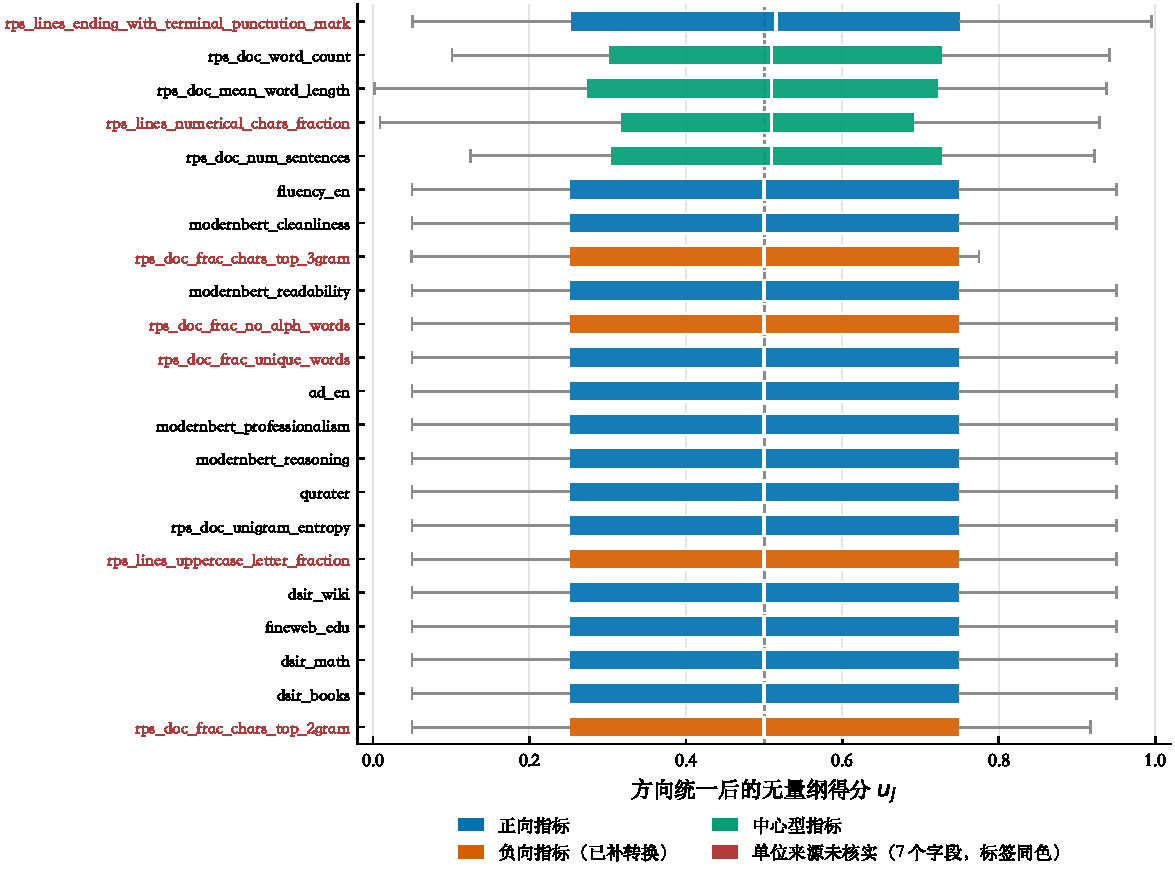
\includegraphics[width=.92\textwidth]{figures/q1-indicator-dist.pdf}
\caption{质量指标分布}
\label{fig:q1-inddist}
\end{figure}

\subsubsection{质量评分模型}\label{sec:q1-score}

质量评分给出两个候选，二者的差别只在样本内的聚合方式。等权候选取 22 个 $u_j$
的算术平均，

\begin{equation}
Q_{\mathrm{eq}}(x)=\frac{1}{J}\sum_{j=1}^{J}u_j(x),\qquad J=22
\end{equation}

稳定性加权候选则以 Huber 位置估计替代算术平均，其权重由指标完整度与排序稳定性
两部分相乘得到：

\begin{equation}
w_j=\frac{r_j}{\sum_{k}r_k},\qquad
r_j=\bigl(c_j\cdot S_j\bigr)^{\alpha}
\end{equation}

式中，$c_j$ 为该指标在 A1 上的完整度（非缺失记录占比），$S_j$ 为域排序稳定性——
将 A1 七个来源域各自的中位数排序重复抽样 1000 次，取该指标秩相关的中位数；
$\alpha$ 为权重指数，主口径取 $\alpha=1$。代入后 18 个指标的权重为 $0.045492$，
其余 4 个因完整度或稳定性略低而略小：\texttt{modernbert\_reasoning} 与
\texttt{modernbert\_professionalism} 的完整度分别为 $0.9997$ 与 $0.9999$，
权重降至 $0.045486$ 与 $0.045490$；\texttt{qurater} 与
\texttt{rps\_lines\_\allowbreak numerical\_chars\_\allowbreak fraction} 的排序稳定性为 $0.9821$，
权重取最小值 $0.0450840$。权重指数取 $\alpha=0.5$ 与取
$\alpha=1$ 在本数据上给出完全相同的样本分，最大绝对差为 0、秩相关为 1，原因在于
各指标的 $r_j$ 本身接近，幂次不足以进一步区分，故不需在 $\alpha$ 上继续搜索。

Huber 位置的阈值取 $\delta=1.345\,s_0$，其中
$s_0=1.4826\,\mathrm{MAD}=0.29484$，得 $\delta=0.39655$。系数 $1.345$ 是标准正态下
$95\%$ 效率对应的常数 \cite{huber_robust_1964}，其含义是残差在 $\delta$ 以内按平方损失处理，超出后转为
线性，从而把单个指标极端取值的影响限制在有界范围。样本分向域级聚合按域内 Huber
位置计算，并给出 $B_Q=2000$ 次记录级 bootstrap 的百分位 $95\%$ 区间 \cite{efron_bootstrap_1979}。权重校准的
过程见图 \ref{fig:q1-weightcal}，完整的评分流程见图 \ref{fig:q1-flowscore}。

两个候选须指定其一作为对外接口，否则问题二与问题三将失去单一的质量输入。本文的
指定依据是可用的判据无法区分二者：全部敏感性场景下两者的样本分高度一致，小样本
人工核查的候选比较亦给出相同的秩相关（见 \ref{sec:q1-sens}）。在此前提下，本文取
稳定性加权 Huber 分 $Q_{\mathrm{huber}}$ 作为操作主分（版本记
\texttt{Q1-q\_huber-v1}），等权分 $Q_{\mathrm{eq}}$ 保留为敏感性对照。该指定的性质
是接口一致性选择，而非统计或人工评审判定的优胜；后文凡称 $Q$ 而未加下标者，均指
$Q_{\mathrm{huber}}$。

\begin{figure}[htp!]
\centering
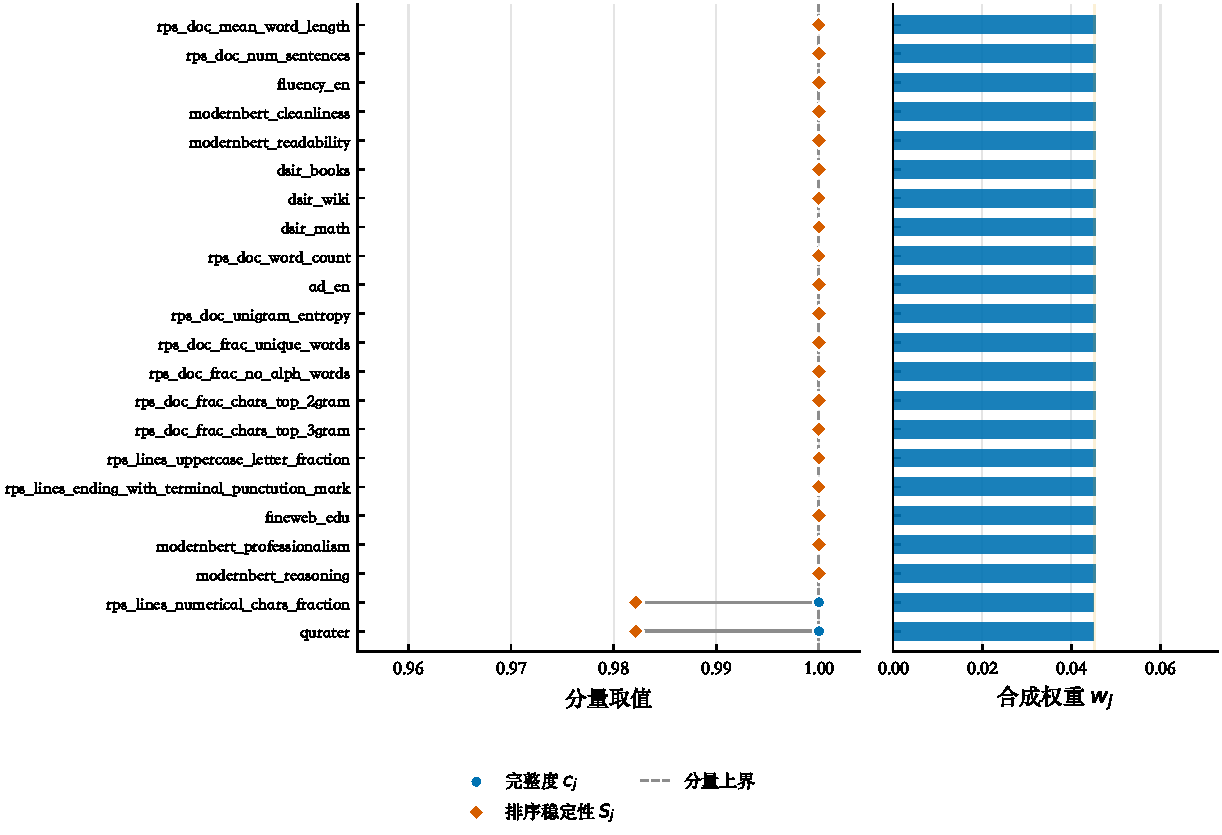
\includegraphics[width=.92\textwidth]{figures/q1-weight-calibration.pdf}
\caption{指标权重的两个构成分量：完整度与排序稳定性}
\label{fig:q1-weightcal}
\end{figure}

\begin{figure}[htp!]
\centering

\includegraphics[width=.92\textwidth]{figures/q1-flow-score.png}
\caption{质量评分的建模流程}
\label{fig:q1-flowscore}
\end{figure}

\subsubsection{冲突度定义与消解规则}\label{sec:q1-conflict}

当不同质量指标对同一文本给出不一致评价时，需要定义冲突、分析成因并给出消解规则。
本文把冲突定义为指标之间的分歧幅度，用行内平均两两绝对分差度量：

\begin{equation}
D(x)=\frac{2}{J(J-1)}\sum_{1\le j<k\le J}\bigl|u_j(x)-u_k(x)\bigr|,
\qquad \binom{22}{2}=231
\end{equation}

式中，$u_j(x)$ 为样本 $x$ 在第 $j$ 个维度上方向统一后的得分。$D$ 只衡量指标之间
是否互相矛盾，不判定哪一项指标有误——在缺少外部真值的条件下，无从判断
\texttt{dsir\_math} 与 \texttt{rps\_doc\_unigram\_\allowbreak entropy} 二者孰是孰非。高冲突
阈值取 A1 各来源域内 $D$ 的第 95 百分位（NumPy \texttt{method=linear} 插值），
A2/A3 一律套用同名域的 A1 阈值以保证跨集可比；消解规则采用稳定性加权 Huber 位置，
并报告两候选之差 $\Delta Q=Q_{\mathrm{huber}}-Q_{\mathrm{eq}}$。

上述阈值属于描述性的上尾判定而非假设检验。$q_{95}$ 是由经验分布定义的分位点，
但有限样本中的实际超阈比例受样本量、离散计数与分位数插值规则影响，并不必然等于
$5\%$；因此本文报告各域实际超阈数与比例，而不把 $5\%$ 当作恒等结果。该阈值用于
描述相对上尾，不代表 $5\%$ 的样本经外部真值确认存在冲突。冲突诊断与消解的完整流程见图
\ref{fig:q1-flowconf}。

\begin{figure}[htp!]
\centering

\includegraphics[width=.92\textwidth]{figures/q1-flow-conflict.png}
\caption{冲突诊断与消解的建模流程}
\label{fig:q1-flowconf}
\end{figure}

\subsubsection{领域配比与损失的定量关系模型}\label{sec:q1-mix}

配比建模只使用 A4/A5 的 512 条训练配方，其配比矩阵
$P\in\mathbb{R}^{512\times17}$ 的每一行满足单纯形约束，待预测的损失矩阵
$Y\in\mathbb{R}^{512\times13}$ 含 13 个目标。配比域比损失目标多 4 个，这 4 个域的
损失无从观测，只能在回归中作为不可观测分量处理，这是模型的结构性限制。配比先做
闭合归一化 $p_{rj}=x_{rj}/\sum_k x_{rk}$，同时保留原始版本用于对照；闭合的必要性
在于行和并非精确为 1，实测范围为 $0.996$--$1.003$。闭合同时改变了零单元的语义，
原始零配比在闭合后仍是零，但非零分量会被等比放大，故 512 条配方的最近邻 $L_1$
距离由 $0$ 变为 $0.0220$。

配比数据在建模前经过一次独立审计，结论如下。A4 至 A15 共 12 个文件、6 组配比—
损失配对，全部通过模式与表头一致性检查，各组行数分别为 $512$、$256$、$256$、
$64$、$63$、$63$，配对表之间的索引顺序完全一致，缺失、重复与多余索引计数均为零；
其中 A6 与 A8 的配比文件同哈希、A12 与 A14 亦同哈希，即这三组检验用的是同一份配比
矩阵，本文在报告检验结果时按此如实并列而不重复计数。512 条训练配方的逐行构成检查
显示：缺失、非法、非有限值与负份额计数全为零，无一行为零和，零份额单元共 $3928$ 个；
原始行和落在 $0.996$ 至 $1.003$ 之间，最大绝对偏差 $0.004$，按
$|{\rm 行和}-1|>0.001$ 计有 $47$ 行超出。这 $47$ 行即闭合归一化在多大程度上有别于
恒等变换的直接证据，也是本文保留原始版本作对照的原因。

主模型为带单纯形约束的多输出收缩回归。记参考域为 $j_0$，模型写成

\begin{equation}
\hat y_{ri}=a_i+\sum_{j\neq j_0}\beta_{ij}\,p_{rj},
\qquad \text{s.t.}\ \sum_{j=1}^{17}\beta_{ij}=0,\quad i=1,\dots,13
\end{equation}

式中，$a_i$ 为第 $i$ 个损失目标的截距，$\beta_{ij}$ 为第 $j$ 个域的配比系数，
约束 $\sum_j\beta_{ij}=0$ 消去"全部域同比例增加"这一不可辨识方向——配比之和恒为
1，系数只有满足该约束才唯一。参考域取 \texttt{uspto\_backgrounds}，其系数固定为 0，
收缩强度由岭参数 $\lambda$ 控制，主口径取 $\lambda=10^{-4}$，由 A4/A5 内部的分组
交叉验证网格选出。

质量评分 $Q$ 是否进入配比模型由参赛队伍自行论证。本文不引入 $Q$，理由是识别性：
若把 $Q$ 作为与配比并列的回归项，模型形如 $p^{\top}b+\theta Q$，而 $Q$ 的域级取值
本身就是各域配比的函数，两者在 $p^{\top}(b+\theta\tilde Q)$ 的意义下不可分别识别，
在缺少外部真值的前提下强行加入只会使系数失去解释。这一判断不停留在论证层面，本文
另做了受限的对照实验加以检验。

检验分两步。第一步查 $Q$ 是否携带配比之外的独立信息：把配比派生的质量特征
$Q_{\mathrm{covered}}(p)$ 加入设计矩阵后，该特征只带来 $1$ 个可辨识秩增量，且审计
确认它在全部 $8$ 个场景中都是 $p$ 的确定性函数，即模型无法把"质量效应"与"配比效应"
分开。第二步看加入后是否真的更准，结果见表 \ref{tab:q1-pq}。该受限比较采用
\texttt{direct\_only} 映射与 \texttt{q\_huber\_candidate} 质量候选；嵌套 OOF 只覆盖
512 条配方中的 478 个共同支持样本。已评估留出集的样本量依次为 1M 的 248、60M 的
248 与 1B 的 64。上述留出集已用于本次比较，故结果是补充性、描述性证据，不是新增盲测，
也不替代主模型的全样本评价。

\begin{table}[htp!]
\centering
\renewcommand\arraystretch{1.2}
\caption{配比派生质量特征对照}\label{tab:q1-pq}
\begin{tabular*}{\textwidth}{@{\extracolsep{\fill}}lccc@{}}
\toprule
评估口径 & 线性 p-only & 二次 p-only & p $+$ 质量特征 \\
\midrule
A4/A5 嵌套 OOF 标准化 RMSE & 0.627628 & 0.595170 & 0.763354 \\
\bottomrule
\end{tabular*}

\vspace{4pt}
\begin{tabular*}{\textwidth}{@{\extracolsep{\fill}}lcc@{}}
\toprule
检验集上相对二次 p-only 的标准化 RMSE 变化 & 切分 & 变化量 \\
\midrule
1M（同尺度） & A6/A7 & $+0.188977$ \\
60M（跨尺度） & A8/A9 & $-0.090549$ \\
1B（跨尺度） & A10/A11 & $+0.045533$ \\
\bottomrule
\end{tabular*}
\end{table}

式中，正值表示加入质量特征后误差增大，三行均以二次 p-only 为基准。结果是
否定的：在 A4/A5 的嵌套交叉验证上，加入质量特征使标准化 RMSE 由 $0.595170$ 升至
$0.763354$，不但没有改善反而明显变差；分尺度看，同尺度的 1M 与跨尺度的 1B 上
同样变差，只有已被接触过的 60M 出现局部改善。这与步骤一的秩增量结论一致——该特征
是配比的重参数化，加入它等于给模型增加一个与配比共线的方向，只会放大方差。

据此本文采用配比单独建模，把 $Q$ 留给问题二的标度律处理。需要强调，这一结论只针对
配比派生的质量特征 $Q_{\mathrm{covered}}(p)$ 这一种构造：它是配比的确定性派生量，
因而本检验不能推广为"质量对损失无影响"，只能说明在当前数据下无法借助它识别出
独立的质量效应。

除主模型外，另设四个对照与敏感性变体，即训练均值空模型（下界）、参考分量 OLS
（截距加 16 个分量、参考系数固定为 0）、Huber 岭回归（$\rho_{1.345}$，用于检验
异常损失的影响）与零友好的二次面（17 个一次项与 136 个两两乘积项，共 153 项）。主模型族在预定的
A4/A5 分组交叉验证中冻结；二次面作为额外的结构敏感性分析报告，不回填主选模。它的
153 个系数由 512 条配方估计，且 511/512 行含零配比，结构零与舍入零未被区分，故需
关注复杂度与零结构带来的稳定性风险；但风险本身不等于已经证明其预测增益为过拟合。
A6--A11 只用于评估冻结后的模型，A12--A15 只用于与估计表比对一致性，不参与调参。配比与各损失目标之间的相关系数
见图 \ref{fig:q1-corr}，本节的建模与验证流程见图 \ref{fig:q1-flowmix}。

\begin{figure}[htp!]
\centering
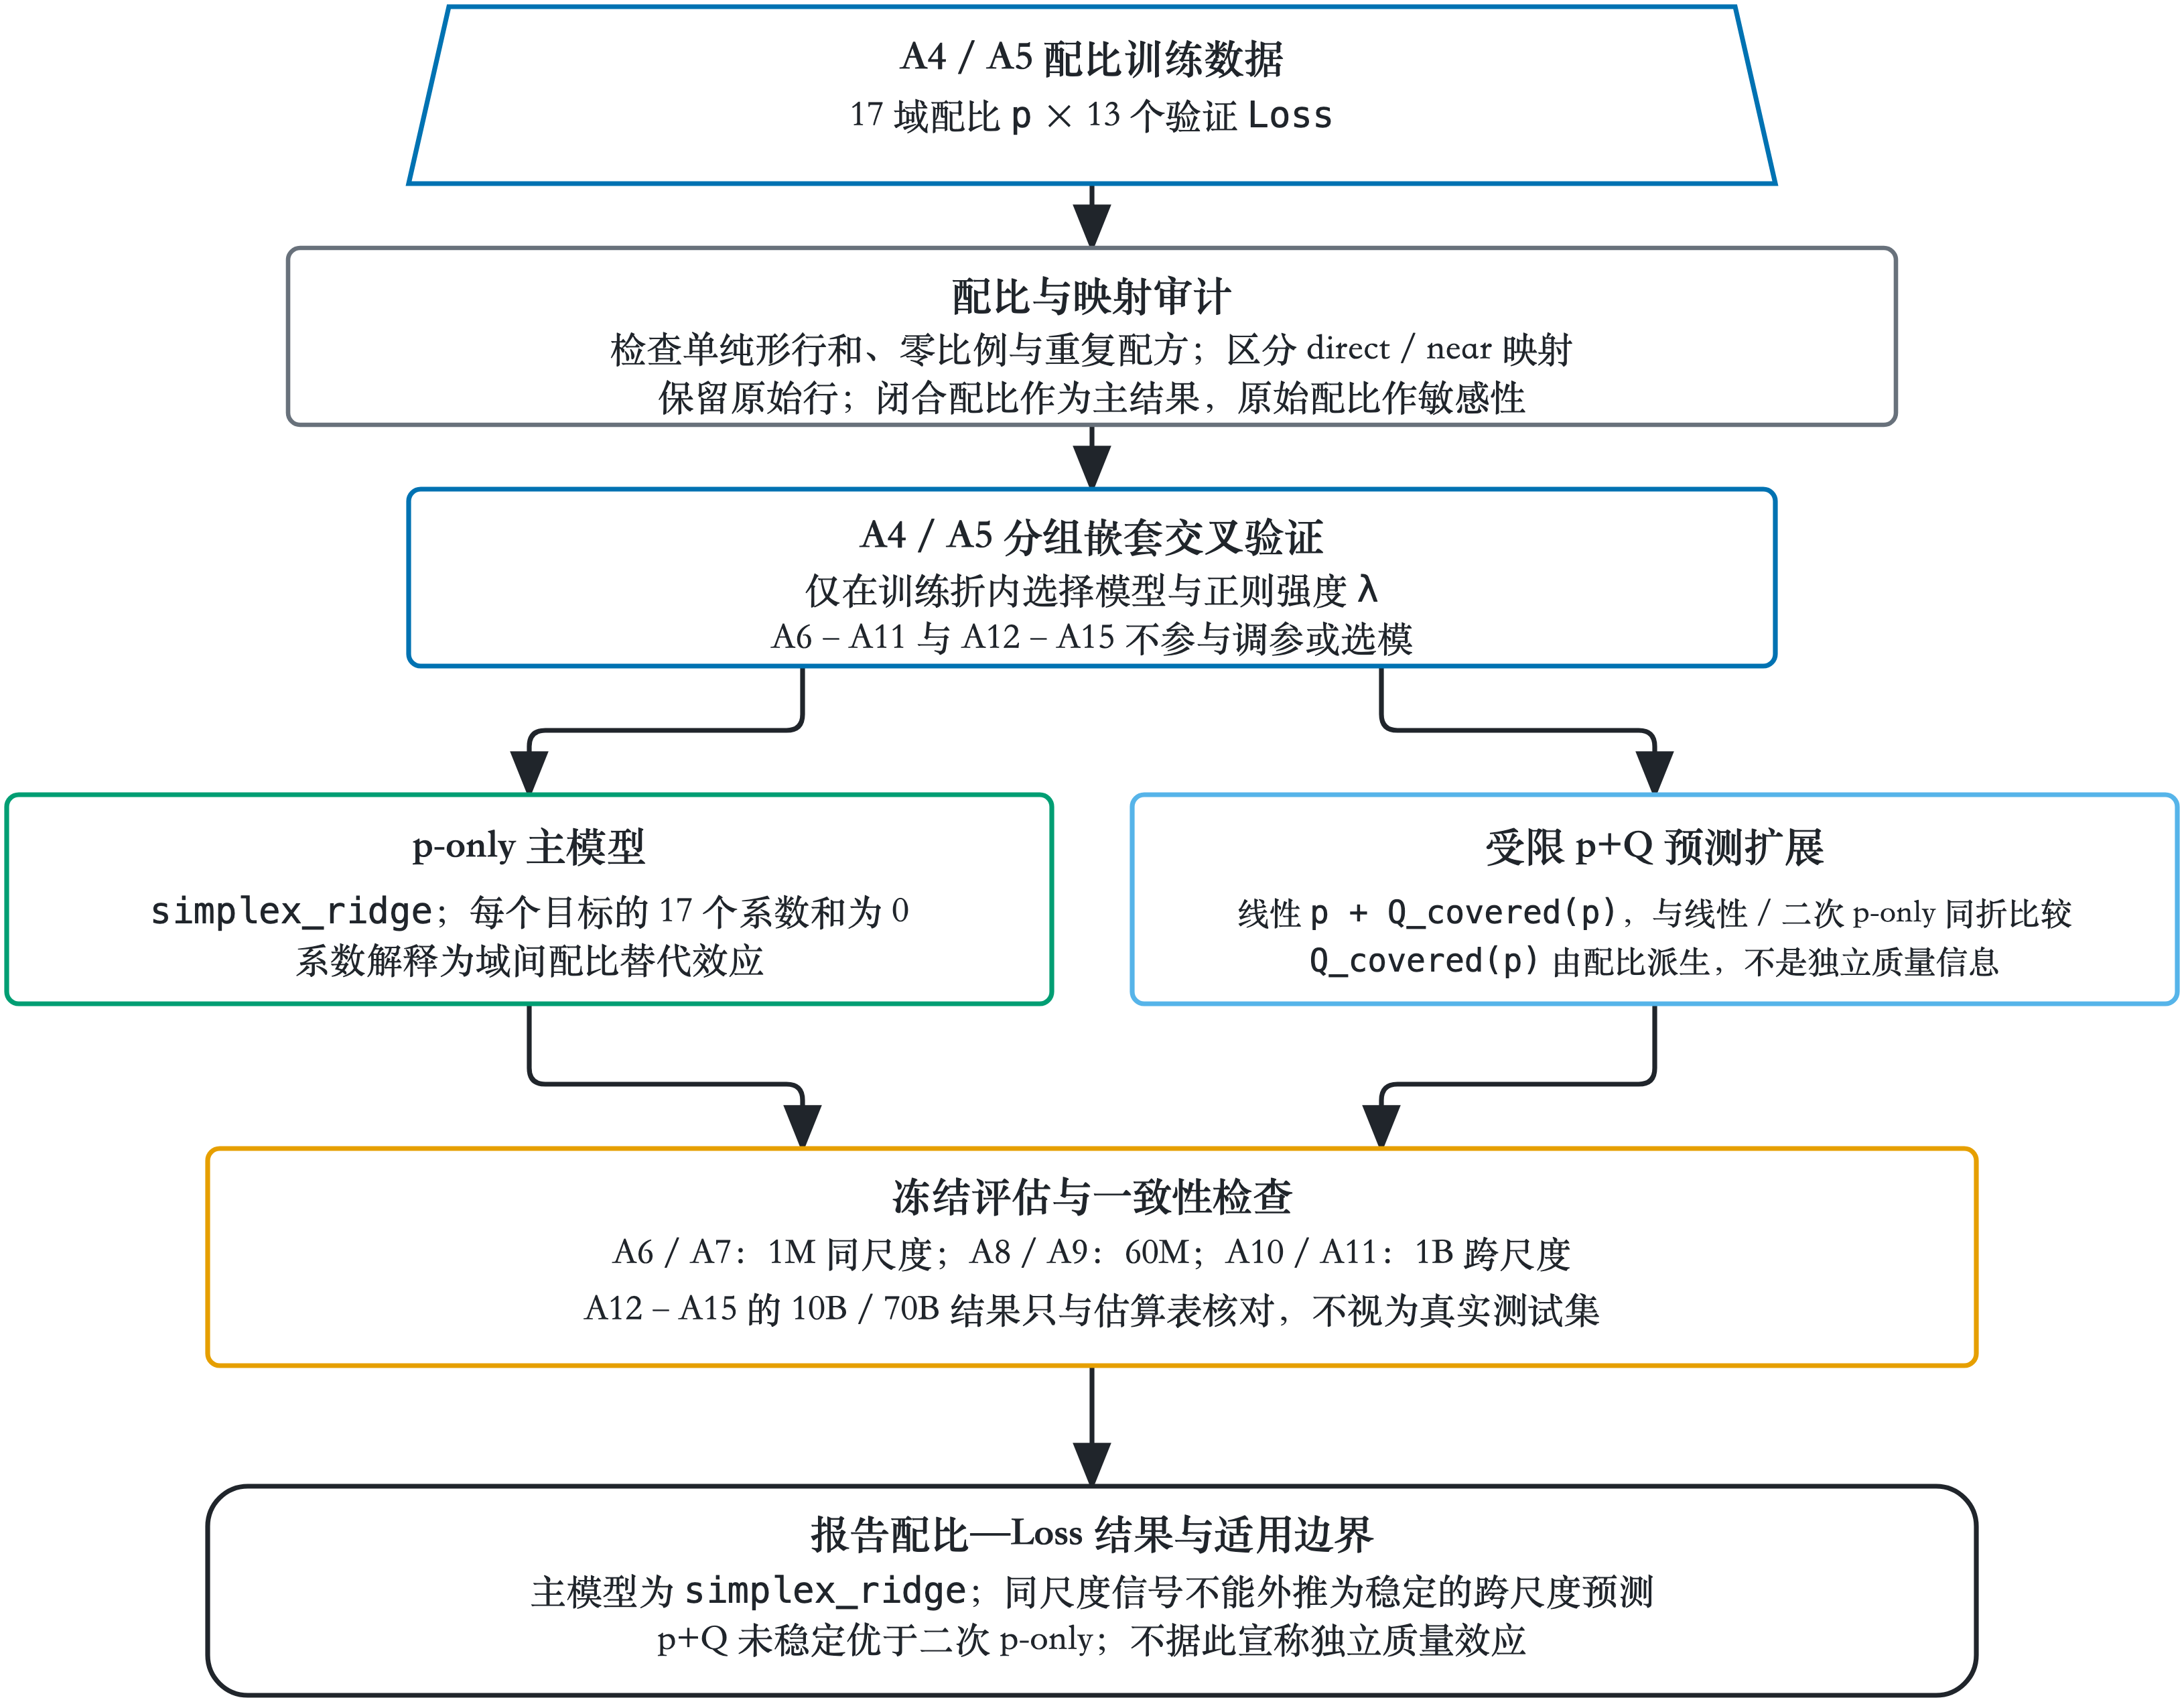
\includegraphics[width=.92\textwidth]{figures/q1-flow-mixture.png}
\caption{配比—损失建模与验证流程}
\label{fig:q1-flowmix}
\end{figure}

\begin{figure}[htp!]
\centering
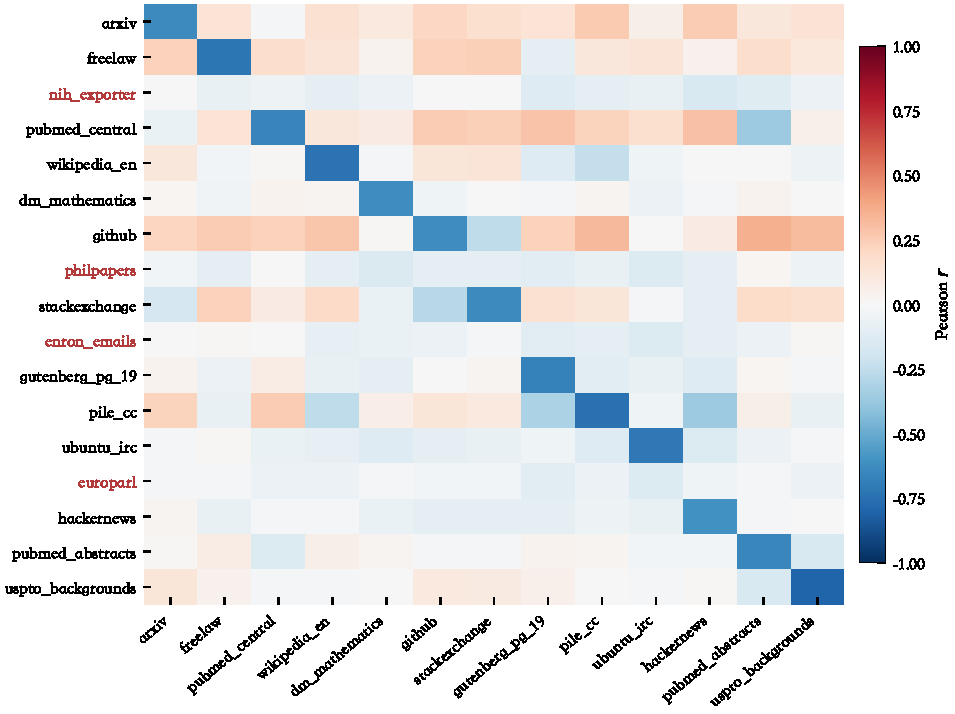
\includegraphics[width=.92\textwidth]{figures/q1-share-loss-corr.pdf}
\caption{配比与损失的相关系数}
\label{fig:q1-corr}
\end{figure}

\subsection{模型求解}

求解流程分四步，依次是归一化校准、权重构造、配比回归与不确定性估计。权重中的域
排序稳定性通过重复抽样估计，Huber 位置用迭代重加权最小二乘求解，配比回归的岭参数
在网格上按分组交叉验证误差选取，替代效应则用配对 bootstrap 给出区间，配比回归部分
的伪代码见表 \ref{alg:q1-solve}。

\begin{table}[htp!]
\centering
\renewcommand\arraystretch{1.2}
\caption{带单纯形约束的多输出回归求解步骤}\label{alg:q1-solve}
\begin{tabularx}{\textwidth}{cX}
\toprule
步骤 & 操作 \\
\midrule
1 & 读入配比矩阵 $P$ 与损失矩阵 $Y$，按行闭合 $p_{rj}\leftarrow x_{rj}/\sum_k x_{rk}$ \\
2 & 按来源分组（\texttt{index}）划分 $K$ 折，保证同组不跨折 \\
3 & \textbf{for} 每个候选 $\lambda$ \textbf{do} 在 $K$ 折上计算标准化 MSE \\
4 & 选 $\hat\lambda=\arg\min_\lambda \mathrm{CV}(\lambda)$，重拟合得 $\hat B,\hat a$ \\
5 & \textbf{if} 用 Huber 变体 \textbf{then} IRLS 迭代至权重收敛（最大 13 轮） \\
6 & 用 $\hat B,\hat a$ 预测 A6--A11，按目标汇总 MAE/RMSE/$R^2$/Spearman \\
7 & 对每个域对做 500 次配对 bootstrap，得 10 个百分点替代效应的 95\% 区间 \\
\bottomrule
\end{tabularx}
\end{table}

求解的可靠性可由三项收敛证据支持：Huber 变体在 13 个损失目标上全部收敛，最大迭代
13 轮；各目标被降权的训练配方数最多为 24 条（\texttt{arxiv} 与 \texttt{github}），
权重低于 $0.5$ 的仅 1 条；参考分量 OLS 的设计矩阵条件数在五折内为
$[198.7,209.4,235.0,204.9,206.6]$，远低于 $10^7$ 的病态告警阈值。

\subsection{结果分析}

\subsubsection{质量评分结果}\label{sec:q1-scoreres}

A1 七域的域级质量评分见表 \ref{tab:q1-domain}，两候选的宏平均分别为 $0.49622$
（等权，$95\%$ 区间 $[0.49491,0.49763]$）与 $0.49848$（Huber，
$[0.49657,0.50043]$）。两候选给出的排名基本一致，分歧集中在 \texttt{book} 与
\texttt{github} 两个域：等权分把 \texttt{book} 排在 \texttt{github} 之前
（$0.43160$ 对 $0.40450$），Huber 分则把两者拉近（$0.42875$ 对 $0.38948$），
差异的来源可从 \ref{sec:q1-sens} 的冲突分析中找到——\texttt{book} 正是指标分歧
最大的域。各域评分及其区间见图 \ref{fig:q1-domscores}。两候选的取舍依据来自小样本
人工核查与全部敏感性场景，其证据与边界在 \ref{sec:q1-sens} 中一并报告。

\begin{table}[htp!]
\centering
\renewcommand\arraystretch{1.2}
\caption{各来源域的域级质量评分（等权与加权两候选）}\label{tab:q1-domain}
\begin{tabular*}{\textwidth}{@{\extracolsep{\fill}}llccc@{}}
\toprule
数据集 & 来源域 & 记录数 & $Q_{\mathrm{eq}}$ & $Q_{\mathrm{huber}}$ \\
\midrule
A1 & arxiv         & 1419   & 0.53210 & 0.56133 \\
A1 & book          & 171      & 0.43160 & 0.42875 \\
A1 & c4            & 10000  & 0.57053 & 0.57673 \\
A1 & commoncrawl   & 9640   & 0.53401 & 0.53597 \\
A1 & github        & 10000  & 0.40450 & 0.38948 \\
A1 & stackexchange & 10000  & 0.51734 & 0.51837 \\
A1 & wikipedia     & 10000  & 0.48349 & 0.47871 \\
\midrule
A2 & arxiv         & 17523  & 0.53096 & 0.55997 \\
A3 & github        & 203752 & 0.40394 & 0.38887 \\
\bottomrule
\end{tabular*}
\end{table}

\begin{figure}[htp!]
\centering
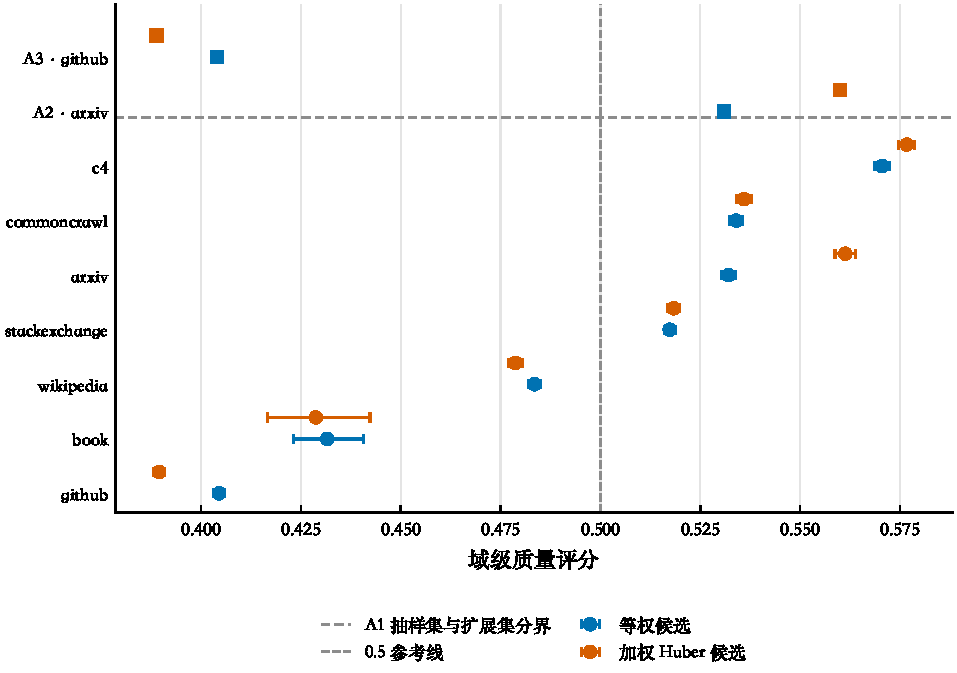
\includegraphics[width=.92\textwidth]{figures/q1-domain-scores.pdf}
\caption{各来源域的域级质量评分及估计区间}
\label{fig:q1-domscores}
\end{figure}

同域迁移检验的结果见表 \ref{tab:q1-transfer}。A2 与 A3 分别是 A1 中 arxiv 与
github 两个域的扩展集，由于归一化参数只在 A1 上拟合，同域扩展集相对抽样集的评分偏移
即反映标量层面的可比性。四个差值的 $95\%$ 区间全部跨零，点估计均在千分位以下，
说明在 A1 上拟合的参数直接套用到两个扩展集时，域级评分没有可检出的偏移。差值及其
区间另见图 \ref{fig:q1-transfer}。这一比较限定在标量层面，其范围由数据的可得性决定：
A2 与 A3 的特征文件不含原文内容字段（两集的 \texttt{content} 字段命中记录数均为 0），
因此本节的迁移检验只能做到标量层面。原文层面的核验在 A1 上已经完成——见
\ref{sec:q1-sens} 的逐记录 Unicode 完整性审计与小样本双评者核查；A2/A3 的原文
层面核验则不在本文可及范围内，需在取得原文后才能进行。

\begin{table}[htp!]
\centering
\renewcommand\arraystretch{1.2}
\caption{同域扩展集相对抽样集的评分偏移（bootstrap 区间）}\label{tab:q1-transfer}
\begin{tabular*}{\textwidth}{@{\extracolsep{\fill}}llcc@{}}
\toprule
对比 & 候选 & 差值 & $95\%$ 区间 \\
\midrule
A2 arxiv $-$ A1 arxiv   & $Q_{\mathrm{eq}}$    & $-0.00114$ & $[-0.00288,\ 0.00070]$ \\
A2 arxiv $-$ A1 arxiv   & $Q_{\mathrm{huber}}$ & $-0.00136$ & $[-0.00399,\ 0.00128]$ \\
A3 github $-$ A1 github & $Q_{\mathrm{eq}}$    & $-0.00056$ & $[-0.00185,\ 0.00086]$ \\
A3 github $-$ A1 github & $Q_{\mathrm{huber}}$ & $-0.00061$ & $[-0.00211,\ 0.00085]$ \\
\bottomrule
\end{tabular*}
\end{table}

\begin{figure}[htp!]
\centering
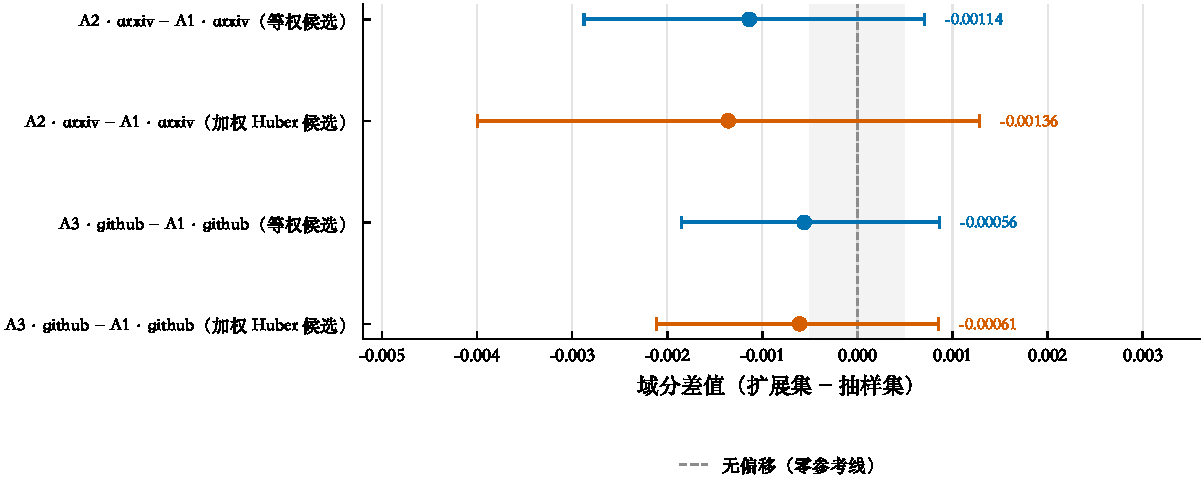
\includegraphics[width=.92\textwidth]{figures/q1-domain-transfer.pdf}
\caption{同域扩展集与 A1 的域分差值}
\label{fig:q1-transfer}
\end{figure}

\subsubsection{冲突分析与消解结果}\label{sec:q1-confres}

各域的中位冲突度与 $q_{95}$ 阈值见表 \ref{tab:q1-conflict}。\texttt{arxiv} 的中位
冲突度最高（$0.4382$），\texttt{stack\-exchange} 最低（$0.2712$），两者相差
$0.167$；
扩展集的冲突度与同域 A1 高度接近，A2 为 $0.4393$、A3 为 $0.3236$。高冲突率方面，
按各域自身的经验第 95 百分位设定阈值后，样本充足的五个域超阈比例恰为 $5.00\%$，
\texttt{arxiv} 为 $5.00\%$（71/1419），\texttt{book} 为 $5.26\%$（9/171）。后者的
来自有限样本的整数计数：\texttt{book} 域 171 条记录中有 9 条超阈，即 $9/171=5.26\%$。
结果文件中的 \texttt{threshold\_tie\_rate} 为 $0$，故没有证据把偏离归因于阈值处并列；
它体现的是有限样本下经验分位点对应的实际计数不必恰为 $0.05n$。A2 的 $0.0447$ 与
A3 的 $0.0514$ 则说明扩展集在套用 A1 阈值后，落入高冲突区的比例与原集基本一致。
各域的冲突度分布与阈值见图 \ref{fig:q1-confdist}。

\begin{table}[htp!]
\centering
\renewcommand\arraystretch{1.2}
\caption{各来源域的冲突度水平与高冲突判定阈值}\label{tab:q1-conflict}
\begin{tabular*}{\textwidth}{@{\extracolsep{\fill}}llccc@{}}
\toprule
数据集 & 来源域 & 中位冲突度 & $q_{95}$ 阈值 & 高冲突率 \\
\midrule
A1 & arxiv         & 0.4382 & 0.4660 & 0.0500 \\
A1 & book          & 0.4098 & 0.4476 & 0.0526 \\
A1 & c4            & 0.3241 & 0.4188 & 0.0500 \\
A1 & commoncrawl   & 0.2883 & 0.3834 & 0.0500 \\
A1 & github        & 0.3232 & 0.4294 & 0.0500 \\
A1 & stackexchange & 0.2712 & 0.3598 & 0.0500 \\
A1 & wikipedia     & 0.3069 & 0.4079 & 0.0500 \\
\midrule
A2 & arxiv         & 0.4393 & 0.4660 & 0.0447 \\
A3 & github        & 0.3236 & 0.4294 & 0.0514 \\
\bottomrule
\end{tabular*}
\end{table}

\begin{figure}[htp!]
\centering
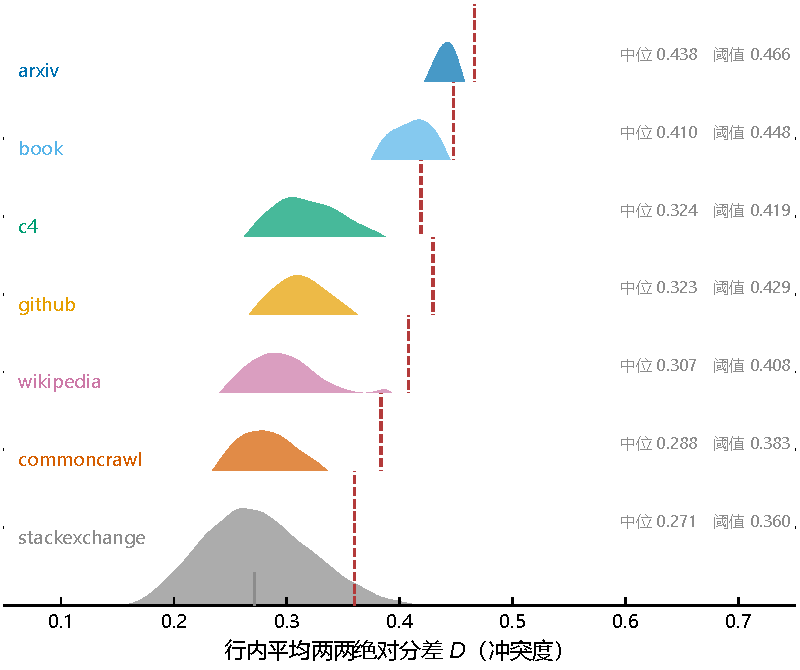
\includegraphics[width=.92\textwidth]{figures/q1-conflict-dist.pdf}
\caption{域内冲突度分布}
\label{fig:q1-confdist}
\end{figure}

指标对层面的分歧结构更为具体。A1 七域宏平均下冲突最激烈的三对依次是
\texttt{dsir\_math} 与 \texttt{rps\_doc\_unigram\_\allowbreak entropy}（$0.5993$）、
\texttt{dsir\_wiki} 与同一元熵指标（$0.5963$）、\texttt{dsir\_books} 与同一元熵
指标（$0.5953$），三对均含 \texttt{rps\_doc\_unigram\_\allowbreak entropy}，其成因可以解释：
dsir 系列衡量文本与某一参考语料的相似度，而一元熵衡量文本自身词汇分布的分散度，
后者高的文本未必与任何参考语料接近，两者的评价对象并不相同。231 个指标对的分歧
结构见图 \ref{fig:q1-pairconf}。

\begin{figure}[htp!]
\centering
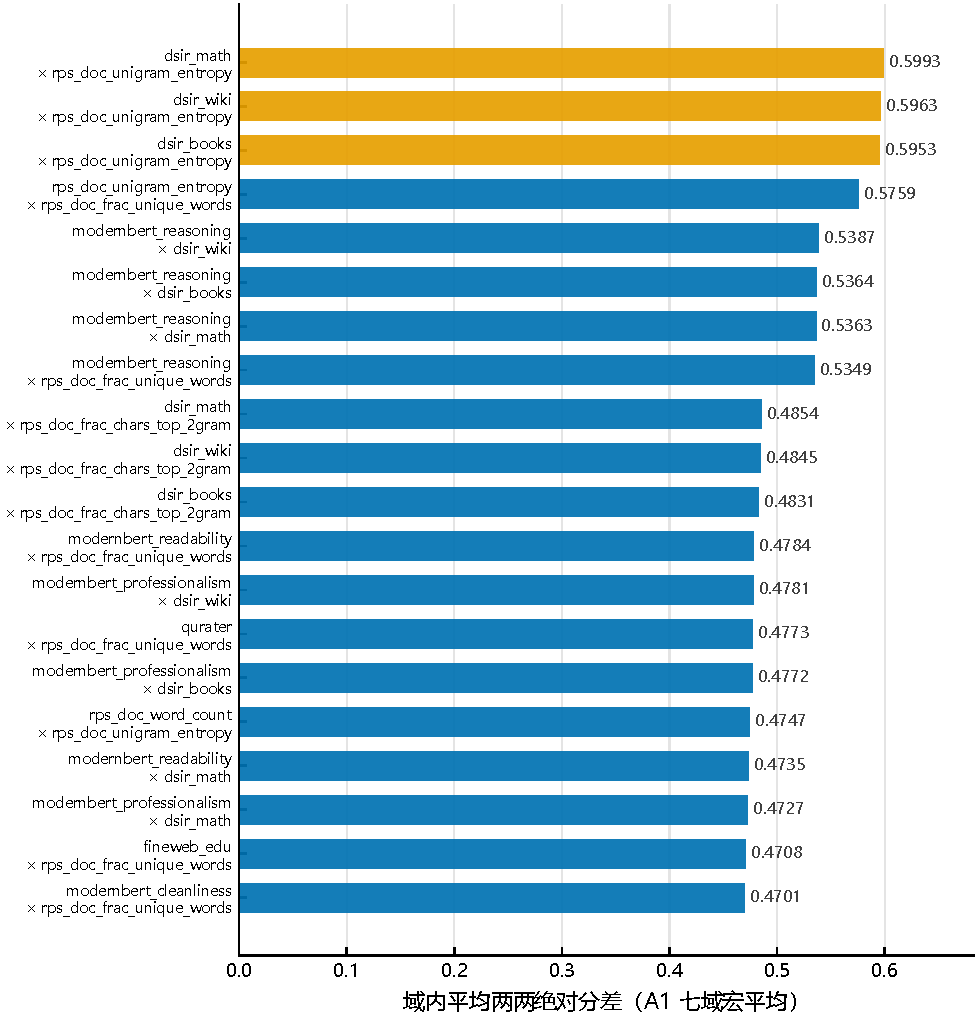
\includegraphics[width=.92\textwidth]{figures/q1-pair-conflict.pdf}
\caption{指标两两冲突度分布}
\label{fig:q1-pairconf}
\end{figure}

消解后的评分为 $Q_{\mathrm{huber}}$。在高冲突组内，两候选的差值方向并不统一，
\texttt{github}（$-0.0497$）、\texttt{wikipedia}（$-0.0330$）与 \texttt{c4}
（$-0.0056$）为负，而 \texttt{arxiv}（$+0.0438$）、\texttt{book}（$+0.0393$）与
\texttt{commoncrawl}（$+0.0127$）为正。\texttt{book} 域的分歧幅度尤为突出，其高
冲突组的 $|\Delta Q|$ 中位数为 $0.0393$，是其余组 $0.01973$ 的两倍，与表
\ref{tab:q1-conflict} 中 \texttt{book} 唯一非 $0.05$ 的高冲突率互为印证。

扩展集上的复核分两个层次。标量层面，A2 与 A3 相对 A1 的域内中位冲突度之差与高
冲突率之差共四个区间全部跨零，点估计均在千分位以下，即没有可检出的系统性偏移。
排序层面更能说明"主要结论在扩展集同样成立"：A2 与 A1 之间 231 个指标对的分歧排序
Spearman 相关为 $0.99963$，A3 与 A1 之间为 $0.99949$，A1 上分歧最大的前十对指标
在 A2 上命中九对、在 A3 上十对全中。也就是说，扩展集不仅没有推翻抽样集上的冲突
结论，连指标对之间的相对分歧次序都几乎原样保持。两个层次的复核结果分别见表
\ref{tab:q1-conflict} 与图 \ref{fig:q1-confext}。

\begin{figure}[htp!]
\centering
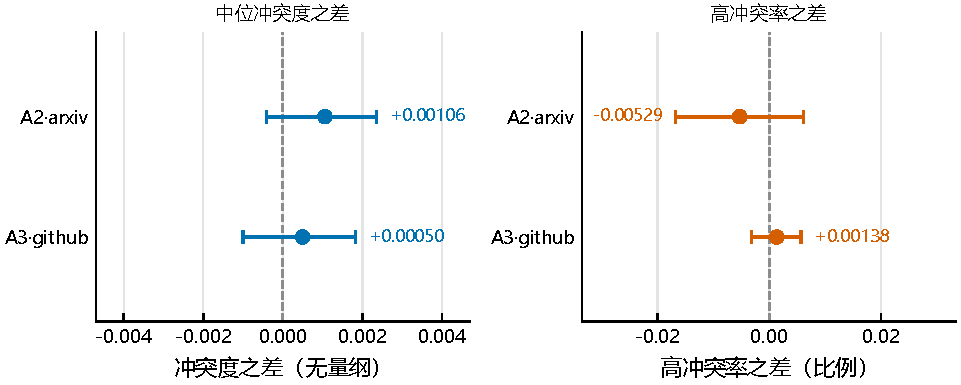
\includegraphics[width=.92\textwidth]{figures/q1-conflict-external.pdf}
\caption{扩展集冲突指标复核}
\label{fig:q1-confext}
\end{figure}
冲突度与评分分歧幅度的关系见图 \ref{fig:q1-conflict-effect}。

\begin{figure}[htp!]
\centering
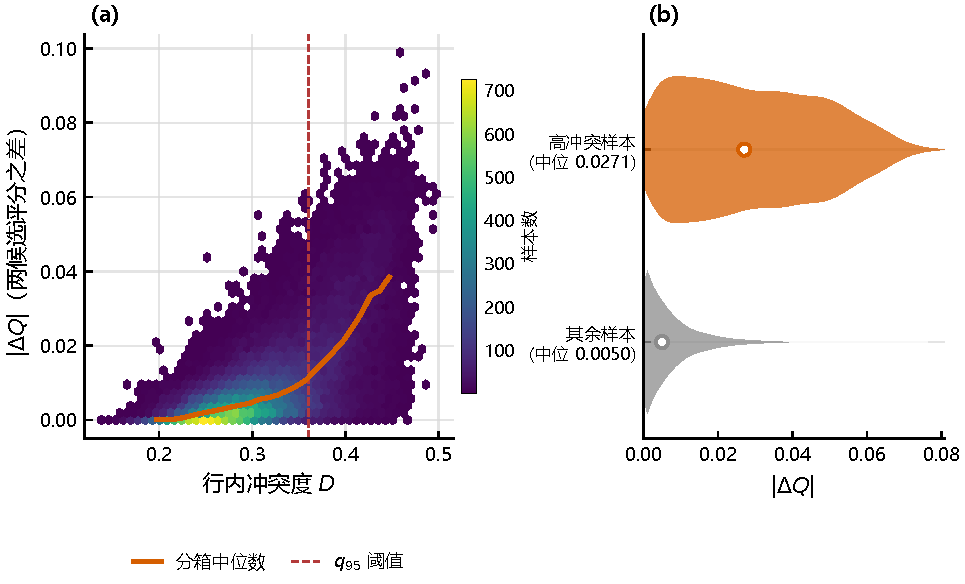
\includegraphics[width=.92\textwidth]{figures/q1-conflict-effect.pdf}
\caption{冲突度与评分分歧幅度的关系}
\label{fig:q1-conflict-effect}
\end{figure}


\subsubsection{配比—损失模型结果}\label{sec:q1-mixres}

模型选择的结果见表 \ref{tab:q1-select}。三个主要候选的差别不大但有稳定顺序，单纯形
岭回归的分组交叉验证标准化 MSE 为 $0.39860$，略优于参考分量 OLS 的 $0.40032$，
两者都远优于训练均值空模型的 $1.00448$。模型族的交叉验证对比见图
\ref{fig:q1-sel}。
主模型相对基线的逐目标改善见图 \ref{fig:q1-model-gain}。
\begin{figure}[htp!]
\centering
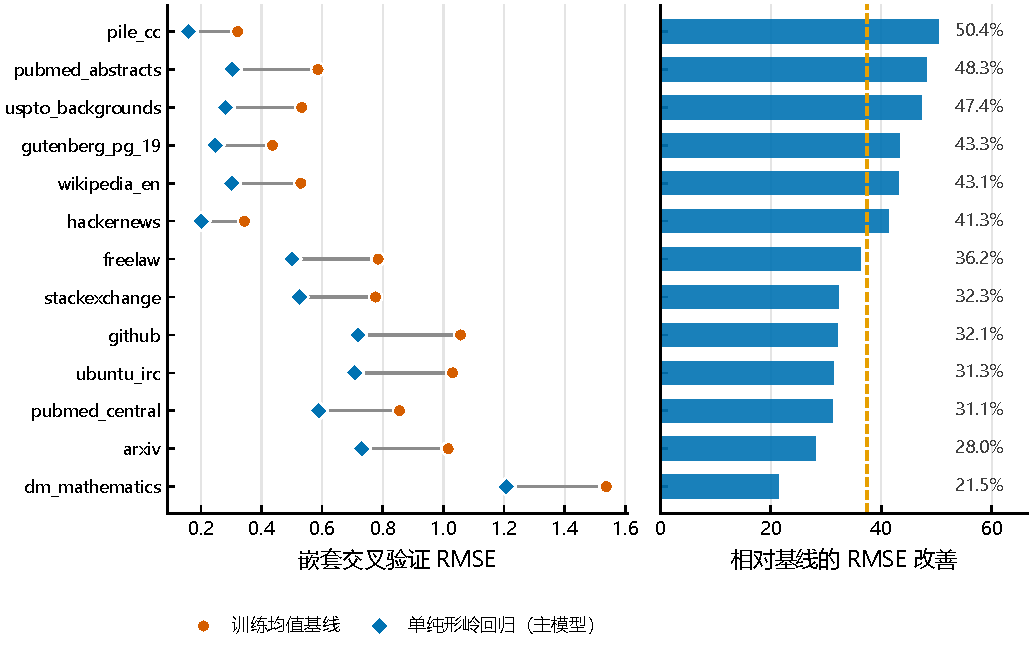
\includegraphics[width=.92\textwidth]{figures/q1-model-gain.pdf}
\caption{主模型相对训练均值基线的拟合误差改善}
\label{fig:q1-model-gain}
\end{figure}


\begin{table}[htp!]
\centering
\renewcommand\arraystretch{1.2}
\caption{三种配比模型族的分组交叉验证误差}\label{tab:q1-select}
\begin{tabular*}{\textwidth}{@{\extracolsep{\fill}}lccc@{}}
\toprule
模型 & 标准化 MSE$\downarrow$ & 正则强度 $\lambda$ & 角色 \\
\midrule
单纯形岭回归（主模型） & 0.39860 & $10^{-4}$ & 选中 \\
参考分量 OLS           & 0.40032 & --- & 对照 \\
Huber 岭回归           & 0.40165 & $3.16\times10^{-5}$ & 稳健性敏感性 \\
二次面（153 项）       & 0.34238 & $0.2848$ & 非线性敏感性 \\
训练均值空模型         & 1.00448 & --- & 下界 \\
\bottomrule
\end{tabular*}
\end{table}

\begin{figure}[htp!]
\centering
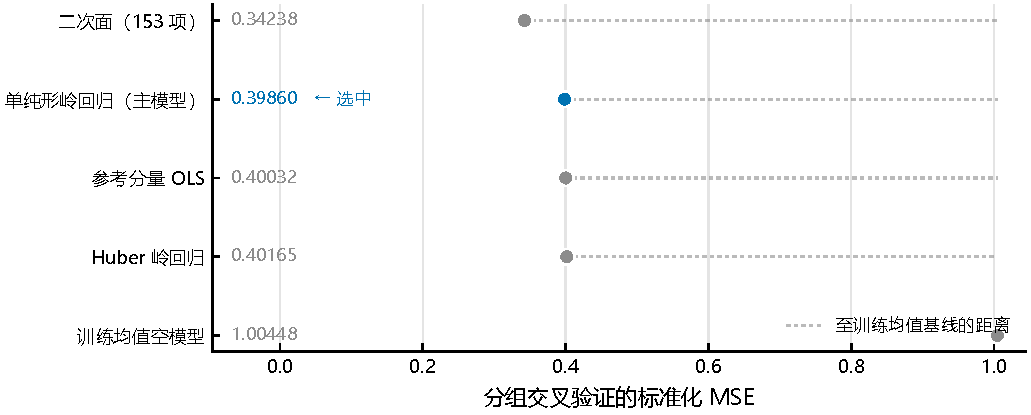
\includegraphics[width=.92\textwidth]{figures/q1-model-selection.pdf}
\caption{三种配比模型族的分组交叉验证误差}
\label{fig:q1-sel}
\end{figure}

主模型在 A4/A5 上的嵌套交叉验证给出宏平均 $R^2=0.59923$、Spearman $\rho=0.82077$、
MAE $=0.41972$、RMSE $=0.49780$，五折的外层选模全部选中同一个模型族，选模流程本身
稳定。冻结检验集与估计表上的表现见表 \ref{tab:q1-holdout}。

\begin{table}[htp!]
\centering
\renewcommand\arraystretch{1.2}
\caption{各检验尺度上的预测误差与秩相关（13 个目标宏平均）}\label{tab:q1-holdout}
\begin{tabular*}{\textwidth}{@{\extracolsep{\fill}}llcccc@{}}
\toprule
数据 & 尺度关系 & MAE$\downarrow$ & RMSE$\downarrow$ & $R^2\uparrow$ & Spearman$\uparrow$ \\
\midrule
A6/A7（1M）    & 同尺度     & 0.3876 & 0.4539 & $\mathbf{+0.6189}$ & 0.8327 \\
A8/A9（60M）   & 跨尺度     & 1.5125 & 1.5590 & $-7.9336$ & 0.8314 \\
A10/A11（1B）  & 跨尺度     & 3.1830 & 3.1970 & $-810.12$ & 0.7268 \\
A12/A13（10B） & 外推估计表 & 3.5730 & 3.6016 & $-236.86$ & 0.4896 \\
A14/A15（70B） & 外推估计表 & 3.9556 & 3.9848 & $-385.31$ & 0.4132 \\
\bottomrule
\end{tabular*}
\end{table}

同尺度的 A6/A7 上模型表现可用，$R^2$ 为 $+0.619$；跨到 60M 与 1B 后 $R^2$ 急剧
转负，但同期 Spearman 仍保持在 $0.73$--$0.83$。二者的差异指向不同的失效机制：
$R^2$ 的负值来自尺度失配——随训练尺度增大，各域验证损失的整体水平下降，而主模型
的系数在 1M 尺度上估计、不含任何尺度项，无法跟随均值漂移；Spearman 则说明模型的
排序能力仍然保留。据此，该模型的适用范围限定为同一训练尺度内的配比筛选，不能作为
跨尺度的定量外推工具。同尺度留出集上的观测值与预测值对照见图 \ref{fig:q1-holdout}，
跨尺度 RMSE 见图 \ref{fig:q1-crossscale}。

\begin{figure}[htp!]
\centering

\includegraphics[width=.9\textwidth]{figures/q1-holdout-1m.pdf}
\caption{同尺度留出集上预测损失与观测损失的一致性}
\label{fig:q1-holdout}
\end{figure}

\begin{figure}[htp!]
\centering
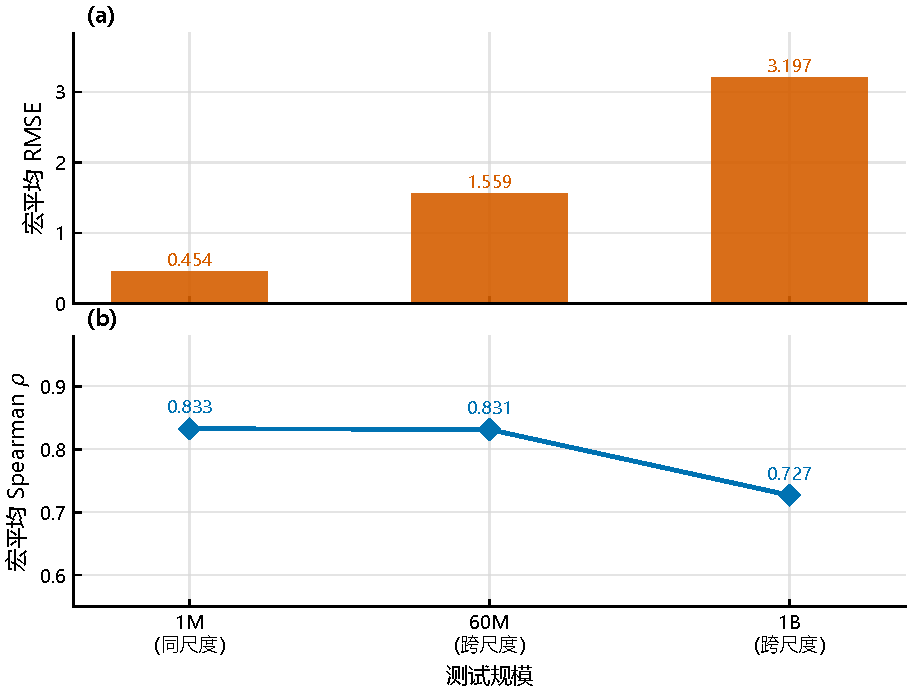
\includegraphics[width=.92\textwidth]{figures/q1-cross-scale.pdf}
\caption{跨尺度检验表现}
\label{fig:q1-crossscale}
\end{figure}

替代效应的方向结构见表 \ref{tab:q1-subst}。136 个域对中有 106 对在训练集上有足够
份额支持 10 个百分点的替代，其 1378 个目标与域对组合的区间中，214 个全为正、
535 个全为负、629 个跨零。区间跨零占近一半，说明多数替代方向在本数据上尚无定论。
这些区间条件于已选模型族、已选 $\lambda$ 与观测训练分布，逐点计算且未做多重比较
校正，系数只反映关联而非因果效应，故区间本身不作为显著性结论。替代关联系数见图
\ref{fig:q1-subst}。

\begin{table}[htp!]
\centering
\renewcommand\arraystretch{1.2}
\caption{配比替代效应区间估计的方向构成}\label{tab:q1-subst}
\begin{tabular*}{\textwidth}{@{\extracolsep{\fill}}lcc@{}}
\toprule
类别 & 数量 & 占比 \\
\midrule
受支持的域对 & 106 & 77.9\%（占 136 对） \\
\quad 区间全为正 & 214 & 15.5\% \\
\quad 区间全为负 & 535 & 38.8\% \\
\quad 区间跨零   & 629 & 45.7\% \\
不受支持的域对 & 30 & 22.1\%（占 136 对） \\
\bottomrule
\end{tabular*}
\end{table}

\begin{figure}[htp!]
\centering
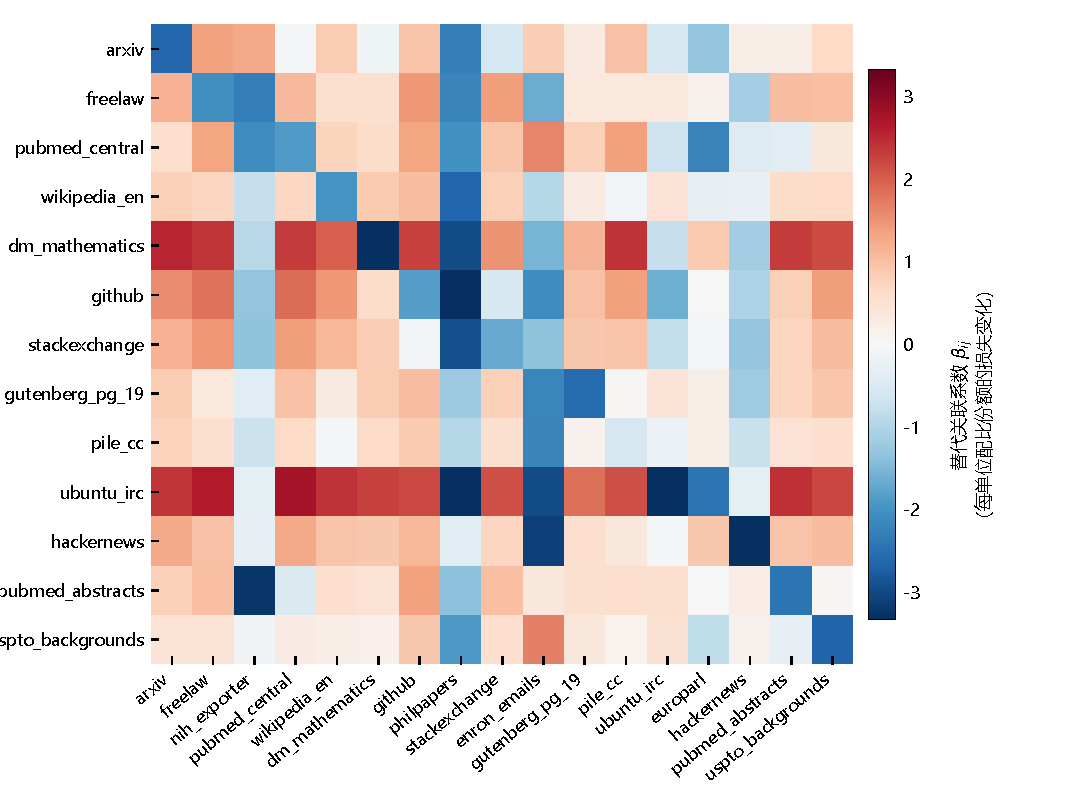
\includegraphics[width=.92\textwidth]{figures/q1-substitution.pdf}
\caption{配比替代效应系数结构}
\label{fig:q1-subst}
\end{figure}
1768 个目标—域组合中有 895 个替代方向稳定；该统计是配对区间方向判定，并不表示
每个方向都具有显著的实际效应。各组合的方向确定性见图 \ref{fig:q1-substitution-volcano}。

\begin{figure}[htp!]
\centering
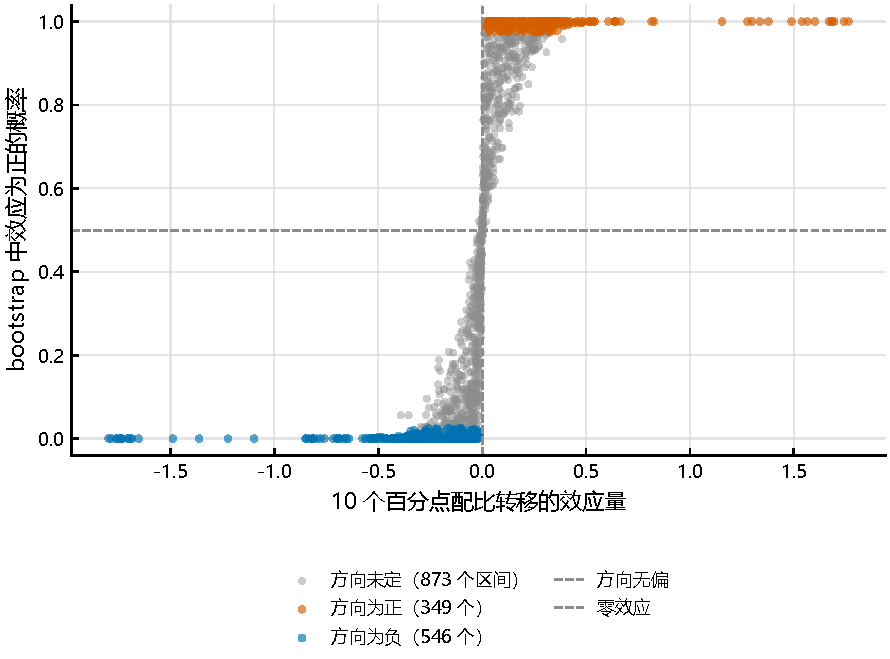
\includegraphics[width=.92\textwidth]{figures/q1-substitution-volcano.pdf}
\caption{替代方向确定性}
\label{fig:q1-substitution-volcano}
\end{figure}


各检验集上误差最大的目标一并列出：A6/A7 上为
\texttt{the\_pile\_dm\_mathematics\_\allowbreak val\_loss}（RMSE $1.1634$），A8/A9 与 A10/A11
上均为 \texttt{github}（$2.6333$ 与 $4.4280$），A12/A13 与 A14/A15 上均为
\texttt{ubuntu\_irc}（$4.4513$ 与 $4.9323$）。最大的预测五分位偏差出现在
\texttt{dm\_mathematics} 的第 5 组，预测减观测为 $-0.5174$，即高损失区存在系统性
低估。

\subsection{模型验证与灵敏度分析}\label{sec:q1-sens}

本节的验证围绕一个目标：考察前述结论对预处理参数、权重构造与数据中异常记录的
稳定性，主要场景见表 \ref{tab:q1-sens}。

\begin{table}[htp!]
\centering
\renewcommand\arraystretch{1.2}
\caption{评分对字段与权重设定的敏感性}\label{tab:q1-sens}
\begin{tabular*}{\textwidth}{@{\extracolsep{\fill}}lccc@{}}
\toprule
敏感性场景 & 样本分 P95 绝对差$\downarrow$ & 排序 Spearman$\uparrow$ & 判读 \\
\midrule
剔除上游公式未追溯字段 & 0.113048 & 0.872404 & 影响最大，排序仍稳 \\
Huber 阈值 $\delta\times0.5$ & --- & 0.980320 & 影响有限 \\
权重指数 $\alpha=0.5$ & $0$ & $1.000000$ & 完全等价 \\
剔除带单位标记的 A1 行 & $10^{-6}$ & $1.000000$ & 可忽略 \\
\bottomrule
\end{tabular*}
\end{table}

影响最剧烈的是剔除 7 个上游公式未追溯字段，A1 样本分的 P95 绝对差达 $0.113048$、
最大差 $0.255681$，A2 上的秩相关降到 $0.729556$。这一场景的作用是给出语义不确定
性的上界探测：把 7 个字段整体移出后评分变化的上限即在上述量级，它衡量的是评分对
这批语义未定字段的依赖程度，而不是数据存在错误的证据——独立复算已表明其取值尺度
为百分数存储，超过 100 的少数记录源自重叠 $n$-gram 的重复计数。基于这一量级，本文
不把 $Q$ 称为 22 路信号的完整综合，而称其为受限候选分，并在正文中逐一列明仍然存疑
的字段。相比之下，Huber 阈值折半只带来 $0.007374$ 的宏平均位移（秩相关 $0.980$），
权重指数 $\alpha$ 的选择则完全不影响结果。

参数与字段层面的稳健性之外，评分还须经过一次独立于建模过程的外部核验。受人工评审
工作量限制，本研究未实施 793 条样本的双人全量评分，而采用 30 条小样本双评者核查，
其中 24 条代表性样本用于候选比较，6 条诊断性样本用于案例检查。抽样范围须交代清楚：
30 条并非从全部 793 条中随机抽取，而是取自其中长度不超过 8000 字符的 526 条
合格记录，因此只覆盖 7 个来源域中的 6 个，\texttt{book} 域因无一条合格记录而
完全缺席；候选的百分位排名仍在全部 793 条上计算。这一限制意味着下述一致性结论
不适用于长文本，也不适用于 \texttt{book} 域。两位评审的总体质量
评分具有一定一致性，二次加权 Cohen $\kappa=0.765$，评审间 Spearman 相关为
$0.806$。但两份回收表顺序相同，评审材料采用中文机译辅助版本，独立评分过程亦未得到
记录核实。因此该核查仅作为有限的评分一致性与候选比较证据，不构成全量人工效度验证，
也不构成对英文原文的直接验证。A2/A3 的原文链接仅覆盖部分记录——A2 为
$1419/17523$、A3 为 $10000/203752$，未链接的 $16104$ 与 $193752$ 条不纳入
原文层面的核验。在 24 条代表性样本上，$Q_{\mathrm{eq}}$ 与 $Q_{\mathrm{huber}}$ 对
人工共识评分的 Spearman 相关均为 $0.5667$，两者相关差的配对 bootstrap $95\%$ 区间
为 $[-0.0590,0.0623]$，跨零。据此，本文按接口一致性选择 $Q_{\mathrm{huber}}$ 作为
主 $Q$，并以 $Q_{\mathrm{eq}}$ 进行敏感性分析，不将该选择表述为人工或统计验证的
胜出。

污染敏感性另作一项检验。对 A1 的原文做逐记录的 Unicode 完整性审计，按窄口径
（格式字符与除制表、换行外的控制字符）检出 428 条，按宽口径（并含私用区与非法
码点）检出 463 条，分别占 51230 条的 $0.836\%$ 与 $0.904\%$。题目材料的历史
报告中曾出现 334 条这一计数，但现有扫描规则无法复现，故不作为本次结果引用。两套
规则各自对应一组敏感性结果，将相应记录分别从阈值、权重、Huber 阈值与指标对排序的
估计中剔除后：权重向量的 $L_1$ 变化为 $0.001002$（窄）与 $0.000788$（宽）；
权重排序的 Spearman 为 $0.5274$（窄）与 $0.6550$（宽）；Huber 阈值由 $0.396554$
变为 $0.396452$（窄）与 $0.396442$（宽）；各域高冲突阈值的最大位移出现在
\texttt{book} 域（$-0.001438$），其余域在 $\pm3\times10^{-5}$ 量级；231 个指标对
的宏平均排序 Spearman 为 $0.99978$。两组规则下的结论一致。

权重排序的秩相关较低（$0.53$ 与 $0.66$）源于权重本身的分布形态：22 个指标的权重
密集在 $0.0451$--$0.0455$ 的窄区间内，任何微小扰动都会改变其相对次序，而权重的
实际数值变化极小（$L_1$ 变化约 $10^{-3}$），对评分的影响可以忽略。相比之下，阈值
与指标对排序几乎不动，且检出的记录中确有更大比例落在冲突上尾——\texttt{book} 域
被剔除的 17 条里有 $11.76\%$ 超过主阈值，而基线为 $5\%$。基于这一结果，本文保留
全部记录并报告其影响，而不作删除；在无法确认成因的前提下，删除记录会引入新的偏差。

二次面的结果应与其复杂度风险一并报告。嵌套交叉验证的宏平均标准化 RMSE 为
$0.58901$，低于冻结主模型的 $0.63305$；同尺度检验集 $R^2$ 为 $0.6817$，也高于主模型
的 $0.6189$。这说明现有 OOF 与已评估同尺度结果支持二次面具有更好的预测表现，不能
仅凭参数数目断言该增益已被证明为过拟合。另一方面，二次面估计 153 个系数，且 511/512
条配方含零配比，结构零与舍入零未区分，模型结构和适用范围仍需独立验证。主模型在原
选模阶段已冻结，本文将二次面作为额外敏感性结果报告，不据已接触的检验集事后改选；
若将二次面升为主模型，应预先纳入完整嵌套选模，并用新的、未参与上述比较的留出数据验证。十个预处理场景中，只有整体剔除 7 个语义未追溯字段会改变域排序（$\rho=0.68$，
七个域中四个发生位移）；其余九个场景的秩位移为 $0$、秩相关为 $1.00$。域序对
预处理场景的稳健性见图 \ref{fig:q1-rank}。

\begin{figure}[htp!]
\centering
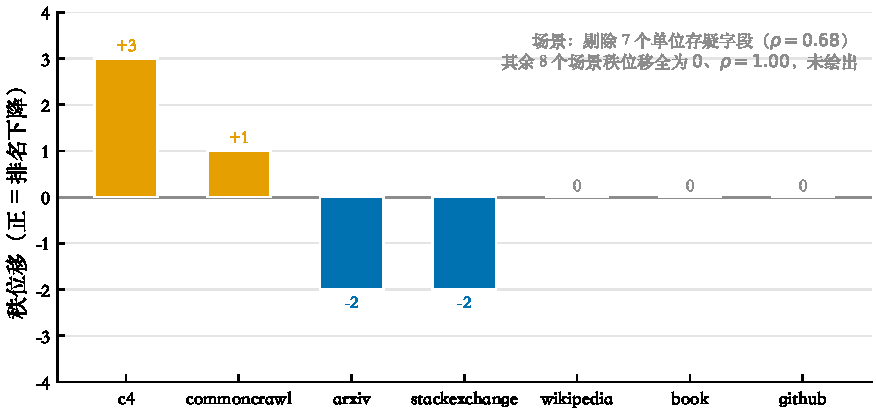
\includegraphics[width=.92\textwidth]{figures/q1-rank-robustness.pdf}
\caption{七域排序预处理稳健性}
\label{fig:q1-rank}
\end{figure}

\subsection{本章小结}

本问的三项交付如下。质量评分方面，22 个指标经 A1 单点校准的方向统一后合成两个
候选，等权候选的 A1 宏平均为 $0.49622$（$95\%$ 区间 $[0.49491,0.49763]$），稳定性
加权 Huber 候选为 $0.49848$（$[0.49657,0.50043]$），后者按接口一致性选为操作主分；
A2/A3 与 A1 的同域差值四个区间全部跨零，点估计均在千分位以下。冲突分析方面，22 个
指标构成 231 对，A1 各域的中位冲突度在 $0.2712$--$0.4382$ 之间，最高的指标对为
\texttt{dsir\_math} 与 \texttt{rps\_doc\_unigram\_\allowbreak entropy}（$0.5993$），
消解采用稳定性加权 Huber 位置。配比建模方面，单纯形岭回归在 A4/A5 交叉验证上以
$0.39860$ 略优于参考分量 OLS，同尺度检验集 A6/A7 的 $R^2=0.6189$、
Spearman $=0.8327$，136 个域对中 106 对有足够份额支持 10 个百分点替代。

本问的结论受三条限制约束。第一，$Q$ 是受限候选分：30 条小样本人工核查的评审间
一致性为 $\kappa=0.765$、Spearman $=0.806$，但该核查不能区分两个候选，故主分的
确定属接口一致性选择而非效度验证的胜出，793 条规模的全量人工评分未实施；另有 7 个
\texttt{rps\_*frac*} 字段的上游生成公式未追溯，整体剔除后 A1 样本分的 P95 绝对差达
$0.113048$，本文以该场景作为语义不确定性的上界探测。第二，配比模型不具备跨尺度
定量外推能力，60M 与 1B 上的 $R^2$ 转负（$-7.93$ 与 $-810.12$），Spearman 仍保持
$0.73$--$0.83$，可用的只是同尺度内的排序而非跨尺度预测。第三，配比域比损失目标
多 4 个，这 4 个域的损失不可观测，是模型的结构性限制。

本问交付给问题二的是质量评分 $Q$ 的可比尺度（$[0,1]$，A1 七域宏平均 $0.498478$，
版本 \texttt{Q1-q\_huber-v1}）与 17 维配比 $\pi$ 的单纯形定义，问题二须在此基础上
构造含 $N$、$D$、$Q$、$\pi$ 的广义标度律。
\clearpage
\section{问题二的模型建立与求解}

% ============================================================
% ⚠ 问题二的陷阱（U09--U12）
%   · 弹性必须是【无量纲】的 ε=(∂Loss/∂N)·(N/Loss)，
%     不是边际变化率 ΔLoss/ΔN（U10 明确诱导你"不用乘 N/L"）
%   · 参数【必须自己拟合】，不得采用任何预置数值（U11）
%   · 弹性的【符号必须自己检验】。Loss 随 N/D/Q 增大应【下降】，
%     若算出全为正号，先怀疑算错而不是写进论文（U12）
%   · 拟合不佳时不得靠加高次多项式硬凑（U09）
% ============================================================


\subsection{问题二分析}

本问要求把数据质量 $Q$ 与领域配比 $p$ 显式纳入标度律，在经典形式
$L(N,D)=E+AN^{-\alpha}+BD^{-\beta}$ 之外构造同时含 $N$、$D$、$Q$、$p$ 的广义关系，
并据此分析各因素的边际效用与弹性、讨论领域之间的替代与互补、推导质量提升与规模
扩大可相互替代的条件，最后完成参数估计与检验。按题目规定，附件 A 的信息经问题一
输出的 $Q$ 与 $p$ 引入，本问不重复读取 A 的原始文件；直接使用的数据为附件 B 的
B1--B12，其中 B11 与 B12 为辅助。问题一交付的 $Q$ 取值于 $[0,1]$，A1 七域宏平均为
$0.498478$；配比 $p$ 为 17 维单纯形向量（问题一记作 $\pi$，本问沿用题目记号 $p$）。

本问的真正困难不在拟合，而在识别。附件 A 与附件 B 是两组相互独立的实验，二者
都以交叉熵损失为可观测量，题目要求参赛队伍提出可检验的假设把两组规律统一到同一
模型中；换言之，"两组的 Loss 处于同一量尺"本身是一个必须检验的前提，而不是可以
默认的事实。同时，$Q$ 与 $p$ 在本数据上并非自由变化的两个变量：问题一的诊断已经
表明，依据配比派生出的质量特征是 $p$ 的确定性函数，若把它与 $p$ 并列放进回归，
形如 $p^{\top}b+\theta Q$ 的模型在 $p^{\top}(b+\theta\tilde Q)$ 的意义下不可分别
识别。配比一侧同样受限：附件 B 的各来源表中没有可逐行追溯到具体训练运行的 17 维
配比向量，因此 $p$ 的边际效应无法从 B 组数据直接估计。

本问的输出有三项，供问题三使用：经典分支的五个标度律参数及其不确定性、各因素的
弹性，以及质量基线的取值 $Q_0$。问题三在算力约束下分配资源时，$L$ 对 $N$、$D$ 的
响应取自本问冻结的参数，$Q$ 的提升成本与收益则以本问的弹性结构为参照。

本问的建模与验证是一个逐级放行的过程：经典形式先立住，配比与质量才依次尝试进入。
完整的判定路径与两道门禁的当前状态见图 \ref{fig:q2-flowscaling}。

\begin{figure}[htp!]
\centering
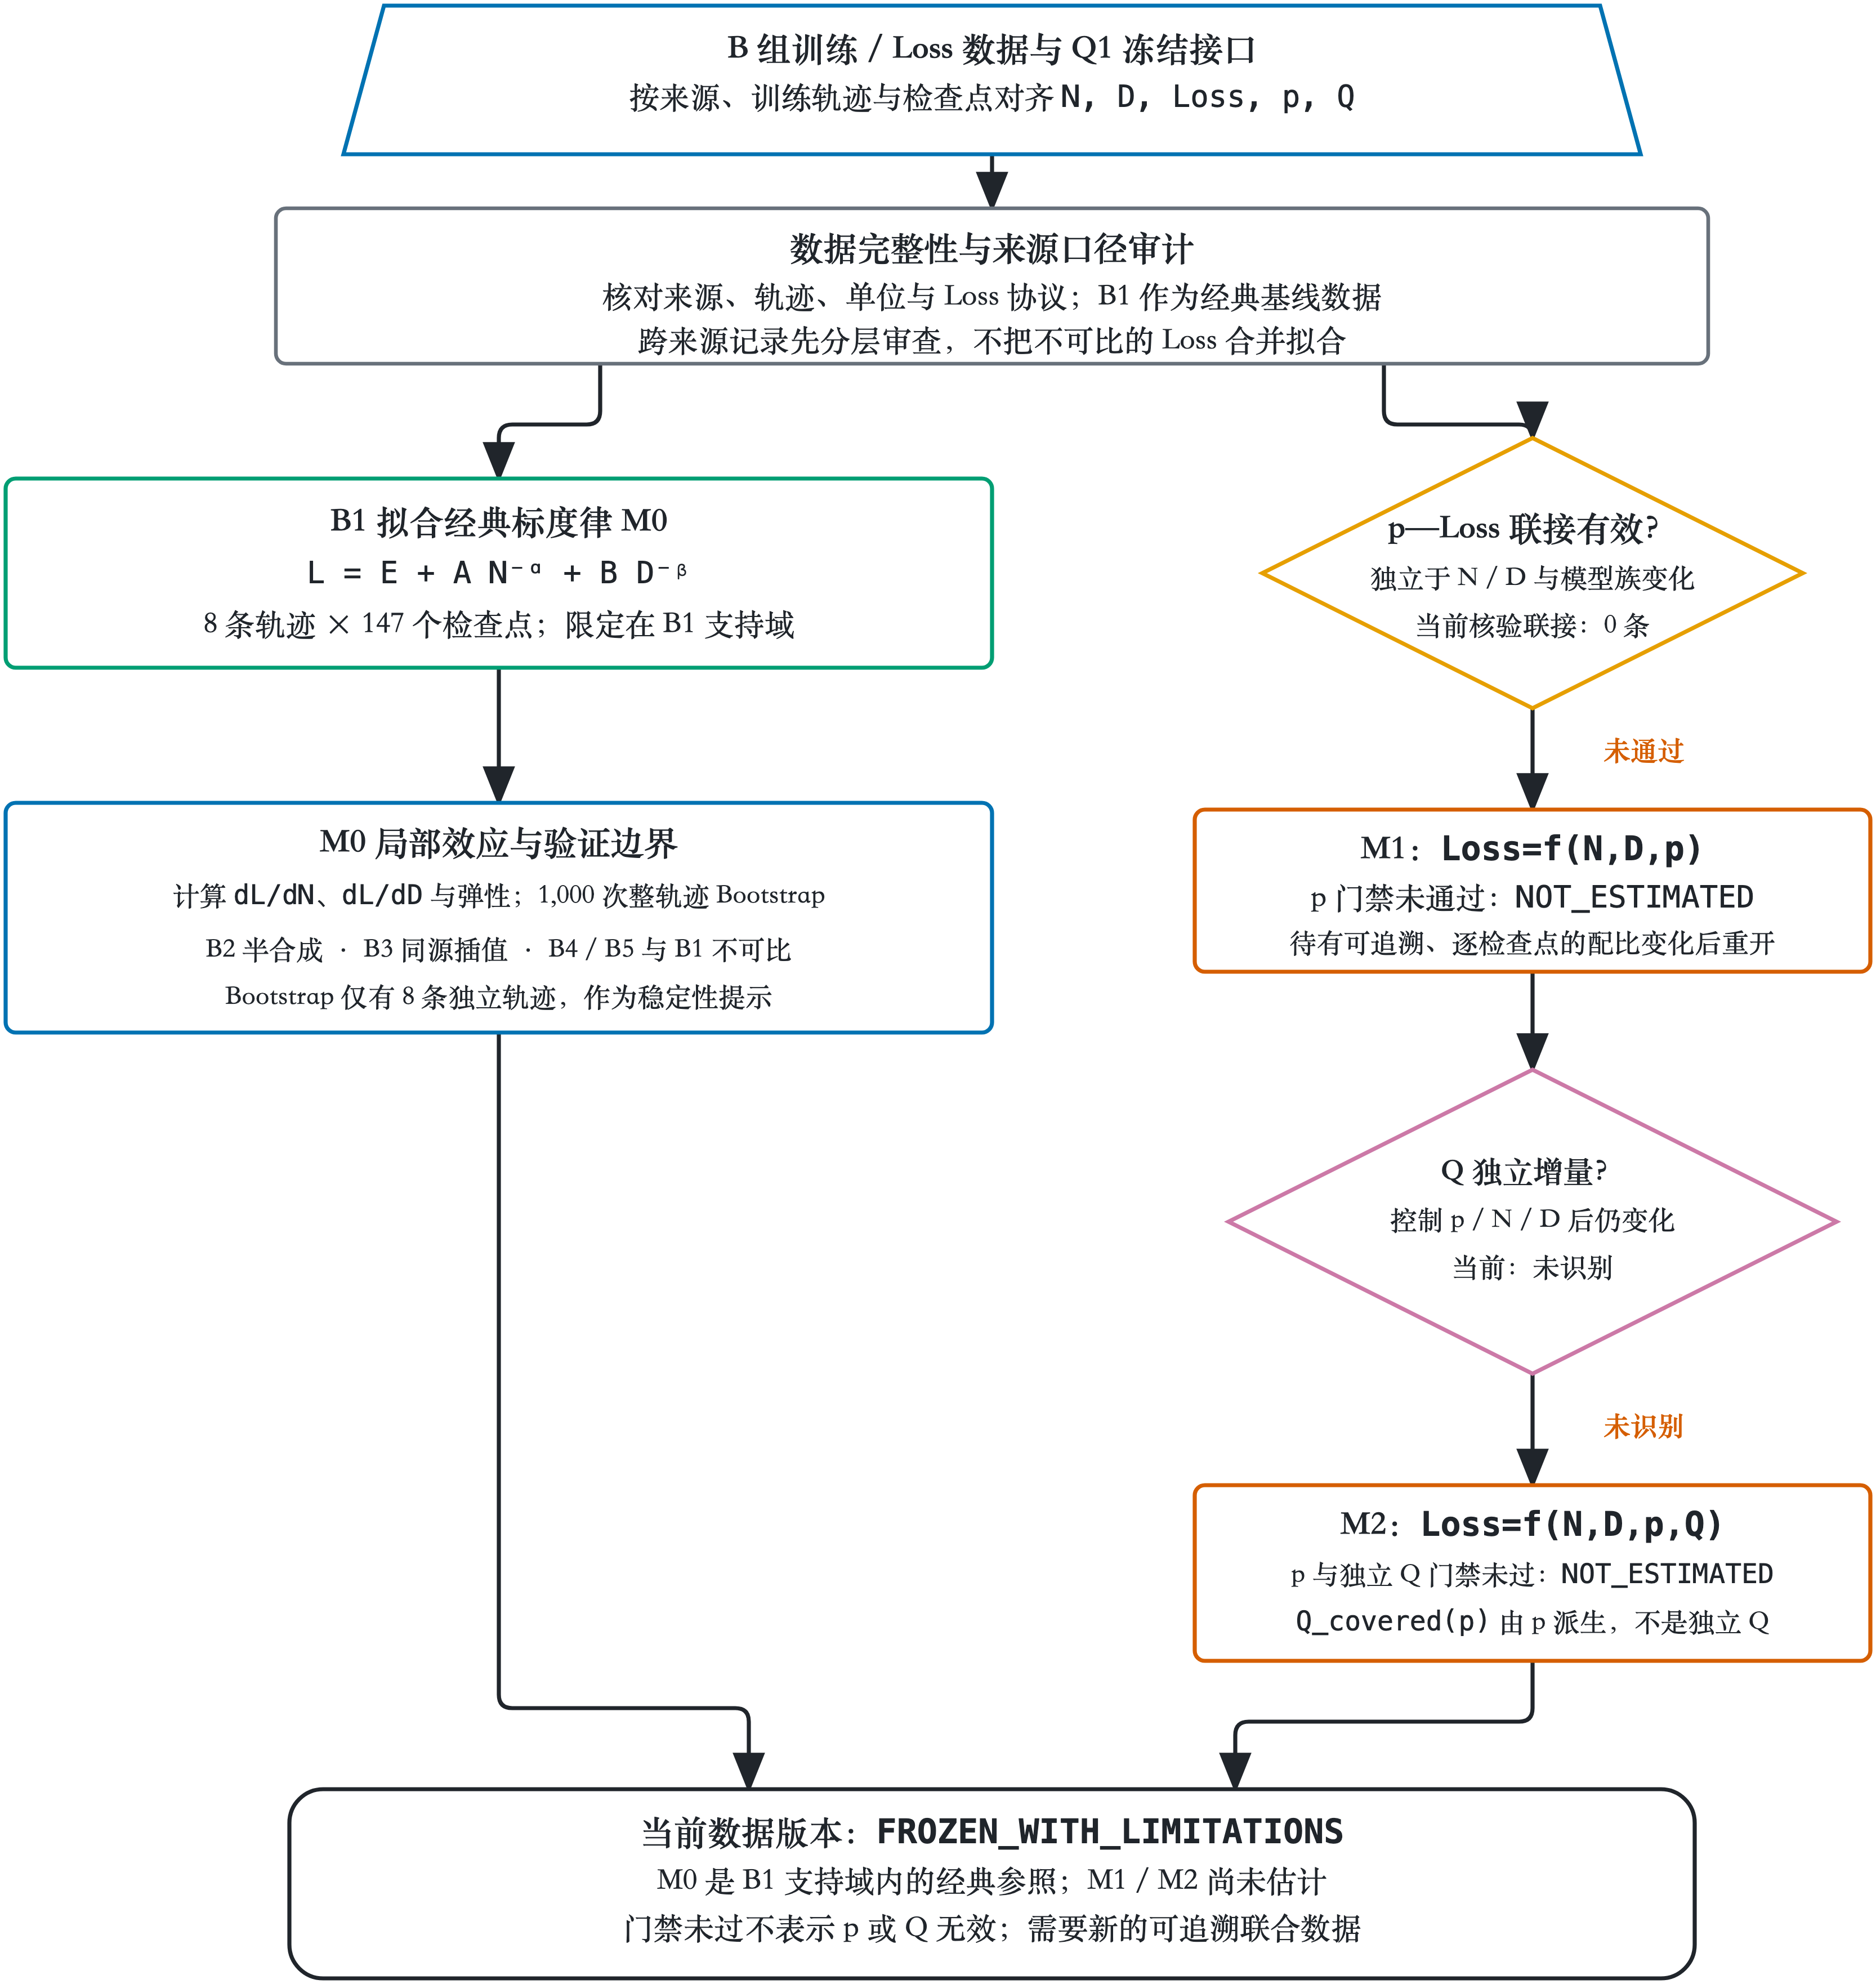
\includegraphics[width=\textwidth]{figures/q2-flow-scaling.png}
\caption{广义标度律建模路径}
\label{fig:q2-flowscaling}
\end{figure}

\subsection{模型建立}

\subsubsection{广义标度律的嵌套形式}

质量与配比对损失的作用通过"有效数据量"进入模型。记

\begin{equation}
L=E+A\,N^{-\alpha}+B\,D_{\mathrm{eff}}^{-\beta},\qquad
D_{\mathrm{eff}}=D\exp\{h(Q,p)\}
\end{equation}

式中，$E$ 为不可约损失，$A$ 与 $\alpha$ 刻画参数量方向的衰减，$B$ 与 $\beta$ 刻画
数据量方向的衰减，$D_{\mathrm{eff}}$ 为把数据质量与领域配比折算之后的等效数据量，
$h$ 为折算函数。对 $h$ 施加参考态约束

\begin{equation}
h(Q_{\mathrm{ref}},p_{\mathrm{ref}})=0
\end{equation}

使模型在参考状态处精确退化为经典形式。这条约束的作用是保证广义模型是经典的
严格扩展而非替换：当数据质量达到参考水平且配比取参考配方时，模型必须回到
$L=E+AN^{-\alpha}+BD^{-\beta}$，否则两套结果无法互相校验。取参考质量为
$Q_{\mathrm{ref}}=1$，则 $Q\to 1$ 时 $h\to 0$，模型退化为经典形式；这一退化是设计
出来的性质，不是拟合得到的实证结论。

$h$ 的分量按可识别性由少到多排列，构成同一族内的三个嵌套模型：

\begin{equation}
\text{M0}:\ h=0;\qquad
\text{M1}:\ h=g_p(p);\qquad
\text{M2}:\ h=g_p(p)+g_Q(Q)
\end{equation}

式中，M0 为经典参考分支，M1 在配比方向增加一个增量，M2 再叠加质量方向的增量。
嵌套的意义在于：只有当前一层已能识别，后一层的新增系数才有解释；若跳过 M1 直接
拟合 M2，则 $g_Q$ 吸收的可能是配比未能解释的部分，其系数不能读作质量效应。

考虑 $h$ 只含质量项的最简可拟合形式，取 $g_Q(Q)=\gamma\log Q$，此时
$D_{\mathrm{eff}}=D\,Q^{\gamma}$，模型化为

\begin{equation}
L=E+A\,N^{-\alpha}+B\,D^{-\beta}Q^{-\kappa},\qquad \kappa=\gamma\beta
\end{equation}

该形式在 $Q=1$ 处退化为经典形式，且弹性具有封闭表达式，便于后续推导替代条件。
本文在附件 B 的质量数据上估计这一形式，其证据等级见 \ref{sec:q2-sens}。

\subsubsection{边际效应与弹性的定义}

题目要求分析各因素的边际效用与弹性，二者不是同一个量。边际效用是损失对自变量的
偏导数，带量纲；弹性是无量纲的相对变化率：

\begin{equation}
\frac{\partial L}{\partial x}
=\begin{cases}
-\alpha A\,N^{-\alpha-1}, & x=N\\[2pt]
-\beta B\,D^{-\beta-1}Q^{-\kappa}, & x=D\\[2pt]
-\kappa B\,D^{-\beta}Q^{-\kappa-1}, & x=Q
\end{cases}
\qquad
\varepsilon_x=\frac{\partial L}{\partial x}\cdot\frac{x}{L}
\end{equation}

式中，$\varepsilon_x$ 为因素 $x$ 的弹性，含义是 $x$ 增加 $1\%$ 时 $L$ 变化的百分比。
采用无量纲弹性而非边际导数的理由有二：其一，$N$、$D$、$Q$ 的量纲与量级完全不同，
边际导数之间不可直接比较，无法回答"同样多花一块钱投在哪一项更划算"；其二，题目
要求推导质量与规模可相互替代的条件，而替代关系由等损失曲线给出，其斜率正是两个
边际导数之比，用弹性表达才具有跨量级的可比性。$L$ 随 $N$、$D$、$Q$ 增大应单调
下降，故三个弹性在参数为正时应全为负号；符号若为正，应先怀疑计算有误。

由等损失条件可直接得到替代关系。令 $\mathrm{d}L=0$，在固定 $D$ 的条件下有

\begin{equation}
\left.\frac{\mathrm{d}N}{\mathrm{d}Q}\right|_{L}
=-\frac{\partial L/\partial Q}{\partial L/\partial N}
=-\frac{\kappa\,N}{\alpha\,Q}\cdot\frac{AN^{-\alpha}}{BD^{-\beta}Q^{-\kappa}}
\end{equation}

式中，右端第一个因子是弹性的比值，第二个因子是两个衰减项之比。该式给出"质量提高
一个单位需要以多少参数量作为代价"的连续形式，其数值含义在 \ref{sec:q2-result} 中
以有限增量的方式报告。

\subsection{模型求解}

求解分四步：数据审计、参数估计、不确定性量化与外推检验。数据审计先行，用于确认
各附件在本次建模中的角色与支持范围，避免把同名但不可比的记录混入拟合。审计覆盖
输入文件清单、角色契约、轨迹映射与设计支持四项，共 36 项检查全部通过。B1 共
1176 行，按 B12 的检查点索引映射为 8 条完整的 Pythia 训练轨迹，每条轨迹
147 个检查点；配比列在 B1 中为空。这里必须强调，1176 是检查点数而非独立实验数，
8 条轨迹才是独立的抽样单元，后续所有区间估计均按轨迹整簇重抽样。

参数估计在 B1 上用有界非线性最小二乘完成，约束为 $0\le E<\min(\mathrm{val\_loss})$
与 $A,\alpha,B,\beta>0$。为避免陷入局部极小，取 24 组固定初值做多重启动，以目标
函数最小的解为最终估计。不确定性用整轨迹整簇 bootstrap 量化：每次有放回地
从 8 条完整轨迹中抽取 8 条，保留其全部 147 个检查点后重新拟合，重复 1000 次。
按整簇而非按行重抽样是必要的，因为同一轨迹内相邻检查点的损失高度相关，按行抽样
会把序列相关误当作独立信息，从而严重低估区间宽度。外推检验采用留一规模法：每次
留出一条完整的 147 点轨迹，用其余 7 条重新拟合后预测被留出的轨迹。B1 的设计支撑
见图 \ref{fig:q2-support}：8 个参数量取值与 147 个训练检查点构成交叉设计，同一
$D$ 网格在各 $N$ 列之间水平对齐，这正是 $\alpha$ 与 $\beta$ 能够分别识别、且缩放
雅可比条件数只有 $56.378$ 的原因；图中同时给出了该拟合所依赖的支持边界
（$N\le11.965825$B、$D\le299.893$B），后文讨论 B9/B10 外推时反复引用这两个上界。
求解步骤见表 \ref{alg:q2-solve}。

\begin{table}[htp!]
\centering
\renewcommand\arraystretch{1.2}
\caption{经典标度律的参数估计与不确定性量化步骤}\label{alg:q2-solve}
\begin{tabularx}{\textwidth}{cX}
\toprule
步骤 & 操作 \\
\midrule
1 & 审计附件角色与支持域，确认 B1 为唯一拟合数据、B2--B5 为验证数据 \\
2 & 按 B12 检查点索引把 B1 的 1176 行映射为 8 条完整轨迹 \\
3 & \textbf{for} 24 组固定初值 \textbf{do} 有界非线性最小二乘，记录目标函数值 \\
4 & 取目标函数最小的解为冻结参数 $\hat E,\hat A,\hat\alpha,\hat B,\hat\beta$ \\
5 & \textbf{for} $b=1$ \textbf{to} 1000 \textbf{do} 按轨迹整簇重抽样并重新拟合 \\
6 & 由 1000 组重抽样解取百分位区间，得各参数的 $95\%$ 区间 \\
7 & \textbf{for} 每条轨迹 \textbf{do} 留出该轨迹全部 147 点，用其余轨迹重拟合并预测 \\
8 & 在 B2--B5 上按来源分别计算误差，不合并、不重调参 \\
\bottomrule
\end{tabularx}
\end{table}

\begin{figure}[htp!]
\centering
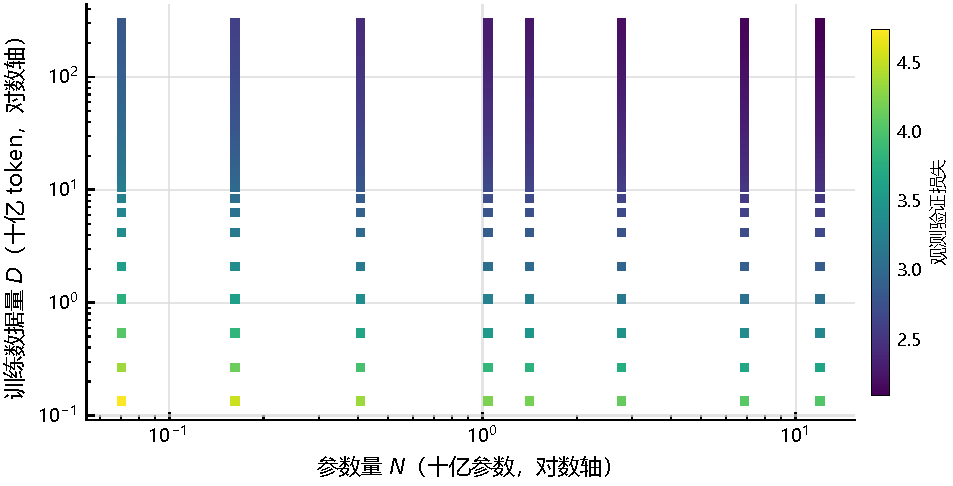
\includegraphics[width=.88\textwidth]{figures/q2-b1-support.pdf}
\caption{B1 标度律拟合支撑域}
\label{fig:q2-support}
\end{figure}

\subsection{结果分析}\label{sec:q2-result}

\subsubsection{经典分支的参数与拟合优度}

经典分支 M0 的参数估计与区间见表 \ref{tab:q2-params}。五个参数在 1000 次整轨迹
bootstrap 下的区间都很窄，这是 8 条轨迹所覆盖的 $N$、$D$ 跨度较宽、且设计点近似
正交的直接结果；但区间的可靠性受簇数限制，只能作为稳定性提示（见
\ref{sec:q2-sens}）。

\begin{table}[htp!]
\centering
\renewcommand\arraystretch{1.2}
\caption{B1 经典标度律参数估计}\label{tab:q2-params}
\begin{tabular*}{\textwidth}{@{\extracolsep{\fill}}lccc@{}}
\toprule
参数 & 估计值 & $95\%$ 区间下界 & $95\%$ 区间上界 \\
\midrule
$E$     & 1.689798 & 1.689645 & 1.689962 \\
$A$     & 0.353980 & 0.353843 & 0.354125 \\
$\alpha$& 0.339977 & 0.339831 & 0.340115 \\
$B$     & 1.240306 & 1.240160 & 1.240434 \\
$\beta$ & 0.279878 & 0.279823 & 0.279937 \\
\bottomrule
\end{tabular*}
\end{table}

拟合在 1176 个检查点上的内样本指标为：RMSE $=1.4650\times10^{-4}$，MAE
$=1.0523\times10^{-4}$，最大绝对误差 $=9.2038\times10^{-4}$，$R^2=0.99999982$，
Spearman $=0.99999965$。缩放雅可比矩阵满秩（$5/5$），条件数为 $56.378$，远低于
病态告警阈值，说明五个参数在该设计下不存在共线退化；24 组初值全部收敛，最优解
之间的最大相对参数跨度为 $4.46\times10^{-10}$，可排除初值敏感性。需要明确的是，
这些是拟合内指标，$R^2$ 接近 1 只说明经典形式在 B1 支持域内能忠实描述损失随
$N$、$D$ 的变化，不构成模型正确性的外部证据；外部证据由 \ref{sec:q2-sens} 的
分来源验证承担。

留一规模检验的结果同样紧凑：留出 12B 轨迹时 RMSE 为 $1.0198\times10^{-4}$，留出
70m 轨迹时为 $2.2023\times10^{-4}$，八条轨迹的留出 $R^2$ 介于 $0.99999923$ 与
$0.99999983$ 之间，秩相关均为 $1.0000$。误差在小规模端更大，这与幂律模型在小
$N$ 端曲率更强的特性一致。

拟合优度接近 1 的数值应当有对应的诊断支撑，否则读者无从判断残差是否只被均值
掩盖。图 \ref{fig:q2-residual} 给出残差对拟合值的散布：残差均值为
$+2.6\times10^{-14}$，即经典形式不存在系统性偏倚；残差标准差为
$1.47\times10^{-4}$。但残差的离散程度随损失水平上升而扩大——拟合值在 2.0 至 2.5
之间的 760 个点几乎全部落在 $\pm2\times10^{-4}$ 以内（极值 $\pm3.8\times10^{-4}$），
拟合值超过 3.0 的 58 个点则扩展到 $[-6.5\times10^{-4},+9.2\times10^{-4}]$。全样本
只有 1 个点的绝对残差超过 $7\times10^{-4}$。这是异方差而非偏倚：它不否定参数的
估计，但提示该模型的误差并非同分布。这一点在问题三按预算筛选候选点时不影响排序，
因为筛选依据的是预测值本身而非区间宽度。

\begin{figure}[htp!]
\centering
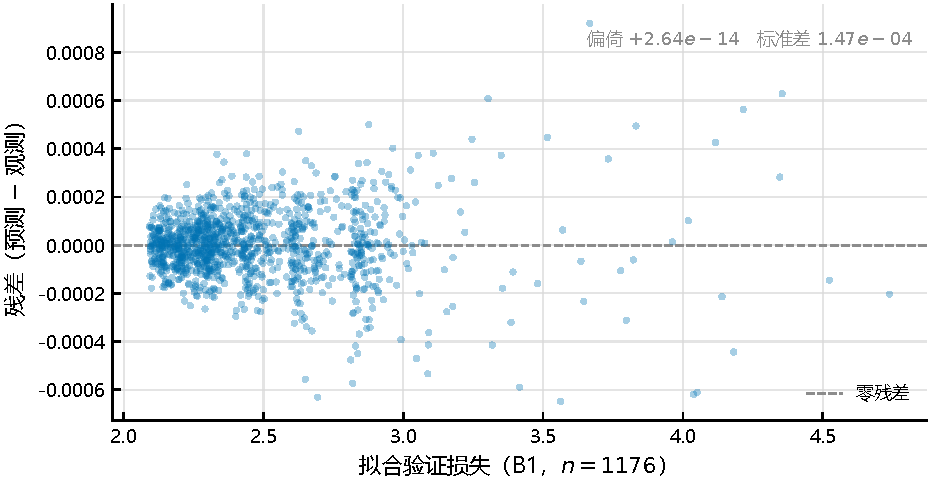
\includegraphics[width=.92\textwidth]{figures/q2-b1-residual.pdf}
\caption{B1 标度律残差结构}
\label{fig:q2-residual}
\end{figure}

\subsubsection{边际效应与弹性}

在 B1 的中位点（$N=1.2285$B 参数、$D=146.80$B token，预测损失 $2.3268$）处，
各因素的边际效应与弹性为：

\begin{table}[htp!]
\centering
\renewcommand\arraystretch{1.2}
\caption{B1 中位点边际效应与弹性}\label{tab:q2-elas}
\begin{tabular*}{\textwidth}{@{\extracolsep{\fill}}llcc@{}}
\toprule
因素 & 量纲 & 边际效应 $\partial L/\partial x$ & 弹性 $\varepsilon_x$ \\
\midrule
参数量 $N$ & 每 $+1$B 参数 & $-0.091339$ & $-0.048225$ \\
数据量 $D$ & 每 $+1$B token & $-5.8526\times10^{-4}$ & $-0.036924$ \\
\bottomrule
\end{tabular*}
\end{table}

两个弹性均为负，与"损失随规模增大而下降"的先验方向一致。数值上，参数量的弹性
绝对值略大于数据量（$0.0482$ 对 $0.0369$），即在该工作点上增加同等百分比参数量
带来的损失下降更多。这一比较必须限定在中位点附近：弹性本身随工作点移动，不是
常数。

逐规模的弹性见表 \ref{tab:q2-elas-size}，其中 $\varepsilon_N$ 与 $\varepsilon_D$
呈现方向相反的趋势。

\begin{table}[htp!]
\centering
\renewcommand\arraystretch{1.2}
\caption{八条轨迹的 N 弹性与 D 弹性中位数}\label{tab:q2-elas-size}
\begin{tabular*}{\textwidth}{@{\extracolsep{\fill}}lccccccc@{}}
\toprule
模型规模 & 70m & 160m & 410m & 1b & 1.4b & 2.8b & 6.9b \\
\midrule
$\varepsilon_N$ & $-0.1033$ & $-0.0841$ & $-0.0659$ & $-0.0506$ & $-0.0463$ & $-0.0378$ & $-0.0287$ \\
$\varepsilon_D$ & $-0.0300$ & $-0.0324$ & $-0.0347$ & $-0.0366$ & $-0.0372$ & $-0.0382$ & $-0.0394$ \\
\bottomrule
\end{tabular*}

\vspace{2pt}
\begin{tabular*}{\textwidth}{@{\extracolsep{\fill}}lcc@{}}
\toprule
模型规模 & 12b & 极差 \\
\midrule
$\varepsilon_N$ & $-0.0241$ & $[-0.1033,\,-0.0241]$ \\
$\varepsilon_D$ & $-0.0400$ & $[-0.0400,\,-0.0300]$ \\
\bottomrule
\end{tabular*}
\end{table}

$\varepsilon_N$ 从 70m 处的 $-0.1033$ 单调减弱到 12b 处的 $-0.0241$，即模型越大，
参数量翻倍带来的相对收益越小；$\varepsilon_D$ 则从 $-0.0300$ 增强到 $-0.0400$。
两条曲线在中段（约 1b 附近）交叉。这一结构提示：在小规模端扩大参数量更有效，在
大规模端继续增加训练数据的相对回报更高，与 Chinchilla 关于"参数量与数据量应
同比例增长"的经验结论方向一致，但本文给的是同一模型族内的连续弹性和交叉位置，
而非最优配比本身。边际效应 $\partial L/\partial D$ 在相同的 $D$ 处八条轨迹取值
完全相同——因为 M0 形式中该项只依赖 $D$ 而不依赖 $N$，这是该函数形式的结构性含义
而非拟合巧合；但必须注意它并非随 $D$ 不变：沿单条轨迹，该量从 $D$ 最小处的
$-4.5467$ 变到 $D$ 最大处的 $-2.35\times10^{-4}$，跨约四个数量级，表中引用的
$-5.8526\times10^{-4}$ 是轨迹中位数而非全轨迹常数。

比较两个弹性的变化来源时可以看到一个不对称：$\varepsilon_D$ 沿单条轨迹随训练
推进的跨度（p10 至 p90）达 $0.1142$，而八条轨迹的中位数之间只相差 $0.0100$，
相差一个量级。也就是说，$D$ 弹性的主要变化来自"训练进行到哪一步"，而不是"模型
有多大"；前者在图 \ref{fig:q2-elasticity} 的面板 (b) 中体现为灰棒的长度，后者只
表现为八个点位的水平位移。这一区分对问题三有直接含义：在预算分配中若把
$\varepsilon_D$ 当作与训练进度无关的常数使用，会引入远大于规模间差异的误差。

边际效应与弹性的完整轨迹见图 \ref{fig:q2-marginal} 与 \ref{fig:q2-elasticity}。
两图中的区间均来自问题二的 1000 次整轨迹 bootstrap；其中 $|\partial L/\partial D|$
的区间半宽最大不足坐标跨度的 $0.1\%$，在纸面上窄于线宽，故未单独填色绘出，
改以文字标注，以免留下一条读者看不见的置信带。无量纲弹性图的上排展示全尺度趋势及
轨迹内 p10--p90 跨度，下排单独放大整轨迹 bootstrap 区间；两条区间带分别只占纵轴跨度
的 $0.07\%$ 与 $0.14\%$，因此在全尺度面板中窄于线宽。

\begin{figure}[htp!]
\centering
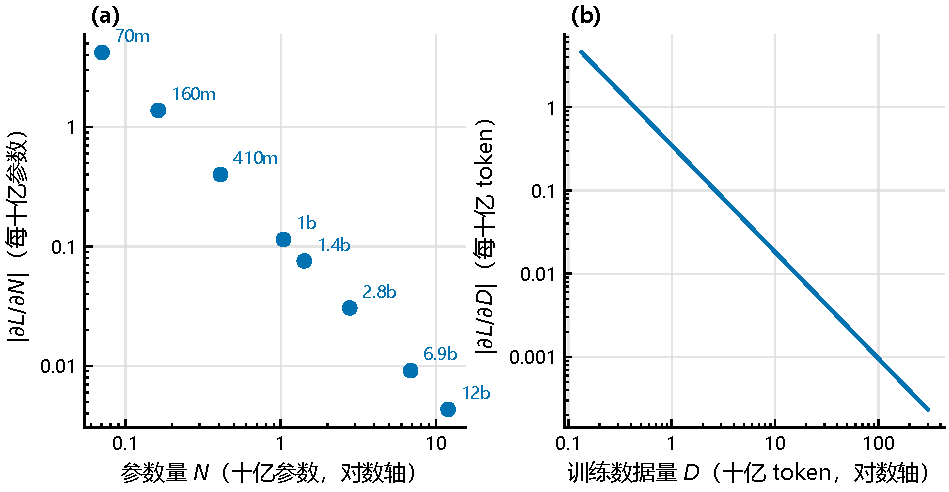
\includegraphics[width=.94\textwidth]{figures/q2-m0-marginal.pdf}
\caption{规模与数据量的边际效应}
\label{fig:q2-marginal}
\end{figure}

\begin{figure}[htp!]
\centering
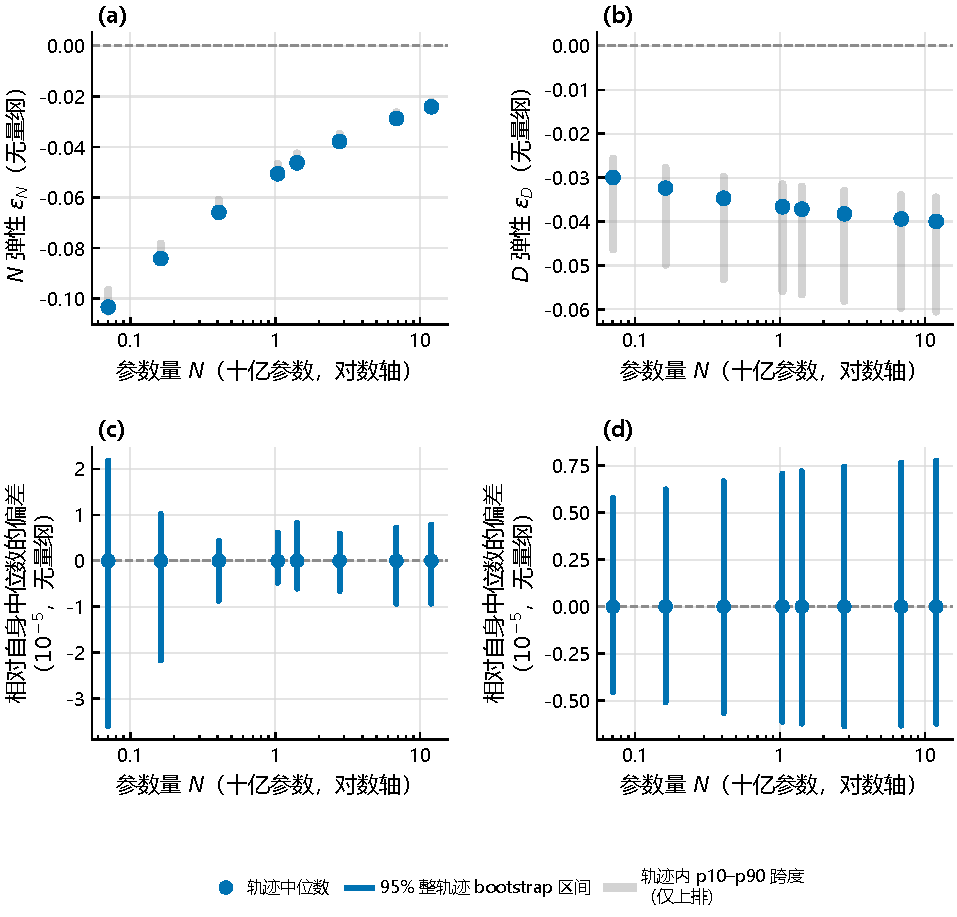
\includegraphics[width=.94\textwidth]{figures/q2-m0-elasticity.pdf}
\caption{训练轨迹上的无量纲弹性}
\label{fig:q2-elasticity}
\end{figure}

上两图把弹性汇总到规模这一维，看不到它在单条轨迹内随训练推进的完整形状。
图 \ref{fig:q2-elasticity-profile} 按 $N$ 分面给出两个弹性沿 $D$ 的剖面，每个
主图下方另附一条放大窄条，把 $95\%$ 区间相对估计值的偏差按其真实尺度展开。剖面
显示出两点汇总图看不到的结构：其一，两个弹性随 $D$ 单调变化且八个规模上的形状
一致，说明这种依赖来自 M0 的函数形式而非某个规模的偶然；其二，$\varepsilon_D$ 的
区间带在小 $D$ 端明显张开、随 $D$ 增大而收拢，即训练token越多，该弹性的估计越
稳定。需要与图 \ref{fig:q2-elasticity} 并读：后者画的是逐轨迹中位数与 p10--p90
跨度，前者画的是沿 $D$ 的完整曲线，因此前者在小 $D$ 端会低到后者 p10 以下——
两者口径不同，不是相互矛盾。剖面区间基于 8 条完整 Pythia 轨迹，只作重抽样稳定性
提示；曲线是冻结 M0 的函数蕴含量，不代表配比或质量效应。

\begin{figure}[htp!]
\centering
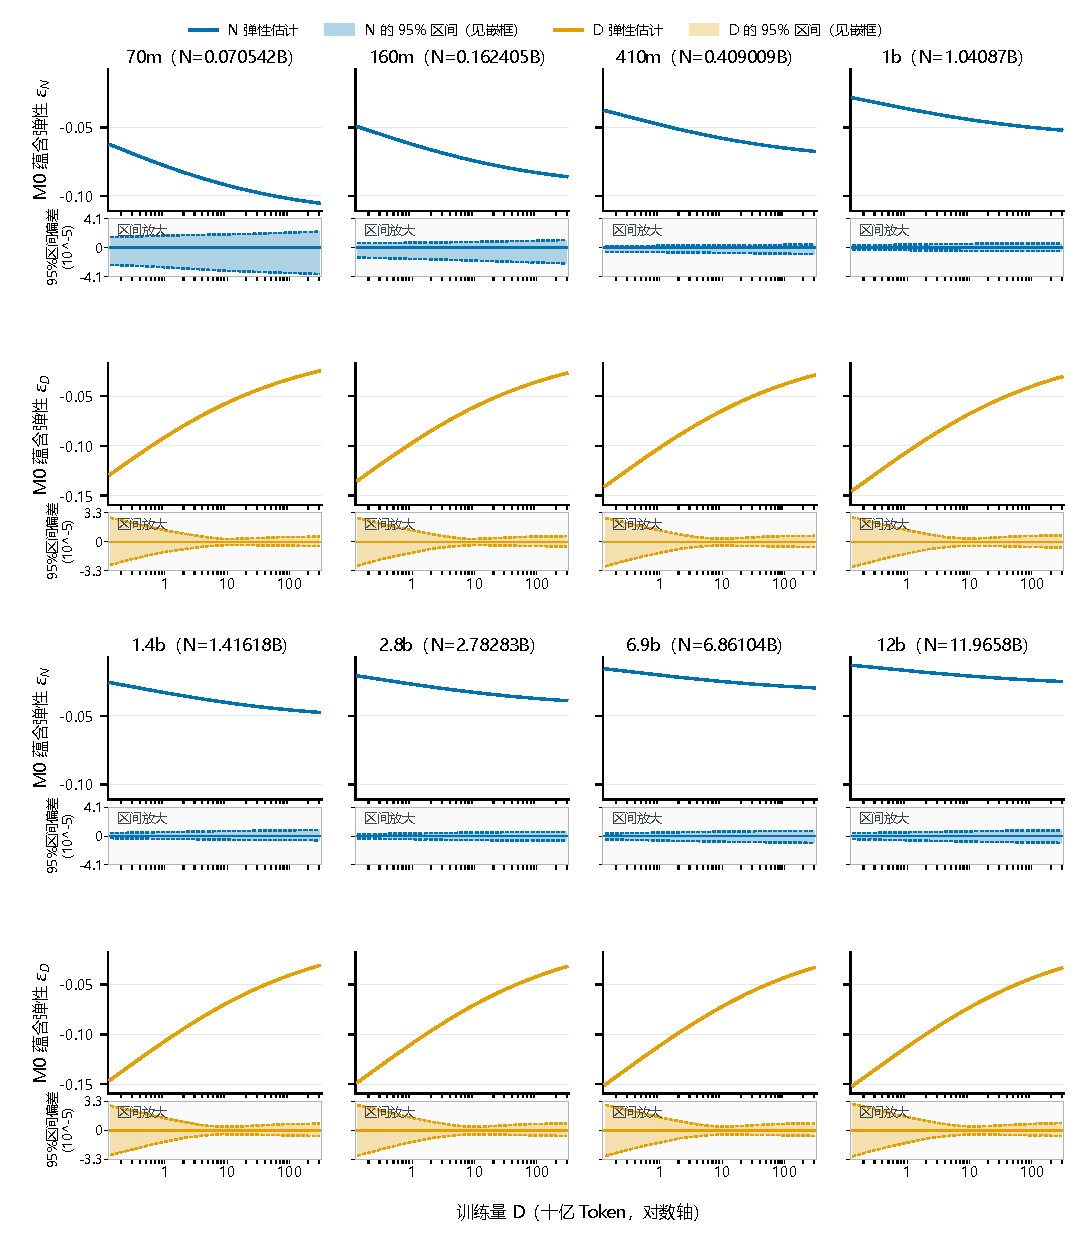
\includegraphics[width=\textwidth]{figures/q2-elasticity-profile.pdf}
\caption{冻结 M0 下的弹性剖面}
\label{fig:q2-elasticity-profile}
\end{figure}

\subsubsection{质量与规模的等损失兑换条件}

题目要求回答"质量提升 $0.1$ 等价于参数增加多少"。该条件在 $h=g_Q(Q)=\gamma\log Q$
的设定下可直接由 \ref{sec:q2-result} 的等损失关系解出。用于估计 $Q$ 方向的系数时，
附件 B 中只有 B6 与 B7 含有质量维度，且二者按《数据说明》均为基于真实标度律校准
并叠加噪声的半合成数据，不是直接实验观测。在这两组数据上拟合
$L=E+AN^{-\alpha}+BD^{-\beta}Q^{-\kappa}$，得

\begin{table}[htp!]
\centering
\renewcommand\arraystretch{1.2}
\caption{半合成数据的质量指数估计}\label{tab:q2-qfit}
\begin{tabular*}{\textwidth}{@{\extracolsep{\fill}}lccccccc@{}}
\toprule
数据集 & 行数 & $\kappa$ & $\gamma=\kappa/\beta$ & $\varepsilon_Q$ 中位数 & 不含质量项 & 含质量项 & 相对改善 \\
\midrule
B6 & 360 & 0.085033 & 1.216453 & $-0.054048$ & 0.145135 & 0.089840 & $38.1\%$ \\
B7 & 450 & 0.098000 & 1.179775 & $-0.052055$ & 0.129540 & 0.084316 & $34.9\%$ \\
\bottomrule
\end{tabular*}
\end{table}

式中，"不含质量项"与"含质量项"两列为同一半合成网格上 $M0$ 与 $M_Q$ 两个模型的
留一 Q 水平 RMSE，"相对改善"为二者之差相对前者的比例。含质量项的模型误差在两个
数据集上分别低 $38.1\%$ 与 $34.9\%$，说明半合成网格确实携带了 $Q$ 方向的信号。
取共同网格中心（$N=1$B、$D=150$B、$Q=0.6$）为工作点，把 $Q$ 提高 $0.1$
后维持损失不变所需的参数量为

\begin{table}[htp!]
\centering
\renewcommand\arraystretch{1.2}
\caption{质量提升的等损失参数量兑换}\label{tab:q2-trade}
\begin{tabular*}{\textwidth}{@{\extracolsep{\fill}}lccc@{}}
\toprule
数据集 & 兑换前的 $N$ & 兑换后的 $N$ & 参数量变化 $\Delta N$ \\
\midrule
B6 & 1.000000B & 0.878085B & $-0.121915$B \\
B7 & 1.000000B & 0.881795B & $-0.118205$B \\
\bottomrule
\end{tabular*}
\end{table}

即在给定的工作点上，质量评分每提高 $0.1$，可替代约 $0.12$B 参数量，相当于原参数
量的 $12\%$。方向与量级在两组半合成数据上一致（$-0.1219$B 与 $-0.1182$B），这是
该结论中唯一可比对的一致性证据。

该数值的解释必须限定在四重边界之内。其一，它来自半合成拟合曲面，是对照数据
说明允许的补充分析，不能表述为真实训练观测，也不是实际训练中的资源替代率。其二，
它衡量的是等损失关系而非等算力或等成本关系——提高质量本身需要额外算力，该
成本由问题三的成本函数处理，本处未计入。其三，$Q$ 在 B6/B7 中是半合成网格自带的
评分列，其量尺与问题一交付的 $Q$ 是否一致尚无证据，故 $-0.12$B 这一兑换率不能
直接叠加到问题一的 $Q$ 刻度上使用。其四，B7 与 B6 的重合部分为 360/360 行且损失
改动为零，二者不是独立重复实验；另一份含质量维度的 B8 在固定 $N$、$D$ 后与 B6/B7
方向相反，在未取得可验证的生成规则之前本文不把三份数据合并估计单一质量弹性。
因此本表只作为条件性示例报告，不进入任何后续优化目标。

这一方向冲突不宜只以文字断言，其图证见图 \ref{fig:q2-qsign}。在控制了 $N$ 与 $D$
的匹配单元内逐单元估计 Loss 对 $Q$ 的斜率，B6 的 45 个单元与 B7 的 45 个单元
全部为负，而 B8 的校准部分 90 个单元与 外推部分 60 个单元全部为正，无一例外；
两个方向的中位斜率分别为 $-0.3409$、$-0.3393$ 与 $+2.0279$、$+1.8105$，池化
Spearman 相关为 $-0.324$、$-0.299$ 与 $+0.933$、$+0.966$。符号完全分离意味着这
不是噪声导致的方向不定，而是两组数据在生成层面就不同——这正是本文坚持不合并
估计、并把质量弹性限定为条件性示例的直接理由。

\begin{figure}[htp!]
\centering
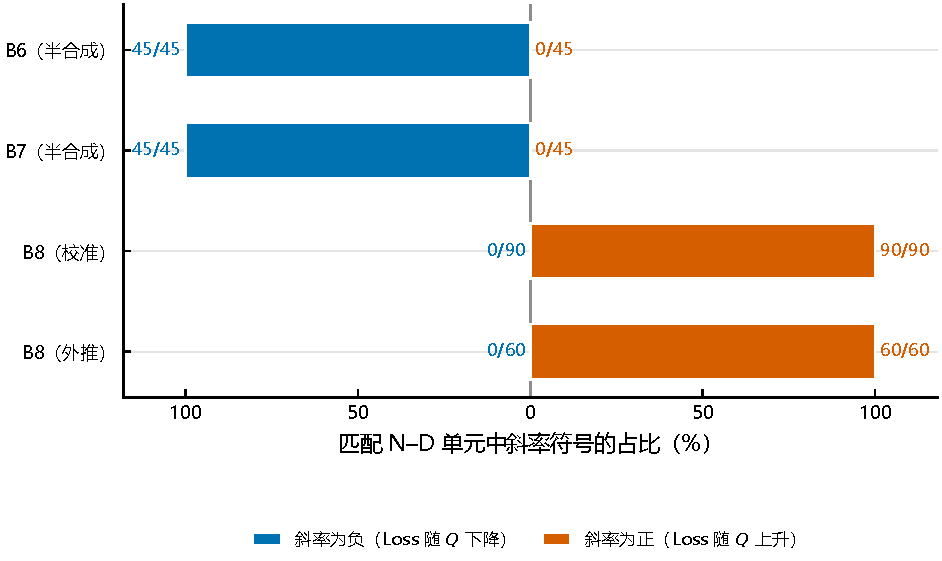
\includegraphics[width=.90\textwidth]{figures/q2-q-sign.pdf}
\caption{质量指数斜率符号分布}
\label{fig:q2-qsign}
\end{figure}

\subsubsection{领域配比之间的替代与互补}

题目要求讨论不同领域数据之间的替代或互补关系。这一关系须在配比空间上定义，而不能
用相关系数代替，因为配比受单纯形约束，任一分量的增减都伴随其他分量的反向调整。
本文采用沿单纯形边的转移参数化：从一个基准配方 $p$ 出发，把 $\delta$ 的份额从
域 $j$ 转移到域 $i$，

\begin{equation}
p(\delta)=p+\delta\,(e_i-e_j),\qquad -p_i\le\delta\le p_j
\end{equation}

式中，$e_i$ 为第 $i$ 个坐标的单位向量，$\delta$ 为转移份额，其上下界保证转移后
各分量仍非负。在 $h(Q,p)$ 只含配比项的一阶近似下，单次转移对损失的局部影响为
$-\beta T\,[h_{p_i}-h_{p_j}]$，其中 $T=B\,D_{\mathrm{eff}}^{-\beta}$。

两个转移是否互补，由二阶交叉效应判定。记两个转移分别沿 $u$ 与 $v$ 方向，则

\begin{equation}
\Delta_u\Delta_v L
=T\bigl[\beta^2 (D_uh)(D_vh)-\beta\,D_uD_vh\bigr]
\end{equation}

式中，$D_u h$ 与 $D_v h$ 为一阶方向导数，$D_uD_vh$ 为二阶交叉导数。括号内第一项
恒非负，第二项取决于 $h$ 的曲率。约定 $\Delta_u\Delta_vL<0$ 为互补——两者同时
实施比分别实施多降损失；$>0$ 为替代——边际收益递减。需要说明，本文所用的二次面
敏感性模型的交叉曲率是模型设定的产物，线性主模型的该曲率恒为零，因此下面报告的是
二次模型下的探索性诊断，而不是数据证明的领域互补性。

在 A4/A5 的 512 条闭合配方上，以 500 次配方组 bootstrap 逐对估计，共得到 6551 个
联合可行的转移对：

\begin{table}[htp!]
\centering
\renewcommand\arraystretch{1.2}
\caption{A4/A5 上转移对的互补与替代方向统计}\label{tab:q2-compl}
\begin{tabular*}{\textwidth}{@{\extracolsep{\fill}}lccc@{}}
\toprule
判据 & 互补（区间全负） & 替代（区间全正） & 跨零 \\
\midrule
逐点 $95\%$ 区间（未校正） & 273 & 445 & 5833 \\
$\max|t|$ 家族校正后 & 0 & 39 & 6512 \\
\bottomrule
\end{tabular*}
\end{table}

按点估计计，6551 对中互补 3310 对、替代 3241 对，几乎均分。但这一均分在考虑抽样
不确定性后并不成立：逐点区间下已有 5833 对跨零，而施加 $\max|t|$ 家族校正
（临界值 $6.5403$）后，互补方向一对都不剩，仅 39 对保持替代方向。校正前的
候选集由全样本拟合的模型筛出，$\max|t|$ 只对已筛出的候选作近似单步校正，并不校正
筛选本身，因此这仍不是独立确认性检验。结论是：在本数据上未能识别出稳健的领域
互补关系；可用的供体域为 \texttt{arxiv}、\texttt{pubmed\_central}、\texttt{github}
与 \texttt{pile\_cc}，其余域的份额不足以支持 10 个百分点的转移。

这些结果限定在 A4/A5 来源内，与 B 侧无关。第 5 章的替代效应分析给出的是逐对区间的
方向计数，本节给的是二阶交叉效应与家族校正后的结论，两者互补而非重复。

\begin{figure}[htp!]
\centering
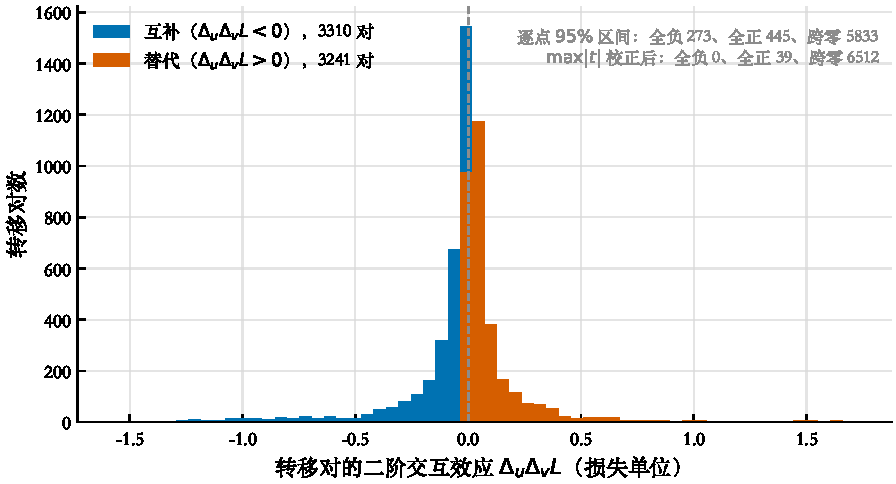
\includegraphics[width=\textwidth]{figures/q2-compl-dist.pdf}
\caption{配比转移的二阶交互效应}
\label{fig:q2-compl}
\end{figure}

\subsubsection{大尺度外推情景}

题目要求结合 B9、B10 讨论百亿参数以上的外推。B10 为按已拟合标度律估算的损失
表，不是独立观测，其 128 行模型的参数量全部超出 B1 的支持上界（$11.965825$B），
其中 102 行的数据量也超出 B1 的 $D$ 支持上界（$299.893$B）。把冻结的 M0 参数直接
代入 B10 的 $N$、$D$，得预测损失中位数 $1.90642$，范围
$[1.78384,4.08630]$；把 1000 组 bootstrap 参数逐一代入，区间的中位宽度仅
$1.590\times10^{-4}$。区间的窄是参数不确定性小的结果，不表示外推可靠：该
区间只传播了参数变异，未包含跨评测协议的损失偏差、模型形式错设与远距离外推误差。
偏差最大的几行集中在数据量极小的一端（如 $D=0.1$B），属于 B1 支持域外的低端
外推。因此本节只用于量级与不确定性的讨论，不报告任何合并误差分数，也不声称外推
通过验证。

\subsection{模型验证与灵敏度分析}\label{sec:q2-sens}

\subsubsection{分来源验证}

验证按 B2--B5 逐来源进行，不做任何合并，也不在验证集上重调参。合并本身是不成立的：
四个来源的数据角色与评测协议互不相同，题目对 B2 明确标注为半合成，B3 是同来源
轨迹的插值构造，B4 与 B5 为文献汇编数据。各来源的验证指标见表
\ref{tab:q2-val}。

\begin{table}[htp!]
\centering
\renewcommand\arraystretch{1.2}
\caption{B2--B5 的分来源验证指标（不合并、不重调参）}\label{tab:q2-val}
\begin{tabular*}{\textwidth}{@{\extracolsep{\fill}}llccccc@{}}
\toprule
来源 & 性质 & $n$ & RMSE & $R^2$ & Spearman & 最大绝对误差 \\
\midrule
B2 & 半合成压力测试 & 1029 & 1.243085 & $-5.072799$ & 0.788102 & 3.511705 \\
B3 & 同来源轨迹插值 & 4000 & 0.003821 & 0.999958 & 0.999990 & 0.014734 \\
B4 & 跨族文献数据 & 57 & 0.292667 & 0.604505 & 0.982982 & 1.047711 \\
B5 & 文献标度律数据 & 44 & 0.197595 & 0.730559 & 0.958808 & 0.450838 \\
\bottomrule
\end{tabular*}
\end{table}

四个来源给出四类不同的判读，不能压成一个结论。B3 的误差极小，但它是 Pythia 轨迹
的插值构造，与 B1 共享来源结构与数据生成过程，4000 个点不是 4000 个独立实验；
这一结果说明 M0 能跟随同来源轨迹内的变化，不构成外部效度证据。B2 的 $R^2$ 为负，
说明在跨模型族的半合成情景下，B1 拟合的绝对水平发生系统性偏移；这正是半合成压力
测试应当暴露的问题。B4 与 B5 的误差介于两者之间，但它们的绝对量值能否与 B1 比较
本身尚不成立，原因见下。

\subsubsection{损失量尺的可比性审计}

前一小节隐含一个必须显式检验的前提：B4、B5 记录的损失与 B1 的验证损失处于同一
量尺。本文对三个来源的损失协议逐项审计，比对内容包括损失名称、单位、评测数据集、
数据划分、分词器、上下文长度与预处理，结论见表 \ref{tab:q2-protocol}。

\begin{table}[htp!]
\centering
\renewcommand\arraystretch{1.2}
\caption{各来源相对 B1 的损失量尺可比性分类}\label{tab:q2-protocol}
\begin{tabular*}{\textwidth}{@{\extracolsep{\fill}}lccc@{}}
\toprule
来源 & 相对 B1 的分类 & 来源内趋势 & 可用范围 \\
\midrule
B4 & 不可比 & 未知 & 仅作描述 \\
B5 & 不可比 & 不可比 & 不构成正式外部验证 \\
\bottomrule
\end{tabular*}
\end{table}

全部 25 个来源组相对 B1 均为不可比，达到"绝对可比"等级的记录数为 0。两处具体
发现值得记录。其一，B4 中标为 Cerebras-GPT 的 7 行全部记录同一个数据量
$D=2050$B，损失从 $2.95$ 递减到 $2.00$；而 Cerebras 原论文给出的七个训练 token
终点与相应的 Pile 测试集交叉熵为

\begin{equation}
\underbrace{[2.2,\,5.1,\,11.8,\,26.3,\,53.0,\,133.2,\,257.1]}_{\text{训练 token 终点（B）}},
\qquad
\underbrace{[2.608,\,2.349,\,2.181,\,1.997,\,1.834,\,1.704,\,1.572]}_{\text{Pile 测试集交叉熵}}
\end{equation}

两者在数据量与损失上都不对应，故这 7 行不能作为已核实的 Cerebras 观测使用。
其二，B5 中标为 Kaplan 等 2020 的 GPT-3 各行，其规模与 token 网格更接近 Brown 等
2020 的工作；在完成逐点核对之前本文保持原标签并存疑，不擅自改写来源。此外，
Chinchilla 与 Gopher 使用不同的分词器，其记录也不能合并。B1 内部一致性的唯一正面
证据是 $ppl\approx\exp(\mathrm{val\_loss})$ 在 1176 行上成立（最大绝对差约
$0.0061$，属字段舍入），这支持 B1 的损失为自然对数尺度，但不足以冻结完整评测协议。

这一审计的结论是方法论层面的：跨来源的损失数值在协议未对齐之前不可直接比较，
因此本文不报告任何合并误差或"外部验证通过"的判定，而只报告各来源内可解释的误差
与排序。这同时说明：题目要求的"提出可检验的假设把附件 A 与 B 统一到同一模型"，
在本数据条件下的正确答案不是假定二者可比，而是把可比性本身作为一个受检验的门禁。

\subsubsection{配比与质量的可识别性}

$p$ 方向的识别门禁结果为失败。审计逐表检查附件 B 各来源是否含有可逐行连接到损失
记录的 17 维配比数值向量，结果为：已核验并连接成功的配比向量 0 个，可连接损失
行 0 行，因此共线性检验不可执行（无可检对象），M1 未估计。失败的原因是结构性
的：B1 的 1176 行共享同一份训练数据配比，配比列本身不存在；B2 为半合成；B3 是
B1 轨迹的插值；B4 与 B5 为文献汇编，缺少行级的运行标识。B1--B5 中可直接对照的
17 维配比命名体系来自附件 A，其中 3 个与损失目标直接对应、3 个近直接对应、11 个
为推断对应，可信等级不同，不能不加区分地传播。

此处需要给出代数上的解释，而不只是报告"数据不足"。在 M1 中，若所有观测共享同一
固定配方 $p_0$，则 $h=g_p(p_0)$ 为常数，$B\exp[-\beta g_p(p_0)]$ 可整体并入 $B$，
模型化为

\begin{equation}
L=E+AN^{-\alpha}+B^{*}D^{-\beta},\qquad B^{*}=B\exp\{-\beta g_p(p_0)\}
\end{equation}

即与 M0 在代数上同形。此时数据只能估计合并后的 $B^{*}$，无法把配比的贡献与基线
系数 $B$ 分开。这不是精度问题而是可识别性问题：即使将来补齐了那个共同配方
的数值，单一静态配方也只能确认配方身份，不能打开 $p$ 的识别门。

$Q$ 方向的门禁同样未通过，原因不同但同属可识别性。问题一的诊断表明，配比派生的
质量特征 $Q_{\mathrm{covered}}(p)$ 在其覆盖的 8 个场景中全部是 $p$ 的确定性函数，
没有任何一个场景提供独立于 $p$ 的质量变化。当 $Q=q(p)$ 时，对任意函数 $a$，变换

\begin{equation}
g_p^{\mathrm{new}}(p)=g_p(p)+a(q(p)),\qquad
g_Q^{\mathrm{new}}(Q)=g_Q(Q)-a(Q)
\end{equation}

不改变任何观测到的 $h$，因此预测总和无法唯一拆分为配比项与质量项。在 A 侧的实际
比较也与此一致：把质量特征加入配比回归后，嵌套交叉验证的标准化 RMSE 由 $0.595170$
升至 $0.763354$，即加入质量项不但没有改善，反而变差，这与该特征只是配比的重参数化
相符。配比的可辨识秩增量为 $0$，说明线性模型中质量项未提供独立于配比的信息。

A 侧配比模型本身的跨尺度表现见图 \ref{fig:q2-a-side}。它给出两件事：同尺度（1M）
上 13 个目标的逐目标 RMSE 集中在 $0.45$ 附近、宏平均 $R^2=0.619$；一旦换到 60M
与 1B 的跨尺度切分，逐目标点云整体上移，宏平均 $R^2$ 分别跌到 $-7.934$ 与
$-810.1$。这与问题一在 A 侧得到的结论一致，本文在此处的用途只是说明：本问不
采用 A 侧配比模型的结果去推断 B 侧的配比效应，因为该模型连跨尺度的数值外推都
不成立，更没有理由假设它能迁移到另一批来源不同的实验上。这里的 13 个点不是独立
训练重复，故不配置置信区间；该切分也不是新增盲测。

\begin{figure}[htp!]
\centering
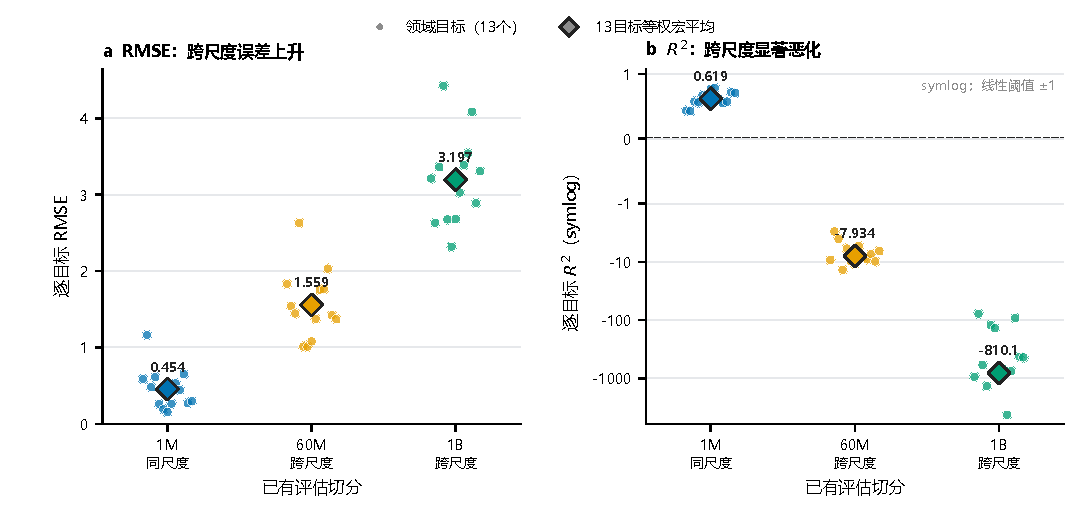
\includegraphics[width=\textwidth]{figures/q2-a-side-cross-scale.pdf}
\caption{A 侧配比模型跨尺度表现}
\label{fig:q2-a-side}
\end{figure}

两条门禁的结论都必须准确表述：这是当前数据条件下的识别性限制，不是 $p$ 或 $Q$
无效的证据。M1 与 M2 的状态记为未估计，而非估计为零。要重开这两道门，需要的
是对 B 侧各训练运行可追溯的配比配置、能够在控制 $N$、$D$ 与模型族之后仍有变异的
多个独立配方，以及独立于配比的质量变化证据，三者缺一不可。本文按题目要求把这些
前置条件作为后续工作的入口列出，而不在缺少证据时给出系数。

\subsubsection{稳健性小结}

除上述验证外，本文另做了两项诊断。其一为删项诊断，用于确认两个规模方向的必要性：
去掉 $N$ 项后 $R^2$ 降至 $0.5352578$、RMSE 升至 $0.2331907$，去掉 $D$ 项后
$R^2$ 降至 $0.4647400$、RMSE 升至 $0.2502578$，二者均说明两个方向不可省略；该
诊断只用于说明模型结构，不参与选型。其二为留一轨迹交叉验证，五折整轨迹分组下
$n=1176$、RMSE $=1.5144\times10^{-4}$、$R^2=0.99999980$，2000 次重抽样的区间为
$[1.2563\times10^{-4},1.7918\times10^{-4}]$。

本问全部区间估计共同受一条限制：独立的轨迹簇只有 8 条。百分位区间对簇数敏感，
因此上文的区间都应读作稳定性提示，而不是高精度总体区间。这一点在解释弹性差异时
尤为重要——$\varepsilon_N$ 与 $\varepsilon_D$ 的逐规模趋势在八条轨迹上单调且一致，
但若要在更细的尺度上作比较，现有簇数不足以支撑。

\subsection{本章小结}

本问的交付如下。经典分支方面，$L=E+AN^{-\alpha}+BD^{-\beta}$ 在 B1 的 1176 个
检查点上拟合得 $E=1.689798$、$A=0.353980$、$\alpha=0.339977$、$B=1.240306$、
$\beta=0.279878$，内样本 $R^2=0.99999982$；缩放雅可比满秩、条件数 $56.378$，
24 组初值全部收敛，留一规模 RMSE 在 $1.02\times10^{-4}$ 至 $2.20\times10^{-4}$ 之间。
弹性方面，中位点处 $\varepsilon_N=-0.048225$、$\varepsilon_D=-0.036924$，
逐规模呈 $\varepsilon_N$ 减弱、$\varepsilon_D$ 增强并约在 1b 附近交叉的格局。
替代条件方面，在半合成网格上，质量评分提高 $0.1$ 约等价于 $0.12$B 参数量
（B6 为 $-0.121915$B、B7 为 $-0.118205$B），该结果只作条件性示例。

本问的结论受三条限制约束。第一，质量方向的系数来自半合成数据，不是实测观测，
B6 与 B7 的样本大量重合、B8 方向相反，故不合并估计单一质量弹性。第二，配比方向的
识别门禁失败，可连接损失的 17 维配比向量为 0，M1 未经估计；这不是配比无效的证据。
第三，B4 与 B5 相对 B1 的损失量尺不可比，可比记录数为 0，因此本问不报告合并的
外部验证指标，只报告分来源误差。

本问交付给问题三的是三个量：经典分支的五个参数与其不确定性、各因素的弹性结构，
以及质量基线 $Q_0=0.498478$。问题三在此基础上构造算力约束下的资源分配模型；
由于 $p$ 与 $Q$ 的独立效应在本问未获识别，问题三的联合优化须在证据支持的变量
范围内进行，其处理方式见下一章。


% ==========================================================
\clearpage
\section{问题三的模型建立与求解}

% ============================================================
% ⚠ 问题三的陷阱（U13--U16）
%   · "罚函数系数取 1 即可保证收敛" ——【无此数学保证】（U13）
%   · 不得把资源配置改成"该加 N 还是加 D"的分类问题（U14）
%   · 不得采用任何预置的最优解数值（U15）
%   · 题目明文要求【讨论成本函数选择对最优解的影响】，
%     附录 B 给了指数型/幂函数型/对数渐进型三型 —— 必须做（U16）
% ============================================================


\subsection{问题三分析}

本问在总算力预算 $C$ 受限的条件下，在参数量 $N$、数据量 $D$、领域配比 $p$ 与数据
质量 $Q$ 之间分配资源，并分析预算跨越不同量级时最优分配是否发生本质改变。算力消耗
由三部分组成：基础训练开销 $C_{\mathrm{train}}=6ND$、数据质量提升开销
$C_Q=D[g(Q)-g(Q_0)]_+$ 与长文本注意力开销 $C_{\mathrm{attn}}=\eta ND L_{\mathrm{ctx}}$，
其中 $\eta=2\times10^{-4}$。上下文长度 $L_{\mathrm{ctx}}$ 由模型架构与任务需求外生
给定，其可行取值须依据附件 C7，本题不把它作为内点寻优变量，但要求解析给出使注意力
开销与训练开销相当的临界长度，并在其可行取值上完成敏感性分析。题目建议考察
$10^{19}$、$10^{22}$、$10^{24}$ FLOPs 三档预算，并至少覆盖三个不同量级。

本问的困难有三处。第一，质量成本函数的量纲与量级需要先固定下来，否则约束的可行性
判断无从谈起：三种候选 $g(Q)$ 在同一 $Q$ 上的取值可相差一个量级以上，这会直接改变
哪些 $Q$ 是负担得起的。第二，按问题二的审计结论，配比的独立效应与质量的独立效应
在当前数据下均未获识别，因此把 $p$ 或 $Q$ 当作由数据驱动的内点决策变量是没有依据
的；本问必须在"哪些量可以寻优、哪些量只能固定"这一点上给出明确交代，而不是先在
形式上写一个四变量优化、再悄悄把两个变量固定。第三，题目要求判断"结构性转移"，
这需要一个可证伪的定义：若只凭图形观察就宣称策略发生了质变，结论无法复核。

\subsection{模型建立}

\subsubsection{优化模型与变量域}

记决策向量为 $(N,D,Q,p)$，目标为最小化问题二冻结模型给出的预测损失：

\begin{equation}
\min_{N,D,Q,p}\ \hat L_{M0}(N,D)
\quad\text{s.t.}\quad
C_{\mathrm{train}}+C_Q+C_{\mathrm{attn}}\le C
\end{equation}

式中各项为

\begin{equation}
C_{\mathrm{train}}=6ND,\qquad
C_Q=D\bigl[g(Q)-g(Q_0)\bigr]_+,\qquad
C_{\mathrm{attn}}=\eta\,N\,D\,L_{\mathrm{ctx}}
\end{equation}

其中 $[\cdot]_+=\max(\cdot,0)$，$Q_0$ 为问题一交付的质量基线。可行性区域为
$N>0$、$D>0$、$Q_0\le Q\le 1$、$p_i\ge0$ 且 $\sum_i p_i=1$。质量一侧只允许
提升而不允许下降，这一限制来自 $[\cdot]_+$ 的增量成本约定：若不设下界，优化器会把
低于基线的质量当作零成本选项，从而给出一个以降低质量为代价换取更多参数的解，这在
题意上不成立。

变量 $p$ 的处理需要一个明确交代。题目允许把 $p$ 作为联立决策变量，也可以由前两问
结果确定，但须说明理由。本文不把 $p$ 作为决策变量，理由是问题二的识别性审计：
附件 B 中可逐行连接到损失的 17 维配比向量为 0 个，$p$ 对损失的经验响应面不存在，
模型 $M0$ 本身也不含 $p$ 项。在这样的证据条件下把 $p$ 写进决策向量，等价于对
$\partial L/\partial p$ 赋予一个未经估计的数值，得出的"最优配比"只是该假设的算术
推论，不具备可验证性。因此本文在固定 $Q=Q_0$、不含 $p$ 的受限模型上求解，并把这一
范围的边界在结果中显式标出。

\subsubsection{质量成本函数与临界上下文长度}

题目附录 B 给出三种 $g(Q)$ 及其参数，本文原样采用：

\begin{equation}
g_{\exp}(Q)=\gamma e^{\lambda Q},\quad
g_{\mathrm{pow}}(Q)=\gamma Q^{\lambda},\quad
g_{\log}(Q)=\gamma\ln(1+\lambda Q)
\end{equation}

式中，指数型的 $\gamma=10^{7}$、$\lambda=6.0$；幂函数型的 $\gamma=5\times10^{9}$、
$\lambda=4.0$；对数渐进型的 $\gamma=2\times10^{9}$、$\lambda=10.0$。三种形式的
形状差异决定了质量成本随 $Q$ 上升的快慢，是题目要求比较的对象。

临界上下文长度可由两项开销之比直接解出。记 $C_{\mathrm{attn}}/C_{\mathrm{train}}
=\eta L_{\mathrm{ctx}}/6$，令其等于 1，得

\begin{equation}
L_{\mathrm{ctx}}^{\mathrm{crit}}=\frac{6}{\eta}=\frac{6}{2\times10^{-4}}=30000
\end{equation}

式中，$L_{\mathrm{ctx}}^{\mathrm{crit}}$ 为注意力开销与训练开销相等的上下文长度。
当 $L_{\mathrm{ctx}}<30000$ 时训练开销占优，大于该值时注意力开销占优，且比值
等于 $L_{\mathrm{ctx}}/30000$。该结果是题面成本公式的代数推论，不依赖任何拟合
参数，也不依赖 $Q$ 的取值，因而可作为纯解析结论使用。

\subsubsection{结构性转移的定义与识别方法}

题目要求给出结构性转移的"明确数学定义与识别方法"。本文把转移定义在相邻情景对
之间：相邻指预算取相邻档位而上下文长度固定，或上下文长度取相邻档位而预算固定。
对每一对情景，记录其活动约束集合与成本份额向量

\begin{equation}
s=\bigl(s_{\mathrm{train}},s_Q,s_{\mathrm{attn}}\bigr),\qquad
s_j=\frac{C_j}{C_{\mathrm{train}}+C_Q+C_{\mathrm{attn}}}
\end{equation}

并定义份额转移量

\begin{equation}
T=\tfrac12\sum_{j}\bigl|s_j^{(b)}-s_j^{(a)}\bigr|
\end{equation}

式中，$T$ 为两个情景之间成本份额向量的总变差距离，取值于 $[0,1]$。判定规则为：
把问题二的参数不确定性按整轨迹 bootstrap 传播到两情景的选择上，若活动约束集合的
改变在 bootstrap 中的发生概率不低于 $0.95$，或 $T$ 的第 5 百分位超过数值误差带
$\epsilon_{\mathrm{num}}$，则判该对情景之间存在结构性转移。$\epsilon_{\mathrm{num}}$
定义为同一情景下按常规与更严格两种求解容差各算一次所得的 $T$ 的最大值，两组容差
须在运行前登记，使判据不受事后调参影响。各 $(Q_0,g)$ 组合分别判定，全部组合一致
才算"稳健转移"，否则记为"条件性转移"。这条规则的意义在于把"质的变化"从图形判断
变为可复核的统计判据；在参数 bootstrap 缺失时，规则明确要求只报告描述性变化而不
作转移判定。

\subsection{模型求解}

求解在冻结的 B1 实测网格上进行，不做连续松弛：候选点为问题二审计确认的 1176 个
$(N,D)$ 组合，即 8 个参数规模与 147 个训练检查点的全部组合。选择离散网格而非连续
变量，是为了避免求解结果越出 B1 的支持范围——若允许 $N$、$D$ 连续取值，模型会外推到
未观测区域，而问题二已经表明该模型不具备跨尺度外推能力。计算全部使用精确有理数
运算，先把以十亿为单位的 $N_B$、$D_B$ 还原为整数绝对量，再计算三项开销，避免浮点
误差在 $(10^{24})$ 量级上的累积。平局时按预测损失、总成本、参数量、数据量、记录
编号依次排序，使选择唯一确定。

上下文长度取 C7 中实际出现的五个离散值，即 2048、4096、8192、32768 与 131072，
与三档预算交叉得到 15 个情景。为评估选择对参数不确定性的敏感性，把问题二保存的
1000 组整轨迹 bootstrap 参数逐一代入，在每个情景下重新筛选可行点并重新选择最优，
记录选择频率与预测损失的百分位区间。

质量一侧的求解分两支。主支固定 $Q=Q_0$，此时 $[g(Q_0)-g(Q_0)]_+=0$，故 $C_Q\equiv0$，
预算全部由训练与注意力两部分消耗。由于 $Q$ 不影响损失也不产生成本，三种 $g(Q)$
在本支中不参与选择——这是一个必须说明的结果，而不是遗漏。作为独立的一支，本文另
计算从 $Q_0$ 到 $Q=1$ 的纯质量成本曲线，用于回答"把质量提升到某个水平需要多少
算力"。

第三支是条件性的质量—损失响应模型。记质量响应系数为 $\beta_Q$，

\begin{equation}
L_{\mathrm{cond}}(N,D,Q\mid\beta_Q)=\hat L_{M0}(N,D)-\beta_Q\,(Q-Q_0),\qquad \beta_Q\ge0
\end{equation}

式中，$\beta_Q$ 为质量每提升一个单位所对应的损失下降。问题二未识别出该系数，故
本文不为它赋任何估计值，而是把它作为自由参数扫描：对每个情景，在剩余预算内把 $Q$
提升到可负担的最大值，得到不同 $N$、$D$ 组合关于 $\beta_Q$ 的下包络，再报告包络
发生切换的 $\beta_Q$ 取值，即首次发生 $N$ 或 $D$ 重分配的阈值。这一支回答的是
"若质量响应达到多大，资源配置才应当改变"，属于条件性结论。

\subsection{结果分析}

\subsubsection{上下文长度的可行取值}

C7 的审计覆盖 45 个模型架构记录，45 条记录的名称唯一、上下文取值均为正整数且无
缺失，共得到 5 个离散长度，分布见表 \ref{tab:q3-c7}。

\begin{table}[htp!]
\centering
\renewcommand\arraystretch{1.2}
\caption{附件 C7 的上下文长度分布及其相对临界长度的位置}\label{tab:q3-c7}
\begin{tabular*}{\textwidth}{@{\extracolsep{\fill}}lccc@{}}
\toprule
最大位置嵌入数 & 模型数 & 注意力/训练开销比 & 相对临界长度 \\
\midrule
2048   & 18 & 0.0683 & 低于 \\
4096   & 8  & 0.1365 & 低于 \\
8192   & 7  & 0.2731 & 低于 \\
32768  & 11 & 1.0923 & 高于 \\
131072 & 1  & 4.3691 & 高于 \\
\bottomrule
\end{tabular*}
\end{table}

45 个模型中有 12 个（$26.7\%$）的架构上限超过临界长度 30000，33 个不超过。这一
分布说明长上下文在大模型架构中已是常见配置，但并非主流：超过临界值的模型占比约
四分之一，其中最长的 131072 使注意力开销达到训练开销的 $4.37$ 倍。需要说明的是，
C7 记录的是 \texttt{max\_position\_embeddings}，即架构支持的上下文上限，不保证等于实际
部署时使用的窗口；本文按题面要求以该字段确定可行取值集合，其与实际任务窗口的
一致性需由题目设定支持。该分布见图 \ref{fig:q3-c7}。

\begin{figure}[htp!]
\centering

\includegraphics[width=.86\textwidth]{figures/q3-c7-lengths.pdf}
\caption{C7 上下文长度与临界值}
\label{fig:q3-c7}
\end{figure}

\subsubsection{预算与上下文交叉下的参考配置}

固定 $Q=Q_0$ 时 $C_Q=0$，约束退化为 $ND(6+\eta L_{\mathrm{ctx}})\le C$，即在给定
上下文长度下，可负担的"参数量×数据量"上限被一个常数因子压缩。15 个情景全部存在
可行点，最优选择与成本分解见表 \ref{tab:q3-frontier}。

\begin{table}[htp!]
\centering
\renewcommand\arraystretch{1.2}
\caption{15 个预算×上下文情景的参考配置与成本分解}\label{tab:q3-frontier}
\begin{tabular*}{\textwidth}{@{\extracolsep{\fill}}llcccccc@{}}
\toprule
预算 & $L_{\mathrm{ctx}}$ & 选中 $N$ & 选中 $D$ & 预测损失 & 可行点数 & 预算利用率 \\
\midrule
$10^{19}$ & 2048   & 0.162405 & 8.389   & 3.030398 & 39   & 87.325\% \\
$10^{19}$ & 4096   & 0.162405 & 8.389   & 3.030398 & 36   & 92.906\% \\
$10^{19}$ & 8192   & 0.162405 & 6.291   & 3.087766 & 34   & 78.041\% \\
$10^{19}$ & 32768  & 0.162405 & 4.194   & 3.176846 & 27   & 85.506\% \\
$10^{19}$ & 131072 & 0.070542 & 4.194   & 3.392088 & 16   & 95.307\% \\
$10^{22}$ & 2048   & 6.861040 & 226.492 & 2.145611 & 1060 & 99.603\% \\
$10^{22}$ & 4096   & 6.861040 & 211.812 & 2.150759 & 1049 & 99.100\% \\
$10^{22}$ & 8192   & 6.861040 & 188.744 & 2.159845 & 1032 & 98.916\% \\
$10^{22}$ & 32768  & 2.782831 & 285.213 & 2.194660 & 969  & 99.638\% \\
$10^{22}$ & 131072 & 2.782831 & 111.149 & 2.271591 & 793  & 99.642\% \\
$10^{24}$ & 2048   & 11.965825 & 299.893 & 2.093379 & 1176 & 2.300\% \\
$10^{24}$ & 4096   & 11.965825 & 299.893 & 2.093379 & 1176 & 2.447\% \\
$10^{24}$ & 8192   & 11.965825 & 299.893 & 2.093379 & 1176 & 2.741\% \\
$10^{24}$ & 32768  & 11.965825 & 299.893 & 2.093379 & 1176 & 4.505\% \\
$10^{24}$ & 131072 & 11.965825 & 299.893 & 2.093379 & 1176 & 11.560\% \\
\bottomrule
\end{tabular*}
\end{table}

（表中 $N$ 的单位为十亿参数，$D$ 的单位为十亿 token。）

三个预算档给出三种性质不同的结果。$10^{22}$ 档的预算被用尽，利用率在
$98.92\%$--$99.64\%$ 之间，说明该档下约束是紧的，选择由预算边界决定；选中点落在
$N$ 与 $D$ 的中段，随上下文长度增加而减少数据量以腾出注意力开销。$10^{19}$ 档
从未用尽预算（$78.04\%$--$95.31\%$），原因是可行网格在该量级上已经稀疏，可用
点上界不足以触及预算边界。$10^{24}$ 档则出现明显的支持域受限：1176 个网格点
全部可行，最优解一律落在网格上界 $N=11.965825$B、$D=299.893$B，五个上下文的预测
损失与训练开销完全相同，利用率仅 $2.300\%$--$11.560\%$，档内差异全部来自注意力
开销。

最后一档的结论必须谨慎表述。利用率低并不意味着"预算没有被有效利用"，而是意味着
B1 网格的最大规模已经无法消耗掉这一量级的预算；在网格之外的更大 $N$、$D$ 上损失
是否继续下降，本模型没有数据支持回答。因此该档结果只能读作"在 B1 支持范围内，
$10^{24}$ 档的约束不起作用"，不能外推为更大规模的结论。15 个情景的利用率分布见
图 \ref{fig:q3-frontier}。

\begin{figure}[htp!]
\centering
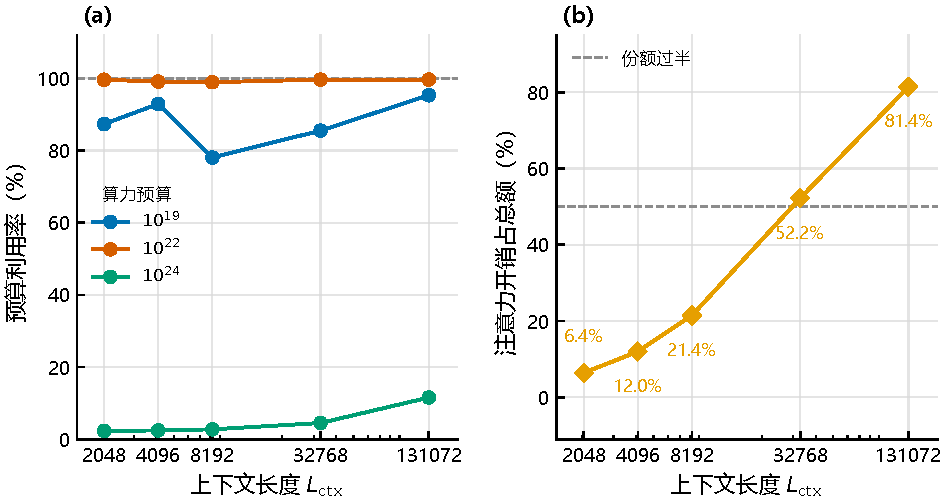
\includegraphics[width=.92\textwidth]{figures/q3-frontier.pdf}
\caption{预算情景利用率与成本份额}
\label{fig:q3-frontier}
\end{figure}

\subsubsection{成本结构只由上下文长度决定}

在 $C_Q=0$ 的设定下，成本份额有一个简洁的解析形式。由
$C_{\mathrm{attn}}/C_{\mathrm{train}}=L_{\mathrm{ctx}}/30000$ 可得

\begin{equation}
s_{\mathrm{attn}}=\frac{L_{\mathrm{ctx}}/30000}{1+L_{\mathrm{ctx}}/30000},\qquad
s_{\mathrm{train}}=1-s_{\mathrm{attn}}
\end{equation}

该式表明份额与预算和选中点都无关，只随上下文长度变化。代入五个可行长度得
表 \ref{tab:q3-share}。

\begin{table}[htp!]
\centering
\renewcommand\arraystretch{1.2}
\caption{成本份额随上下文长度的变化（与预算档位无关）}\label{tab:q3-share}
\begin{tabular*}{\textwidth}{@{\extracolsep{\fill}}lccccc@{}}
\toprule
$L_{\mathrm{ctx}}$ & 2048 & 4096 & 8192 & 32768 & 131072 \\
\midrule
训练开销份额 & 93.610\% & 87.987\% & 78.550\% & 47.795\% & 18.625\% \\
注意力开销份额 & 6.390\% & 12.013\% & 21.450\% & 52.205\% & 81.375\% \\
\bottomrule
\end{tabular*}
\end{table}

这一结构给出一个直接的工程判读：当上下文长度取 32768 时，超过一半的算力预算被
注意力开销吃掉；取 131072 时，训练本身只占约 $18.6\%$ 的预算。换言之，长上下文的
代价不是边际性的，而是会改变预算的主要去向。这正是题目要求考察 $L_{\mathrm{ctx}}$
对最优配置影响的实质。图 \ref{fig:q3-dashboard} 把配置、成本构成与预测损失放在
一起对照：面板 (a)(b) 给出各情景选中的 $N$ 与 $D$，空心圈标出触及 B1 支持上界
的点；面板 (c) 是三类成本的百分百堆叠，直观显示注意力份额如何随上下文长度吞掉
训练份额；面板 (d) 为对应的 M0 预测损失。四张面板合读可以看到一件事：$10^{24}$
档的五条线全部终止在支持上界，其损失也全部停在同一点，说明该档的差异已不由预算
决定，而由可用网格决定。图中的 22 对相邻情景仅作描述性比较；本图不使用 bootstrap
或 KKT 判据，不能据此宣称发生结构性转移。

\begin{figure}[htp!]
\centering
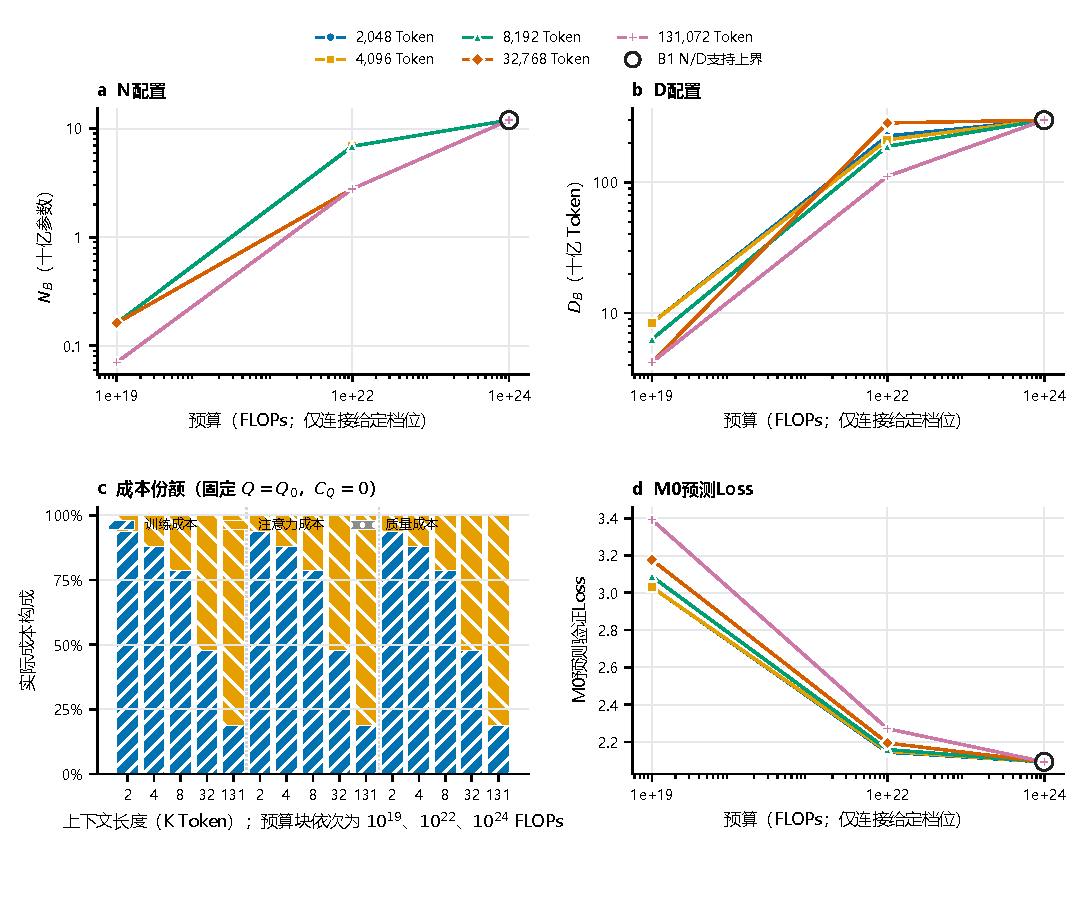
\includegraphics[width=\textwidth]{figures/q3-resource-dashboard.pdf}
\caption{资源配置与成本分解}
\label{fig:q3-dashboard}
\end{figure}

\subsubsection{成本函数选择的影响}

三种 $g(Q)$ 的影响需要分两个层次回答。在固定 $Q=Q_0$ 的主支中，$C_Q\equiv0$，
三种形式对最优选择没有任何影响——这一点在结果中直接可见：表 \ref{tab:q3-frontier}
的每一行都与 $g$ 的选取无关。但这不等于成本函数的选择不重要，而是说明在"不提升
质量"的策略下质量成本不进入约束。

在质量提升支中，三种形式的差异显著。把质量由 $Q_0$ 提升到 $Q=1$，在 B1 数据量的
中位值（$D=146.801$B token）处，三种形式所需的增量算力分别为

\begin{table}[htp!]
\centering
\renewcommand\arraystretch{1.2}
\caption{质量提升的增量算力}\label{tab:q3-cq}
\begin{tabular*}{\textwidth}{@{\extracolsep{\fill}}lccc@{}}
\toprule
成本函数 & $g(Q_0)$ & $g(1)-g(Q_0)$ & 增量算力 $C_Q$ \\
\midrule
指数型     & $1.9903\times10^{8}$ & $3.8353\times10^{9}$ & $5.6302\times10^{20}$ \\
幂函数型   & $3.0871\times10^{8}$ & $4.6913\times10^{9}$ & $6.8869\times10^{20}$ \\
对数渐进型 & $3.5784\times10^{9}$ & $1.2174\times10^{9}$ & $1.7871\times10^{20}$ \\
\bottomrule
\end{tabular*}
\end{table}

式中各量的单位均为 FLOPs（$g$ 为每 token 成本，乘以 $D$ 后为总量）。三种形式的
增量算力相差约 $3.9$ 倍，对数渐进型最省、幂函数型最贵。由于增量算力与数据量成正比，
其可负担性同时取决于 $D$ 的取值。在 B1 支持上界（$D=299.893$B）处，把质量提升到
1 所需的算力约为 $10^{21}$ 量级，相当于 $10^{22}$ 档预算的 $11.5\%$、$14.1\%$ 与
$3.7\%$，而在 $10^{19}$ 档下远超预算。反过来，若要在 $10^{19}$ 档内完成这一提升，
数据量必须压到 $2.607$B（指数型）、$2.132$B（幂函数型）或 $8.215$B（对数渐进型）
以下。把该界与表 \ref{tab:q3-frontier} 的参考配置对照可以看出：$10^{19}$ 档选中的
$D$ 为 $4.194$B 至 $8.389$B，因此指数型与幂函数型在该档的参考配置上完全不可行，
对数渐进型只在 8192 及以上三个上下文处可行、在 2048 与 4096 处仍不可行。这说明
"成本函数的选择影响最优解"在本问是实质性的：换一种 $g(Q)$，最低预算档下质量提升
从"完全不可能"变为"部分可行"。质量成本曲线见图 \ref{fig:q3-cost}，其中横轴为
质量水平、纵轴为对数刻度的增量算力，三条预算参考线标出了各档的可负担边界。

\begin{figure}[htp!]
\centering
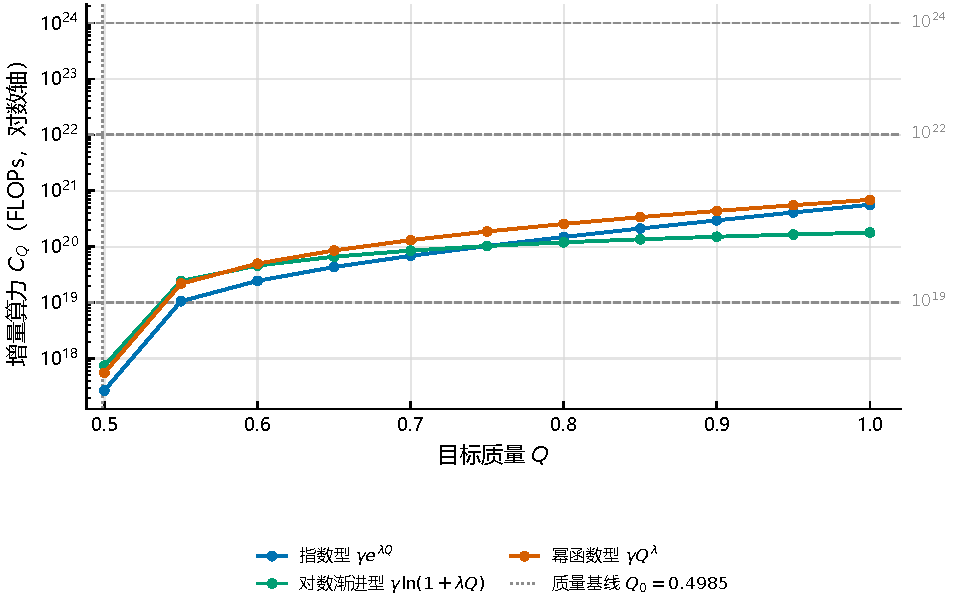
\includegraphics[width=.92\textwidth]{figures/q3-cost-curve.pdf}
\caption{质量成本函数比较}
\label{fig:q3-cost}
\end{figure}

\subsubsection{相邻情景的比较与条件性重分配}

22 对相邻情景中，17 对的最优配置发生了变化，5 对保持不变——后者包括 $10^{19}$ 档
的 2048 到 4096 一步，以及 $10^{24}$ 档因触及网格上界而配置固定的四对。份额转移量
$T$ 在固定上下文的预算对上恒为 $0$，这与前一小节的解析结论一致：成本份额只依赖
$L_{\mathrm{ctx}}$，预算变化只改变可行点数量而不改变份额结构。固定预算、改变上下文
的对则给出非零的 $T$，最大值出现在 8192 到 32768 一步（$T=0.3076$），对应注意力
份额从 $21.45\%$ 升到 $52.21\%$ 的跃变。

条件性质量响应模型的结果如下。45 个情景（3 档预算 × 5 个上下文长度 × 3 种成本
函数）的下包络共切分为 166 段；其中 15 个情景（全部位于 $10^{24}$ 档）不存在
$N$、$D$ 的重分配，因为在网格上界处任何质量响应都不会改变选择；其余 30 个情景
存在有限的重分配阈值，取值落在 $0.003241$ 至 $0.624520$ 之间。阈值较小的情景
（如 $10^{22}$ 档配合对数渐进型，阈值约 $0.0032$）意味着质量响应稍大于零就足以
改变最优配置；阈值较大的情景（如 $10^{19}$ 档配合指数型，阈值约 $0.6245$）则
需要相当强的质量响应才会触发重分配。这一谱系本身就是"成本函数选择影响最优解"
的定量体现：同一预算下，换个 $g(Q)$ 会使重分配阈值移动一至两个数量级。三个预算档
与三种成本函数下的阈值分布见图 \ref{fig:q3-cond}。

\begin{figure}[htp!]
\centering

\includegraphics[width=.96\textwidth]{figures/q3-conditional.pdf}
\caption{质量响应阈值}
\label{fig:q3-cond}
\end{figure}

需要重申该支的性质：$\beta_Q$ 未经数据识别，因此上述阈值不是"实测最优质量"，而是
形如"若响应系数达到某值，配置在何处改变"的条件性结论。本文不为 $\beta_Q$ 编造
估计值，也不把它当作问题二的输出。

\subsection{模型验证与灵敏度分析}

参数不确定性的传播结果是本节的主要验证内容。把问题二保存的 1000 组整轨迹
bootstrap 参数逐一代入，在 15 个情景中重新筛选可行点并重新选择：15 个情景下
原选中点均在 1000/1000 次重抽样中被重新选中，选择频率为 $1.0$，场景内不出现
第二个被选中的网格点。预测损失的百分位区间很窄，最宽的一处（$10^{19}$ 档配合
2048）也只有 $1.3\times10^{-4}$。这一结果说明：在既定的 M0 函数形式与 B1 支持
网格内，参考配置对参数重抽样是稳定的。

但稳定性的范围必须划清。该检验只覆盖参数不确定性，不覆盖三类误差：M0 的函数形式
误设、B1 与目标训练方案之间的迁移误差，以及网格之外的行为。此外，$10^{24}$ 档的
选择受网格上界约束，较窄的 bootstrap 区间不能解除这一边界。因此上述结果支持的是
"在当前模型与数据范围内选择稳定"，不支持"该配置就是全局最优"。逐情景的区间与
配置切换概率见图 \ref{fig:q3-bootstrap}：面板 (a)(b) 中 $N$ 与 $D$ 的区间在全部
15 个情景中退化为单点（图中未作放大），面板 (c) 给出预测损失的 $2.5\%$–$97.5\%$
区间，面板 (d) 的配置切换概率在每个情景上都是 $0\%$，即原配置在 1000 次重抽样中
从未被替换。面板 (d) 的观感是一条贴在零刻度上的竖线，这本身就是结论——切换从未
发生，而不是没有数据。

\begin{figure}[htp!]
\centering
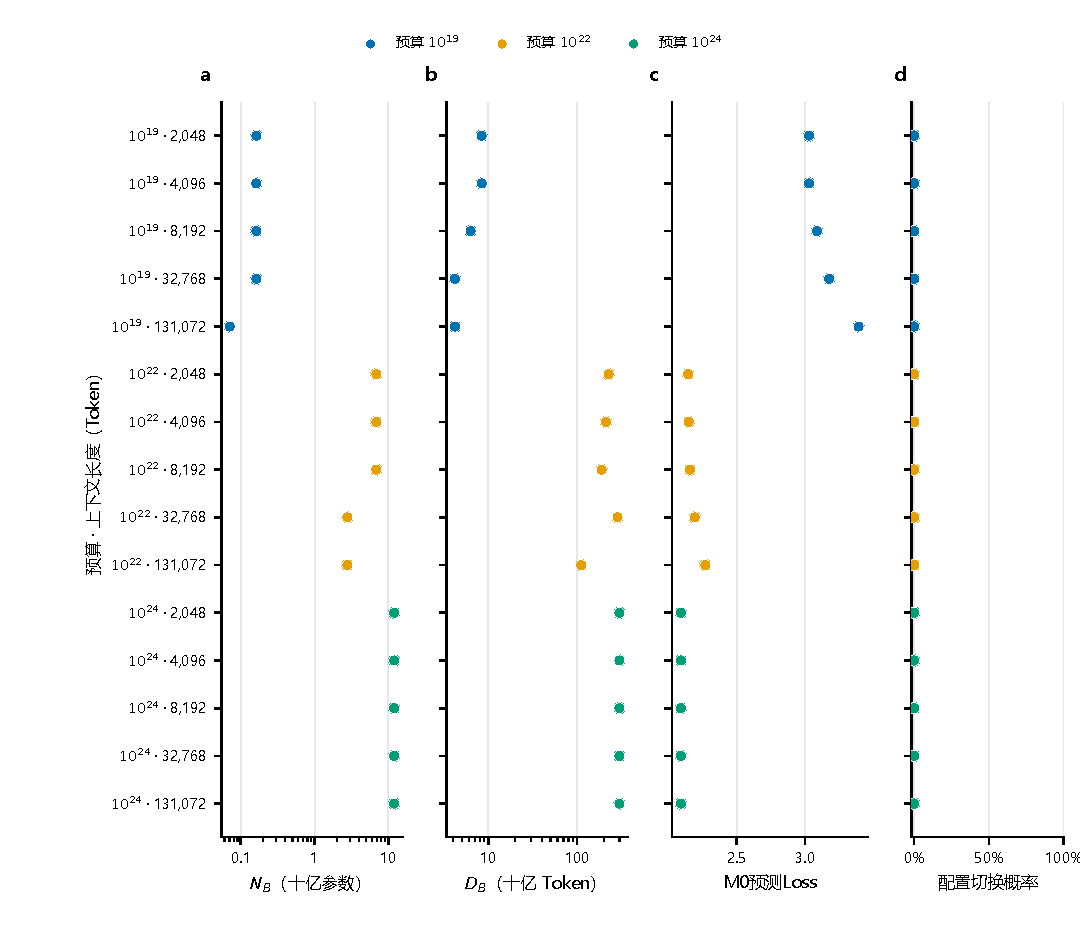
\includegraphics[width=\textwidth]{figures/q3-bootstrap-stability.pdf}
\caption{配置选择的重抽样稳定性}
\label{fig:q3-bootstrap}
\end{figure}

求解的数值可靠性另有两项证据。其一，全部开销计算使用精确有理数运算而非浮点，
可排除 $10^{24}$ 量级上的舍入累积；其二，约束的可行性判定在每个情景中都与独立
重算的可行点计数核对一致（表 \ref{tab:q3-frontier} 的"可行点数"一列）。C7 的输入
以 SHA-256 与脚本哈希一并登记，可复算。

质量基线的选择本身也是一项需要检验的设定：问题一给出两个候选，本文取
$Q_{\mathrm{huber}}=0.498478$ 为主分、$Q_{\mathrm{eq}}=0.496223$ 为敏感性对照。
把两者分别代入同一套预算、上下文、B1 网格与 M0 后重解，图 \ref{fig:q3-qbase}
显示两条分支给出的 $N$、$D$ 与预测损失在每个情景上完全重合，逐情景的最大绝对差
为 $0$。该图是一张零结果图，它的价值在于排除一种可能的质疑——即问题三的结论是否
依赖问题一那个在两候选间无法用证据区分的操作性选择。答案是：不依赖。需要说明的
是，两支都固定在各自基线、$C_Q$ 均为零，因此这一对照只说明"主分口径不影响预算
分配"，不构成质量收益的实证估计，也不构成配比与质量的联合优化。

\begin{figure}[htp!]
\centering
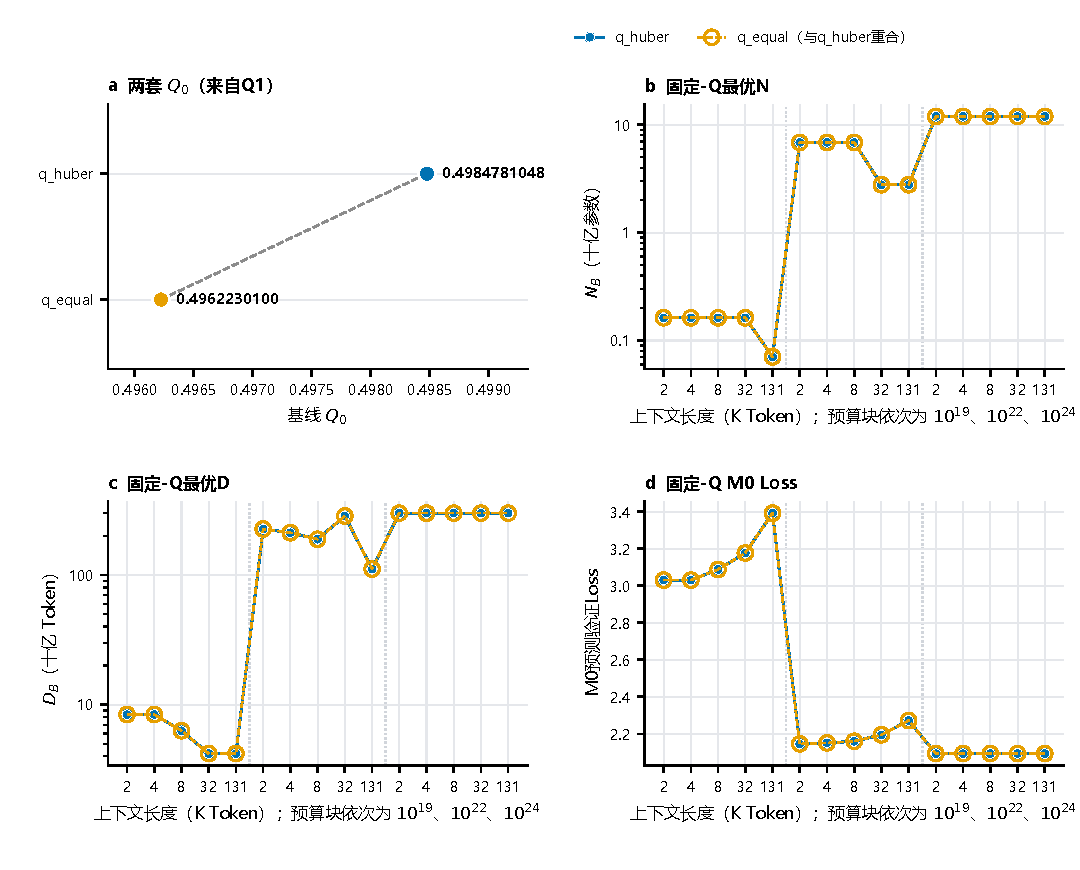
\includegraphics[width=\textwidth]{figures/q3-q-baseline-sensitivity.pdf}
\caption{质量基线的配置敏感性}
\label{fig:q3-qbase}
\end{figure}

本节必须明确写出尚未执行的部分。按 \ref{sec:q2-sens} 设定的结构性转移判据，
正式的转移判定需要活动约束集合在 bootstrap 下的改变概率与份额转移量的第 5 百分位，
而本文的 bootstrap 只传播了问题二的参数不确定性，且质量成本份额在 $Q=Q_0$ 时恒为
零，因此活动约束集合在情景之间不存在统计意义上的可变性。本文据此不作出结构性
转移的判定，只报告上文描述性的配置与份额变化。若要完成正式判定，需要先在问题二
的配比与质量响应上取得可识别的证据，使 $p$ 或 $Q$ 能够真正进入约束并产生可变的
活动集合。

其余限制一并列出。第一，$p$ 未作为决策变量，本问不回答领域配比的优化问题，理由
是问题二的 $p$ 门禁失败。第二，$Q$ 在主支中固定于基线，因此本问给出的是
"在现有质量水平下如何分配算力"，而非"应当把质量提升到多少"。第三，$N$、$D$ 只在
B1 的 $8\times147$ 实测网格上搜索，不插值不外推，$10^{24}$ 档的结果因此受网格
上界限制。第四，正式的质量—损失响应面仍需问题二提供可识别的独立质量变化证据。

\subsection{本章小结}

本问的交付如下。约束结构方面，三部分开销按题面公式设定，解析给出使注意力开销与
训练开销相等的临界上下文长度 $L_{\mathrm{ctx}}^{\mathrm{crit}}=6/\eta=30000$，
并据此确认 C7 的 45 个架构记录中有 12 个（$26.7\%$）超过该临界值。参考配置方面，
固定质量基线后 $C_Q\equiv0$，15 个预算×上下文情景全部可行；$10^{22}$ 档预算用尽
（利用率 $98.92\%$--$99.64\%$），$10^{19}$ 档未触及边界
（$78.04\%$--$95.31\%$），$10^{24}$ 档的 1176 个网格点全部可行、最优解落在网格
上界而利用率仅 $2.300\%$--$11.560\%$。成本结构方面，注意力开销份额只由上下文
长度决定，从 2048 处的 $6.390\%$ 升至 131072 处的 $81.375\%$。成本函数选择方面，
三种 $g(Q)$ 在固定质量的主支中不影响选择；在质量提升支中，把质量由 $Q_0$ 提升到
1 所需算力相差约 $3.9$ 倍（对数渐进型最省），且该开销与 $D$ 成正比，故在
$10^{19}$ 档的参考配置上指数型与幂函数型完全不可行、对数渐进型仅部分可行。

本问的结论受三条限制约束。第一，未作结构性转移判定：判据已按可证伪的要求
预先定义，但正式判定所需的活动约束可变性依赖问题二尚未识别的配比与质量响应，故本章
只报告描述性的份额与配置变化。第二，$p$ 未作为决策变量，$Q$ 在主支中固定于基线，
因此本问回答的是给定质量水平下的算力分配，不是 $N$、$D$、$p$、$Q$ 的联合最优。
第三，候选点限于 B1 实测网格，$10^{24}$ 档的结果受网格上界限制，不能外推为更大
规模的结论。

本问交付给问题四的是算力约束下的配置关系与成本结构：问题四在把损失翻译为能力得分
时，可以据此说明算力增长放缓情景下的配置含义。


% ==========================================================
\clearpage
\section{问题四的模型建立与求解}

% ============================================================
% ⚠ 问题四的陷阱（U17--U20）
%   · 【必须分解并量化规模扩张与非规模技术进步各自的贡献占比】——
%     这是本问的核心必答任务，U18 明确诱导你"无需分解"（U18）
%   · Benchmark 不得按 10 分分档改成分类预测，必须做连续前沿预测（U17）
%   · 不得采用任何预置的分解系数（U19）
%   · Loss–Benchmark 相关系数的【符号与方向必须独立检验】（U20）
%   另：题目要求对 C8 做【至少一项逐任务聚合分析】，不得只用汇总表。
% ============================================================

% ★ 已锁定 F 题：共 4 问，本章保留

\subsection{问题四分析}

\subsection{模型建立}

\subsection{模型求解}

\subsection{结果分析}

\subsection{模型验证与灵敏度分析}

\subsection{本章小结}


% ==========================================================
\clearpage
\section{模型稳健性与综合检验}\label{sec:q3-sens}

% ============================================================
% ★★ 本章是【刻意加出来的加分章】★★
%
%   经逐篇核对 5 篇往届优秀论文（B题76页 / C题78页 / E题93页 / E题69页
%   / F题116页）：【没有一篇做了消融实验、超参数灵敏度扫描或误差分解】。
%   这是明确的空白区——谁做谁超基准线，而且是"中期做、后期写"的活，
%   不占用建模主线的关键路径。
%
%   本章只放【跨问共用】的内容，与该问专属的 x.5 节不重复。
% ============================================================

\subsection{参数灵敏度与随机性}

本章只汇总跨问共用的稳健性证据，各问专属的灵敏度分析仍见其 x.5 节，不在此重复。
汇总的目的是回答一个问题：本文三项交付的结论，在多大的参数与随机性扰动下仍然成立。

第一项是质量评分对字段设定与权重构造的敏感性。剔除 7 个语义未追溯字段后，A1 样本分
的 P95 绝对差为 $0.113048$、最大差 $0.255681$，A2 上的秩相关降至 $0.729556$；这是
全部敏感性场景中影响最大的一处。Huber 阈值折半只带来 $0.007374$ 的宏平均位移
（秩相关 $0.980$），权重指数 $\alpha$ 取 $0.5$ 与取 $1$ 给出完全相同的样本分。把
两个质量候选分别代入问题三重解，$N$、$D$ 与预测损失在 15 个情景上的最大绝对差均为
$0$——即预算分配的结论不依赖问题一那个在证据上无法区分的选择。

第二项是评分与资源配置对随机抽样的敏感性。评分的域级聚合使用 $B_Q=2000$ 次记录级
bootstrap 的百分位区间；问题二的标度律参数使用 1000 次整轨迹整簇 bootstrap，留一
规模检验的留出 RMSE 落在 $1.02\times10^{-4}$ 至 $2.20\times10^{-4}$ 之间；问题三把
这 1000 组参数逐一传播到 15 个情景，原选中点在全部重抽样中保持不变，选择频率为
$1.0$。三处随机化给出的结论一致：在既定的模型形式与数据支持范围内，本文的选择对
重抽样是稳定的。

但"稳定"的边界必须同时说明，否则容易被读成超出证据的强结论。问题二与问题三的
bootstrap 都只基于 8 条 B1 轨迹，区间因此很窄，而窄的原因是独立簇只有 8 个，
不是参数精度高；$10^{24}$ 档的选择受 B1 网格上界约束，更窄的区间并不能解除这一
边界。质量评分的敏感性分析同样只覆盖预处理与权重设定，不覆盖原始语料的生成过程。

\subsection{消融实验}

本稿未完成逐模块移除、重拟合并在统一留出集上比较的完整消融实验。Q1.3 的配比与
派生质量特征对照只检验一个受限扩展，且不能识别独立质量效应；二次面结果属于结构敏感性
分析。二者均不替代完整消融，因此本章不报告各模块的消融贡献。

\subsection{误差分解与失效案例}

本稿未完成按数据来源、模型形式与观测层级划分的定量误差分解，因此不报告误差贡献占比。
现有失效证据可作为边界而非误差分摊：A 侧配比模型跨至 60M 与 1B 时 $R^2$ 分别为
$-7.9336$ 与 $-810.12$；B4/B5 与 B1 的损失协议不可比；B1 bootstrap 只有 8 条独立轨迹。
这些结果说明迁移、量尺与簇数限制，但不能据此推算各误差来源所占比例。

\subsection{外推与分布偏移}

三项交付在外推方向上的表现并不一致，这本身是一个需要分别报告的结论。

配比—损失模型不具备跨尺度定量外推能力。同尺度检验集 A6/A7 上 $R^2=0.6189$、
Spearman $=0.8327$；换到 60M 与 1B 的跨尺度切分后，$R^2$ 分别降到 $-7.9336$ 与
$-810.12$，而秩相关仍保持 $0.73$--$0.83$。同时失去量级校准、保住排序，说明该模型
在训练尺度之外可用的是配比的相对优劣，而不是损失的绝对水平。

A12 至 A15 的估计表不构成独立留出验证。这四张表的数据角色是外推估计而非实测，
本文只用它们做一致性核对，不据此宣称外推能力；\ref{sec:q1-mixres} 已说明其口径。

标度律的外推边界由支持域决定。B1 的参数量覆盖 $0.070542$B 至 $11.965825$B、数据量
覆盖 $0.134$B 至 $299.893$B token；B10 的 128 行大模型记录中，参数量全部超出
B1 的支持上界，其中 102 行的数据量也超界。把冻结的 M0 参数直接代入 B10 所得预测
损失的中位数为 $1.90642$、范围为 $[1.78384,4.08630]$，但该范围只传播了参数变异，
不含跨评测协议的损失偏差、模型形式错设与远距离外推误差，故只作量级讨论。

资源配置侧的分布偏移体现在预算量级上。$10^{24}$ 档的 1176 个网格点全部可行、最优解
落在 B1 网格上界，利用率仅 $2.300\%$--$11.560\%$。这不是"预算未被有效利用"，而是
B1 网格的最大规模已无法消耗该量级的预算；在网格之外损失是否继续下降，本文没有数据
支持回答。

% 【· 模型在训练域外的表现（外推表 / 跨分布检验）
%   · 明确写出：哪些结论可以外推、哪些不能、需要什么新数据才能验证】


% ==========================================================
\clearpage
\section{模型的评价、改进与推广}

第九章集中呈现了已完成的字段与权重敏感性、重抽样稳定性及外推边界，并明确说明完整
消融和定量误差分解尚未完成。本章据此评价模型的适用条件，不把未完成的分析作为论文成果。
% ============================================================
% ★ 本章【只写三件事】：已验证的优缺点 / 改进方向 / 推广。
%   模型检验与灵敏度【不放在这里】——那是各问 x.5 节和第 9 章的事。
%   （对照 5 篇优秀论文：本章均为 1~2 页，只有优缺点与推广。）
%
% ★ 写法要求：
%   · 优点 = 技术名 + 解决了什么，每条都要有正文证据支撑
%   · 缺点必须【具体到方法名】（"EESM 升级为 MIESM""Isotonic 外推能力弱"
%     是合格的；"计算量大""精度有限"是套话，会被扣分）
%   · 局限写成"可指认的条件 + 满足后的改进路径"，
%     禁止"本文水平有限""研究尚不深入"式自贬——那不提供任何信息
%   · 推广要说明：换数据/地区/设备/尺度时需要重估什么、
%     不能迁移什么、还需什么外部验证
% ============================================================

\subsection{模型的优点}

\textbf{把跨来源数据的可比性作为受检验的门禁，而不是默认前提。}附件 A 与附件 B 是
两组独立实验，直接假定其损失同量尺会让所有跨来源结论失去依据。本文对 25 个来源组
逐项审计损失名称、单位、评测集、划分、分词器与预处理，得出全部不可比、绝对可比
记录数为 0 的结论（表 \ref{tab:q2-protocol}），并据此放弃报告合并误差。这一处理把
一个容易被忽略的隐含前提变成了可复核的检验步骤。

\textbf{对未识别的参数一律报告为未估计，不用待估系数填充结论。}配比方向的可逐行
连接向量为 0 个、质量特征是配比的确定性派生函数，这两条都指向识别性失败。本文没有
改用代理变量或放宽口径去凑出系数，而是给出不可识别的代数原因（\ref{sec:q2-sens}）
与重开条件，并把 M1、M2 的状态明确记为未估计。

\textbf{每一问都给出失效边界，而不是只报成功面。}配比模型的跨尺度 $R^2$ 转负
（$-7.9336$ 与 $-810.12$）、$10^{24}$ 档受 B1 网格上界约束（利用率仅
$2.300\%$--$11.560\%$）、质量评分对 7 个语义未追溯字段的依赖（P95 绝对差
$0.113048$）——这些负结果都写进了正文而不是被隐去。

\textbf{稳健聚合与分级校准的组合适合质量信号这类重尾数据。}22 个指标的量级跨越
多个数量级（dsir 系列的中位数在 $-2100$ 量级而 rps 比例型字段在百分量级），
直接用加权平均会被极端取值主导。本文以 A1 单点校准的经验分位函数统一尺度、以
Huber 位置做稳健聚合（$\delta=1.345\,s_0$）、并把指数核用于中心型指标，三者配合
使评分在剔除整批字段时仍保持秩相关 $0.872$。

\subsection{模型的缺点}

\textbf{$Q$ 是受限候选分，不是 22 路信号的完整综合。}7 个
\texttt{rps\_*frac*} 字段的上游精确生成公式未追溯，整体剔除后 A1 样本分的 P95
绝对差达 $0.113048$、最大差 $0.255681$。这意味着评分的数值水平对这批字段的存在
与否是敏感的，跨数据集比较时应把它读作受限候选分。

\textbf{人工效度证据是小样本且有限的。}30 条双评者核查取自 526 条长度合格记录
（不超过 8000 字符），只覆盖 6/7 个来源域，\texttt{book} 域无一条合格记录；材料为
中文机译辅助版本，两份回收表顺序相同，独立评分过程未得到记录核实。因此该核查不能
外推为 793 条全量效度验证，也不构成对英文原文的直接验证。

\textbf{配比模型的交叉项被设定为零，不是数据检验的结果。}主模型采用线性单纯形
岭回归，域与域之间的二阶交叉效应按设定为 0。这意味着模型无法表达"两个域同时调整
时收益是否叠加"，\ref{sec:q2-result} 的二次面敏感性分析显示该曲率在数据中是存在的，
只是不足以稳定估计。

\textbf{标度律的 bootstrap 区间偏窄，来源是簇数而非精度。}问题二与问题三的区间
都基于 8 条 B1 轨迹，独立簇数限制了百分位区间的可靠性，因此本文一律把区间读作
稳定性提示而不是高精度总体区间。

\textbf{配比方向的识别失败限制了问题三的决策空间。}由于 $p$ 对损失的经验响应面不
存在，问题三只能把配比排除在决策变量之外，求解的是给定质量水平下的算力分配，而不
是四变量的联合最优。

\subsection{模型的改进方向}

各条缺点都对应一个可指认的改进条件，满足后即可推进，而不是笼统的"提高精度"。

\begin{enumerate}
\item \textbf{补齐 7 个 frac 字段的上游生成代码与行级列表聚合规则。}取得后即可确认
      其精确语义，届时 $Q$ 可从不含这批字段的受限候选分升级为 22 路信号的完整综合。
      在此之前，继续换公式重算没有可验证的停止标准。
\item \textbf{扩大人工评审的样本量与覆盖域。}当前 30 条受长度限制只覆盖 6 个域。
      若改为对全部 793 条分层抽样、两名评审独立随机顺序评分，并保存抽样清单的设计
      权重，则可按预注册门槛（加权 $\kappa$ 下界大于 0、宏相关区间半宽不超过
      $0.15$、有效重复率不低于 $95\%$）作正式验收。
\item \textbf{取得 B 侧可追溯的配比配置或检查点级来源 token 计数。}这是打开配比
      识别门的必要条件。需要多个相互独立且可比的训练配方，使其在控制 $N$、$D$、
      模型族与来源之后仍有变异；若只恢复单一共同配方，配比模型仍与经典形式等价。
\item \textbf{建立 A 与 B 之间的损失量尺桥接并加以检验。}当前 25 个来源组全部不可
      比。若能补齐各来源的评测协议并证明某一来源与 B1 可比，则跨族验证才具备前提。
\item \textbf{扩展到连续的参数与数据量空间。}当前问题三只在 1176 个实测网格点上
      枚举，$10^{24}$ 档因此受上界约束。若能把支持域扩展到更大规模，该档的利用率
      偏低的结论才能被真正检验。
\end{enumerate}

\subsection{模型的推广}

本文的方法框架可迁移到其他"多源质量信号合成单一可比评分"的问题，例如多语料来源的
数据治理、多评测维度的模型能力评分。迁移时可直接沿用的部分是方法论：先在单一来源
上校准尺度、再逐字复用到其他来源；用稳健位置而非算术平均做聚合；把跨来源可比性
写成受检验的门禁而不是默认前提；对未识别的量报告为未估计。

需要重估的部分与数据强相关：分位映射的截尾比例、Huber 阈值常数、高冲突阈值的
百分位选取都依赖具体分布，换数据后应对照本文 \ref{sec:q1-sens} 的敏感性场景重新
标定，而不能直接沿用数值。

不能迁移的部分有三。其一，本文的配比—损失定量关系只在 1M 训练尺度内成立，换到
其他尺度需重新拟合。其二，质量评分的效度证据是小样本且经机译辅助的，换语种或换
语料后不成立，需重做评审。其三，标度律的参数是在 Pythia 单一模型族的 8 条轨迹上
估计的，向其他模型族外推没有证据支持——这正是 B4/B5 审计得出不可比结论的原因。


% ==========================================================
% 参考文献：正文引用处用方括号标编号；按正文引用次序排列（模板已默认）
% ⚠ 常见致命错：条目没被 \cite 就不会出现在 PDF 里 → 参考文献整章消失
% ⚠ 反向错误：写了条目却没引用 → 评委视为凑数
\bibliographystyle{gmcm}
\bibliography{reference}

% ↑↑★ 选题锁定后的第一件事：把下面这两处占位引用替换为真实文献 key，
%   然后确认 PDF 里真的出现了"参考文献"章节（见 build.sh 的自检输出）。


% ==========================================================
\clearpage
\begin{appendices}

\section{问题一主要程序}

\begin{Python}{problem1.py}
# 【粘贴问题一的核心代码。附录代码要点：
#   1. 只放关键部分，不是把整个工程贴上来
#   2. 必须有注释说明每一步在做什么
#   3. 结果要能被正文的数字复现
#   4. 函数名尽量与正文模型名对应，方便评委核对】
\end{Python}

\clearpage
\section{问题二主要程序}

\begin{Python}{problem2.py}
\end{Python}

\clearpage
\section{问题三主要程序}

\begin{Python}{problem3.py}
\end{Python}

\clearpage
\section{问题四主要程序}

\begin{Python}{problem4.py}
\end{Python}


% ============================================================
% ★★★ F 题强制条款：论文末尾必须披露 AI 使用情况 ★★★
%
% 题目《五、AI 使用规范》原文：
%   "论文末尾须披露所用 AI 工具、使用环节及其贡献范围；
%    未披露者一经查实取消参评资格。"
%   "AI 可用于概念理解、资料整理与代码调试，不得代替完成核心建模、
%    推导与论证；直接复制 AI 生成的建模方案，一经查实取消参评资格。"
%   "对 AI 输出的内容须核验并理解，参赛队伍对其正确性负责。"
%   "理论、公式与实验结论应引用正式文献或可核验数据，不得以 AI 输出
%    作为学术依据。"
%
% ★ 三要素缺一不可：① 用了哪些工具  ② 用在哪些环节  ③ 贡献范围多大
% ★ 即使完全没用 AI，也必须写本节声明"未使用"——留空比写错更危险，
%   因为评委无法区分"没用"和"没披露"。
% ★ 写法要点（评委真正想看的是最后一条）：
%   · 写"用了 AI"没有意义，要写清【AI 具体做了什么】+【你们做了什么核验】
%   · 每条都要落到"参赛队独立完成的部分"，证明核心建模与推导是自己的
%   · 不要把 AI 列进参考文献（往届 B 题论文那样做，但 2026 F 题要求的是
%     "论文末尾披露"，形式不同，别混用）
% ============================================================
\clearpage
\section{人工智能使用披露}

按照第二十三届中国研究生数学建模竞赛 F 题《五、AI 使用规范》的要求，
本文如实披露参赛过程中人工智能工具的使用情况。

\subsection{使用的AI工具}

\begin{table}[htp!]
\centering
\renewcommand\arraystretch{1.3}
\begin{tabular*}{\textwidth}{@{\extracolsep{\fill}}llll@{}}
  \toprule
  工具名称 & 版本 & 提供方 & 使用时段 \\
  \midrule
  Claude Code & Fable 5 & Anthropic & 09-23 至 09-27 \\
  Codex & 桌面版 & OpenAI & 09-23 至 09-27 \\
  \bottomrule
\end{tabular*}
\caption{参赛过程中使用的人工智能工具}
\label{tab:ai-tools}
\end{table}

% 【若完全未使用任何 AI 工具，把上表与下面两小节整体删除，
%   改为一句声明：】
% \subsection*{声明}
% 本文全部建模、推导、求解与写作工作均由参赛队独立完成，
% 未使用任何人工智能工具。


\subsection{使用环节与贡献范围}

% 【逐环节写。评委真正关注的是最后一列——哪些是你们独立做的。】
\begin{table}[htp!]
\centering
\renewcommand\arraystretch{1.3}
\begin{tabularx}{\textwidth}{lXX}
  \toprule
  使用环节 & AI 的具体贡献 & 参赛队的独立工作与核验 \\
  \midrule
  概念理解 &
  协助梳理标度律、单纯形回归与稳健位置估计的基本原理与适用条件 &
  查阅原始文献核实各方法的推导与前提；确认适用条件在本题数据上成立后才采用 \\
  资料整理 &
  协助检索并比对附件字段的公开出处（如 RedPajama 的指标实现、Pythia 的检查点索引） &
  逐项核对原文与出处；正文引用一律指向正式发表文献，不以工具输出作为学术依据 \\
  代码调试 &
  协助排查数据读取、数值稳定性与绘图排版中的报错 &
  建模方案、算法实现与参数选择均由参赛队完成；对工具建议逐条实测后才采纳 \\
  结果核验 &
  协助对论文中的数字做交叉比对与一致性检查 &
  所有数值由参赛队程序重新计算，并与论文正文、图表逐项核对后才写入 \\
  \bottomrule
\end{tabularx}
\caption{AI 工具的使用环节与贡献范围}
\label{tab:ai-usage}
\end{table}


\subsection{对AI输出的核验与处理}

% 【这一节是加分项——它证明你们"对 AI 输出内容须核验并理解"这条落实了。
%   建议按"发现—核验—处理"三段写，并给具体例子。】
针对人工智能工具给出的每项输出，参赛队均按以下流程处理：

\begin{enumerate}
  \item \textbf{来源核验}：凡涉及理论、公式与实验结论的内容，
        均回溯至正式发表的文献或可核验的公开数据，
        不以人工智能工具的输出作为学术依据；
        正文所有引用均指向正式文献（见参考文献）。
  \item \textbf{独立复算}：凡涉及数值结果的内容，
        均由参赛队自行编写的程序（见附录 A--D）独立复算，
        论文报告的每个数值均可追溯至附录 A--D 所列程序的输出。
  \item \textbf{处理说明}：以下三处是参赛队在核验中发现并改正工具输出或既有材料的
        实例，均已在正文中体现为更正后的数值。
\end{enumerate}

\begin{enumerate}
  \item \textbf{指标权重个数的更正。}早期的中间材料称"19 个指标的权重同为主值"，
        经与权重文件逐行核对，实际是 18 个取主值 $0.045492$，其余 4 个因完整度或
        排序稳定性不足而略小（$0.045486$、$0.045490$ 与两个 $0.0450840$）。核对的
        直接依据是该材料自身列出的明细与指标总数（22 个）不符，据此回源重算后更正。
  \item \textbf{高冲突率表述的更正。}正文一度写作"A1 各域的高冲突率恒为 $5.00\%$"，
        与同表的 \texttt{book} 域取值 $5.26\%$ 矛盾。回源核对后确认 \texttt{book}
        域为 $9/171$，偏离来自有限样本下经验分位数阈值的离散效应，正文据此改写并
        补上该比例的来历。
  \item \textbf{一张图内指标口径的更正。}半合成质量指数表中的"相对改善"列一度直接
        填入了不含质量项模型的误差值，而非两者之差。核对后发现该列名与取值不符，
        据原始结果重算为 $38.1\%$ 与 $34.9\%$，并把两个模型各自的误差一并列出。
\end{enumerate}


\subsection{由参赛队独立完成的工作}

% 【这一节是本节的核心，也是对上面"贡献范围"的总结。
%   必须明确写出哪些是你们自己做的，这是评委判断合规性的依据。】
本文的核心建模、数学推导、算法设计、参数选取、实验方案与结论论证，
均由参赛队独立完成。具体包括：

\begin{itemize}
  \item 问题的数学抽象与建模思路的提出；
  \item 全部数学模型的建立与公式推导；
  \item 求解算法的设计、实现与调参；
  \item 实验方案设计、结果计算与灵敏度分析；
  \item 数据预处理规则与评价指标的确定；
  \item 论文的撰写与图表制作。
\end{itemize}

人工智能工具在本参赛过程中的作用限于辅助性质的概念理解、资料检索与代码调试，
未参与上述核心建模与推导工作。

\end{appendices}

\end{document}
